\documentclass{article}
\usepackage{custompreamble}
\addbibresource{references.bib}
\nocite{*}

\title{Complex Analysis}
\author{Slipper King}
\date{May 2025}
\begin{document}
\maketitle
\tableofcontents
Made with \LaTeX.\AddToHookNext{shipout/background}{
    \newcommand{\rep}[1]{{#1}^{#1}_{#1}}
    \newcommand{\rrep}[2]{%
        \ifnum#1>0
        \expandafter\rrep\expandafter{\number\numexpr#1-1\relax}{\rep{#2}}%
        \else
        #2%
        \fi
    }
    \begin{tikzpicture}[remember picture,overlay]
        \node at ([yshift=-0.25\paperheight]current page.west) {
            \makebox[0pt][l]{\(\smash{\textcolor{lightgray}{\rrep{7}{\textstyle\int}}}\)}
        };
    \end{tikzpicture}
}\newpage
\section{Prerequisites}
\subsection{Topological Preliminaries}
The following definitions are subject to the assumption where the topological space is defined to be \(X=\mathbb{C}^n\). This is satisfactory to the main purpose of our proceeding passage, but it is noteworthy that it can be generalized to more abstract sets.
\begin{definition}[Accumulation Point]\label{def:accumulationpoint}
    A point \(z\in\mathbb{C}^n\) is an \textscsl{accumulation point} of \(X\) if for any open set \(U\) containing \(z\), \((U\setminus\cbraces{z})\cap X\neq\varnothing\)
\end{definition}
\begin{definition}[Closure]\label{def:closure}
    For a set \(X\in\mathbb{C}^n\), define the \textscsl{closure} of \(X\), or \(\overline{X}\) to be the intersection of all closed sets containing \(X\). In other words, it is the union of \(X\) and its accumulation points.
\end{definition}
\begin{definition}[Interior]\label{def:interior}
    For a set \(X\in\mathbb{C}^n\), the \textscsl{interior} of \(X\), denoted \(\interior{X}\), is the union of all open sets contained in \(X\), or the set of points \(z\in\mathbb{C}^n\) such that there exists an open neighborhood of \(z\) that is fully contained in \(X\).
\end{definition}
\begin{definition}[Compact Set]\label{def:compactsets}
    A set \(X\in\mathbb{C}^n\) is compact iff \(X\) is closed and bounded.
\end{definition}
\begin{definition}[Set Covering]
    A cover \(\mathcal{C}\) of a set \(X\) is a collection of sets \(\cbraces{U_n}\) such that \[\bigcup_{n\in\mathbb{N}}U_n\supseteq X.\] A cover is \textscsl{open} if every set in the collection is open.
\end{definition}
\begin{theorem}[\textsc{Bolzano--Weierstrass}]\label{thm:bolzanoweierstrass}
    Every infinite subset \(A\) of a compact set \(X\subset\mathbb{C}^n\) has an accumulation point in \(X\).
\end{theorem}
\begin{proof}
    Since \(X\) is bounded, there exists a closed cube \(Q\subset\mathbb{C}^n\) such that \(A\subseteq X\subset Q\).

    Bisect \(Q_0=Q\) into \(2^{2n}\) congruent sub-cubes. Since \(A\) is infinite and the sub-cubes are finite in number, at least one of the sub-cubes contains infinitely many points of \(A\), and choose one to be \(Q_1\).

    Bisect \(Q_1\) into \(2^{2n}\) sub-cubes, and choose a sub-cube \(Q_2\subset Q_1\) that contains infinitely many points of \(A\). We then obtain the recursive sequence \[Q_0\supset Q_1\supset Q_2\supset\cdots.\]

    Because the side lengths shrink to zero and the cubes are nested, the intersection
    \[\bigcap_{k=0}^{\infty} Q_k\]
    consists of exactly one point. Call this point \(z_\infty\in\mathbb{C}^n\).

    For each \(k\), \(Q_k\) contains infinitely many points of \(A\). Because the side length of \(Q_k\) tends to zero, for any \(\varepsilon>0\), \(\exists N\in\mathbb{N}\) such that \(\forall k\geq N\), \(Q_k\subset B^n(z_\infty,\varepsilon)\) where \(B^n(a,r)\subset\mathbb{C}^n\) is the \(n\)-dimensional \textscsl{ball} with radius \(r\) centered at \(a=\qty(a_1,a_2,\ldots,a_n)\in\mathbb{C}^n\), or \[B^n(a,r)=\cbraces{\qty(z_1,z_2,\ldots,z_n)\in\mathbb{C}^n}{\sum_{j=1}^n\abs{z_j-a_j}^2<r^2}.\]
    Then, \(B^n(z_\infty, \varepsilon)\) also contains infinitely many points of \(A\). Therefore, \(z_\infty\) is an accumulation point of \(A\).

    We now show that \(z_\infty\in X\). Suppose for contradiction that \(z_\infty\notin X\). Since \(X\) is closed, \(\mathbb{C}^n\setminus X\) is open, and \(\exists\delta>0\) such that \[B^n(z_\infty,\delta)\subset\mathbb{C}^n\setminus X.\]
    But then, for sufficiently large \(k\), we have \(Q_k \subset B^n\qty(z_\infty,\delta)\), and hence \(Q_k\cap X=\varnothing\). This contradicts the construction of \(Q_k\), which ensures that \(Q_k\) contains infinitely many points of \(A \subset X\).
\end{proof}
\begin{theorem}[\textsc{Heine--Borel}]\label{thm:heineborel}
    A set \(X\in\mathbb{C}^n\) is compact iff if every open cover has a finite subcover.
\end{theorem}
\begin{proof}
    We will first show that any set satisfying the condition is compact.

    First we will show that \(X\) is bounded. Suppose that \(\forall R>0\),
    \(\exists z\in X\) where \(\norm{z}>R\). Consider the collection of open sets \[\mathcal{U}=\cbraces{B^n(0,k)}{k\in\mathbb{N}}.\] \(\mathcal{U}\) forms an open cover of \(X\). Then by the assumption, there exists a finite subcover in \(\mathcal{U}\), namely \(\cbraces{B^n(0,k_1),\ldots,B^n(0,k_m)}\) which covers \(X\). Then, \[X\subseteq\bigcup_{i=1}^mB^n(0,k_i)=B^n\qty(0,\max\cbraces{k_1,\ldots k_m}).\] By contradiction, \(X\) must be bounded.

    \(X\) must also be a closed set. For the sake of contradiction, assume that there exists a point \(z_0\in\overline{X}\setminus X\). Since \(z_0\notin X\), the following open collection of sets covers \(X\):
    \[\mathcal{U}=\cbraces{\mathbb{C}^n\setminus\overline{B^n\qty(z_0,\frac{1}{k})}}{\forall k\in\mathbb{N}}.\]
    There then exists a finite subcover
    \(\mathcal{C}=\cbraces{\mathbb{C}^n\setminus\overline{B^n\qty(z_0,\frac{1}{k_j})}}{j\in\mathbb{N}_{\leq
    m}}\). Then, \[X\subseteq\mathbb{C}^n\setminus\overline{B^n\qty(z_0,\frac{1}{\max\cbraces{k_1,\ldots,k_m}})},\]
    and that
    \(X\cap\overline{B^n\qty(z_0,\frac{1}{\max\cbraces{k_1,\ldots,k_m}})}=\varnothing\).
    However, by the definition of the accumulation point, every open neighborhood
    of the accumulation point must intersect \(X\). Therefore, by contradiction,
    \(X\) is closed.

    We then prove the converse. By the assumption that \(X\) is bounded, \(\exists
    R>0\) such that the \(X\) is contained within the closed cube \[Q=\cbraces{z\in\mathbb{C}^n}{\max_{j\in\mathbb{N}_{\leq n}}\abs{\Re(z_j)}\le R\wedge\max_{j\in\mathbb{N}_{\leq n}}\abs{\Im(z_j)}\le R}.\]

    Assume that there exists an infinite open cover \(\mathcal{U}\) of \(X\)
    without finite subcovering. Bisect \(Q_0=Q\) into \(2^{2n}\) sub-cubes (for
    real and complex parts). Choose \(Q_1\) such that \(Q_1\cup X\) has no finite
    subcover of \(\mathcal{U}\). Under the previous assumptions, this is possible
    since if every \(\text{sub-cube}\cap X\) had finite subcovering, then \(Q_0\cap
    X=X\) would have finite subcovering. Similarly, choose \(Q_2\) by bisecting
    \(Q_1\) similarly, and recursively obtain a sequence of cubes:
    \[Q_0\supset Q_1\supset Q_2\supset\cdots\]
    Since the side length of each cube tends to 0, \(\bigcap_{j=0}^\infty Q_j\)
    consists of a single point \(z_{\infty}\in\mathbb{C}^n\). By the
    Bolzano-Weierstrass Theorem (\cref{thm:bolzanoweierstrass}), because \(\forall
    j\in\mathbb{N}\), \(Q_j\cap X\neq\varnothing\), select a point \(z_{j}\in
    Q_j\cap X\), forming a sequence \({z_k}\in X\) convergent to \(z_\infty\in X\)
    as \(X\) is closed. Therefore, \(\exists U\in\mathcal{U}\) where \(z_\infty\in
    U\). Since \(U\) is open, \(\exists\varepsilon>0\) such that
    \(B^n(z_\infty,\varepsilon)\subset U\).\ \(\exists N\in\mathbb{N}\) such that
    \(\forall k>N\), \(Q_k\subset B^n(z_\infty,\varepsilon)\). Then taking the
    intersection with \(X\) on both sides, \[Q_k\cap X\subseteq B^n(z_\infty,\varepsilon)\cap X\subset U.\] Our original assumption said that for every \(k\), \(Q_k\cap X\) has no finite
    subcovering. However, \(U\) covers \(Q_k\cap X\), which is a single open set
    that covers a nonempty subset. Therefore by contradiction, every open cover has
    finite subcovering.
\end{proof}
\begin{definition}[Support of a Function]\label{def:support}
    For a set \(X\) and a function \(f:X\to\mathbb{C}\), the \textscsl{support}, denoted by \(\supp(f)=\overline{\cbraces{z\in X}{f(z)\neq 0}}\), is the closure of the set for which \(f\) is nonzero.
\end{definition}
\begin{remark}
    A notable classification of functions comes from the compactness of support---more specifically, its boundedness. Compactly supported functions in \(C^\infty\) are commonly referred to as \textscsl{bump functions} (see \cref{sec:partitionsofunity}).
\end{remark}
\subsection{Calculus}
Since traditional complex analysis is the theory of calculus on complex
functions, it is only natural that generalizations are made on classical
formulas in calculus for complex functions.

It is well known that a function \(f:(a,b)\to\mathbb{R}\) is differentiable at
a point \(x\in(a,b)\) if the limit \[\lim_{\Delta x\to0}\frac{f(x+\Delta x)-f(x)}{\Delta x}\] exists, and the value of this limit is the derivative of \(f(x)\), denoted by
\(f'(x)\) or \(\frac{\dd{f}}{\ddx}\). The value \(\dd{f}=f'(x)\ddx\) is the
differential of \(f(x)\). Partition \([a,b]\) into
\(a=x_0<x_1<x_2<\cdots<x_n=b\) such that the length of the intervals
\([x_i,x_{i-1}]\) vanishes (we let the norm of the partition, or the size of the largest interval, tend to zero) as \(n\to\infty\). If for any such partition, the
sum \[\sum_{i=1}^n f(\xi_i)(x_i-x_{i-1})\] tends to the same value \(\forall\xi_i\in[x_{i-1},x_i]\) (as the length of the
largest partition approaches 0), then the function can be roughly said to be
integrable over \([a,b]\). The full details of Riemann integrability are simplified by the use of Darboux sums and will not be discussed here. The value of
this sum is denoted by \[\int_a^bf(x)\dd{x}.\]
We will attempt to avoid notions involving Lebesgue integration. However it is important to note that every Riemann integrable function is also Lebesgue integrable, and the two integrals are equal. Therefore, we will use Lebesgue integral theorems (where the resultant integral is Riemann integrable) when necessary without further mention of the Lebesgue integral itself.

The following theorems are the fundamental results of classical calculus:
\begin{theorem}[Fundamental Theorem of Calculus, Differential Form]
    Let \(f(x)\) be a function continuous over \([a,b]\). For \(x\in[a,b]\), define
    \[\Phi(x)=\int_a^x f(t)\dd{t}.\]
    Then \(\Phi(x)\) is differentiable over \([a,b]\), \(\Phi'(x)=f(x)\), and
    \(\dd{\Phi(x)}=f(x)\dd{x}\).
\end{theorem}
\begin{theorem}[Fundamental Theorem of Calculus, Integral Form]
    Let \(\Phi(x)\) be a function differentiable over \([a,b]\). Let \(f(x)=\Phi'(x)\) over \([a,b]\). Then,
    \[{\int_a^x}f(t)\dd{t}=\Phi(x)-\Phi(a).\]
\end{theorem}
The two forms of the theorem show that differentiation and integration are inverse operations to each other. Operations performed for differentiating oftentimes have a corresponding inverse operation that can be done for integrating. For instance, \[\dv{(f(x)\pm g(x))}{x}=\dv{f(x)}{x}\pm\dv{g(x)}{x}\] corresponds to \[\int(f(x)\pm g(x))\ddx=\int f(x)\ddx\pm\int g(x)\ddx,\]
and \[\dv{x}(f(x)g(x))=f'(x)g(x)+f(x)g'(x)\] corresponds to \[\int f(x)g'(x)\ddx=f(x)g(x)-\int f'(x)g(x)\ddx,\] and \[\dv{f(g(x))}{x}=\dv{f(g)}{g}\cdot\dv{g(x)}{x}\] corresponds to \[\int_a^b f(g(x))g'(x)\ddx=\int_{g(a)}^{g(b)}f(u)\dd{u}.\] Another correspondence is the Mean Value Theorem:
\begin{theorem}[Mean Value Theorem, Differential Form]
    If \(f(x)\) is differentiable over \([a,b]\), then \(\exists c\in[a,b]\) such that \[f(b)-f(a)=f'(c)(b-a).\]
\end{theorem}
\begin{theorem}[Mean Value Theorem, Integral Form]
    If \(f(x)\) is continuous over \([a,b]\), then \(\exists \xi\in[a,b]\) such that \[\int_a^b f(x)\ddx=f(\xi)(b-a).\]
\end{theorem}
A curve is a one-dimensional manifold embedded within a higher dimensional space. They can be parameterized with a vector \(\va{F}(t)=\qty(P(t),Q(t),R(t))\) of one parameter. In the complex plane, a curve is a complex-valued function \(\gamma(t)\) for a real parameter \(\alpha\leq t\leq\beta\). A curve is \textscsl{closed} if \(\gamma(\alpha)=\gamma(\beta)\). It is \textscsl{smooth} if it is continuously differentiable, and its direction is defined to be the direction as \(t\) increases. If it is smooth everywhere except at a finite number of points, it is \textscsl{piecewise smooth}. If it is of finite length, then the curve is said to be \textscsl{rectifiable}. Piecewise smooth curves are rectifiable. A curve is \textscsl{simple} if it is simple (non-self-intersecting), or if \(\gamma\paren{t_1}=\gamma\paren{t_2}\) implies that \(t_1=t_2\). A simple closed curve is also called a \textscsl{Jordan curve}.
\begin{theorem}[Jordan Curve Theorem]\label{thm:jordancurve}
    Let \(\gamma\) be a Jordan curve in \(\mathbb{R}^2\). Then the set \(\mathbb{R}^2\setminus\gamma\) consists of exactly two connected subsets. One of them is the interior, denoted by \(\operatorname{int}(\gamma)\), and is a bounded set, while the other is the exterior, denoted by \(\operatorname{ext}(\gamma)\), which is unbounded. Both of the two sets share the common boundary \(\gamma\).
\end{theorem}
The theorem above seems trivial, but its rigorous proof in topology is extremely complex. The theorem itself can also be stated on \(\mathbb{C}\) instead of \(\mathbb{R}^2\). For a region \(U\), the boundary is denoted \(\partial U\). If the region bounded by any closed curve in \(U\) also lies in \(U\), then it is a \textscsl{simply connected} region. A connected region that is not simply connected is multiply connected. A region bound by 2 non-intersecting Jordan curves is doubly connected, and a region bound by \(n\) non-intersecting Jordan curves is traditionally known as \(n\)-connected. Lastly, any closed curve can degenerate to a single point or slit.

Generalizations of the differential and integral exist for multivariate
functions. The partial differentials of \(f(x,y,z)\), \(\pdv{f}{x}\ddx\),
\(\pdv{f}{y}\ddy\), and \(\pdv{f}{z}\ddz\) sum up to form the total
differential, denoted by \(\dd{f}\). An important result in multivariable
calculus allows the calculation of the derivatives of a definite integral with
respect to its parameter.
\begin{theorem}[Leibniz Integral Rule]\label{thm:leibnizintegralrule}
    Let \(f(x,u)\) be continuous on \(a\leq x\leq b\), \(c\leq u\leq d\), and suppose \(a\leq\alpha(u),\beta(u)\leq b\) are differentiable functions of \(c\leq u\leq d\). If \(f\) is continuously differentiable with respect to \(u\), then \[\dv{u}\qty(\int_{\alpha(u)}^{\beta(u)}f(x,u)\ddx)=\int_{\alpha(u)}^{\beta(u)}\pdv{f}{u}\qty(x,u)\ddx+\dv{\beta}{u}f(\beta(u),u)-\dv{\alpha}{u}f\qty(\alpha(u),u).\]
\end{theorem}
Four main classical theorems exist, relating a function and its line integral in 2 and 3 dimensions, line and surface integrals in 2 and 3 dimensions, and the surface and volume integrals in 3 dimensions:
\begin{theorem}[Gradient Theorem]\label{thm:gradient}
    Let \(C\) be an oriented smooth curve in \(\mathbb{R}^3\) with boundary points \(A\) to \(B\). Then
    \[\int_C\pdv{f}{x} \ddx+\pdv{f}{y}\ddy+\pdv{f}{z}\ddz=f(B)-f(A).\]
\end{theorem}
\begin{theorem}[Green's Theorem]\label{thm:realgreen}
    Let \(U\) be a positively oriented, multiply connected subset of \(\mathbb{R}^2\) with a piecewise smooth oriented boundary \(\partial U\). Suppose that \(P(x,y),Q(x,y)\in C^1\paren{\overline{U}}\). Then,
    \[\oint_{\partial U} P\ddx+Q\ddy=\iint_U\paren{\pdv{Q}{x}-\pdv{P}{y}}\ddx\ddy.\]
\end{theorem}
\begin{theorem}[Stokes' Theorem]\label{thm:kelvinstokes}
    Suppose that \(S\subset\mathbb{R}^3\) is a positively oriented surface with a positively oriented, piecewise smooth boundary curve \(\partial S\). Suppose that \(P(x,y,z), Q(x,y,z), R(x,y,z)\in C^1\paren{\overline{S}}\). Then,
    \begin{multline*}
        \oint_{\partial S}P\ddx+Q\ddy+R\ddz                                                                                                    \\
        =\iint_S\qty(\pdv{R}{y}-\pdv{Q}{z})\ddy\ddz+\qty(\pdv{P}{z}-\pdv{R}{x})\ddz\ddx+\qty(\pdv{Q}{x}-\pdv{P}{y})\ddx\ddy.
    \end{multline*}
\end{theorem}
\begin{theorem}[Gauss' Theorem]\label{thm:divergencegauss}
    Suppose that \(V\subset\mathbb{R}^3\) is a positively oriented region with a positively oriented, piecewise smooth boundary surface \(\partial V\). Suppose that \(P(x,y,z), Q(x,y,z), R(x,y,z)\in C^1\paren{\overline{V}}\). Then,
    \[\oiint_{\partial V}P\ddy\ddz+Q\ddz\ddx+R\ddx\ddy=\iiint_V\qty(\pdv{P}{x}+\pdv{Q}{y}+\pdv{R}{z})\ddx\ddy\ddz.\]
\end{theorem}
In 3-dimensional \(\mathbb{R}^3\) space, define a scalar valued function to be a 0-form, a linear combination of \(\ddx\), \(\dd{y}\), and \(\dd{z}\) to be a 1-form, and a linear combination of \(\dd{y}\wedge\dd{z}\), \(\dd{z}\wedge\ddx\), and \(\dd{x}\wedge\dd{y}\) to be a 2-form, and \(\ddx\wedge\dd{y}\wedge\dd{z}\) to be a 3-form, where \(\wedge\) denotes an anti-commutative and associative product, where for any two differential forms \(\omega_1\) and \(\omega_2\)
\[\omega_1\wedge\omega_2=-\omega_2\wedge\omega_1.\]
Then consequently, for any differential form \(\omega\), \[\omega\wedge\omega=0.\]
We can generalize the operator \(\dd\) to increase the degree of a differential
form. For instance,
\[\dd{f}=\pdv{f}{x}\ddx+\pdv{f}{y}\dd{y}+\pdv{f}{z}\dd{z},\]
which is the definition of the total differential. For a 1-form in
3-dimensional space, \(\omega_1=P\ddx+Q\dd{y}+R\dd{z}\), we can define the
exterior derivative in a similar way:
\begin{align*}
    \dd{\omega_1} & =\dd{P}\wedge\ddx+\dd{Q}\wedge\dd{y}+\dd{R}\wedge\dd{z}                                                                               \\
    & =\qty(\pdv{P}{x}\ddx+\pdv{P}{y}\dd{y}+\pdv{P}{z}\dd{z})\wedge\ddx                                                                     \\
    & \qquad+\qty(\pdv{Q}{x}\ddx+\pdv{Q}{y}\dd{y}+\pdv{Q}{z}\dd{z})\wedge\ddy                                                               \\
    & \qquad\qquad+\qty(\pdv{R}{x}\ddx+\pdv{R}{y}\dd{y}+\pdv{R}{z}\dd{z})\wedge\dd{z}                                                       \\
    & =\qty(\pdv{R}{y}-\pdv{Q}{z})\dd{y}\wedge\dd{z}+\qty(\pdv{P}{z}-\pdv{R}{x})\dd{z}\wedge\ddx+\qty(\pdv{Q}{x}-\pdv{P}{y})\ddx\wedge\ddy.
\end{align*}
Similarly, we can differentiate a 2-form \(\omega=P\ddy\wedge\dd{z}+Q\ddz\wedge\ddx+R\ddx\wedge\ddy\) to get:
\[\qty(\pdv{P}{x}+\pdv{Q}{y}+\pdv{R}{z})\ddx\wedge\ddy\wedge\ddz.\]
The two results above resemble the curl and divergence of \(\qty(P,Q,R)\). A
differential form \(\omega\) is \textscsl{closed} if \(\dd{\omega}=0\), and is
\textscsl{exact} if there exists \(\eta\) such that \(\omega=\dd{\eta}\).
\begin{lemma}[Poincaré]\label{lem:poincare}
    For any differential form \(\omega\) on an open, contractible set \(U\subseteq\mathbb{R}^n\), if \(\omega\) is closed, then it is also exact.
\end{lemma}
It is true that for any set \(U\subseteq \mathbb{R}^n\), regardless of contractibility, that for a differential form \(\omega\) defined on \(U\), \(\dd\dd\omega=0\). In other words, all exact differential forms are closed. (For a region \(U\), we have \(\partial\partial U=\varnothing\). This is one of many reasons for which the boundary operator is denoted by \(\partial\), in analogy to \(\dd\).)

The implications of this are important: if \(\omega\) is a 0-form, then
\(\curl(\grad\omega)=0\), and if \(\omega\) is a 1-form, \(\div(\curl{v})=0\),
where \(v\) is the vector of the coefficients of the basis differential forms
of \(\omega\) (there are no correlations for higher degree forms since in
    3-dimensional space, the highest degree possible for any differential form is
3).

Then, the Fundamental Theorem of Calculus, the Gradient Theorem, Green's,
Stokes', and Gauss' Theorems can be generalized into:
\begin{theorem}[Stokes--Cartan]\label{thm:stokescartan}
    For an oriented smooth \(n\)-dimensional compact manifold \(M\) with boundary \(\partial M\), for a smooth differential \((n-1)\)-form \(\omega\) over \(\overline{M}\), \[\int_M\dd{\omega}=\int_{\partial M}\omega.\]
\end{theorem}
Real analysis is the subject dedicated to rigorously defining concepts such as limits, continuity, integrability, convergence, etc. The most widely used definition of a finite limit of a function is the language of \(\varepsilon\)--\(\delta\), which states:
\begin{definition}[Epsilon--Delta]\label{def:epsilondelta}
    Let \(f:U\to\mathbb{R}\) be a function defined over an open set \(U\subseteq\mathbb{R}\) such that \(a\) is an accumulation point of \(U\). We say that \(\lim_{x\to a}f(x)=L\) if \(\forall\varepsilon>0\), \(\exists\delta>0\) such that for all \(x\in U\) with \(0<\abs{x-a}<\delta\), we have \(\abs{f(x)-L}<\varepsilon\).

    Similarly, we define the \textscsl{right-handed limit} \(\lim_{x\to
    a^+}f(x)=L\) if for every \(\varepsilon>0\), there exists \(\delta>0\) such
    that for all \(x\in U\) with \(0<x-a<\delta\), we have
    \(\abs{f(x)-L}<\varepsilon\).

    Likewise, the \textscsl{left-hand limit} \(\lim_{x\to a^-}f(x)=L\) exists if
    for every \(\varepsilon>0\), there exists \(\delta>0\) such that for all \(x\in
    U\) with \(-\delta<x-a<0\), we have \(\abs{f(x)-L}<\varepsilon\).
\end{definition}
We also have the definition of the limit of a sequence:
\begin{definition}[Epsilon--N]\label{def:epsilonn}
    Let \(\cbraces{a_n}_{n\in\mathbb{N}}\subset\mathbb{R}\) be a sequence. If \(\exists a_\infty\in\mathbb{R}\) such that \(\forall\varepsilon>0\), \(\exists N\in\mathbb{N}\) such that \(\forall n>N\), \(\abs{a_n-a_\infty}<\varepsilon\), then \(\cbraces{a_n}\) \textscsl{converges} to \(a_\infty\).
\end{definition}
\begin{theorem}[Cauchy Criterion]\label{thm:cauchycriterionsequenceconvergence}
    Let \(\cbraces{a_n}_{n\in\mathbb{N}}\subset\mathbb{R}\) be a sequence. Then \(\cbraces{a_n}\) is convergent iff \(\forall\varepsilon>0\), \(\exists N\in\mathbb{N}\) such that \(\forall n,m>N\), \(\abs{a_n-a_m}<\varepsilon\).
\end{theorem}
\begin{proof}
    Assume \(\cbraces{a_n}\) is convergent. Then \(\forall\varepsilon>0\), \(\exists N\in\mathbb{N}\) such that \(\forall n,m>N\), \(\abs{a_n-a_\infty}<\frac{\varepsilon}{2}\) and \(\abs{a_m-a_\infty}<\frac{\varepsilon}{2}\) for some \(a_\infty\in\mathbb{R}\). It follows that \[\abs{a_n-a_m}\leq\abs{a_n-a_\infty}+\abs{a_m-a_\infty}=\varepsilon.\]

    Conversely, \(\cbraces{a_n}\) is bounded (fixing \(N\), \(\forall n>N\),
    \(\abs{a_n-a_{N+1}}<\varepsilon\)). By the Bolzano--Weierstrass Theorem
    (\cref{thm:bolzanoweierstrass}), \(\cbraces{a_n}_{n\in\mathbb{N}}\) has a
    subsequence \(\cbraces{a_{n_k}}_{k\in\mathbb{N}}\) that converges to
    \(a_\infty\). Therefore, \(\forall\varepsilon>0\), \(\exists N\in\mathbb{N}\)
    and \(\exists M\in\mathbb{N}\) such that \(\forall k>M\), \(n_k>N\), and
    \(\forall n>N\), \(\abs{a_n-a_{n_k}}<\frac{\varepsilon}{2}\) and
    \(\abs{a_{n_k}-a_\infty}<\frac{\varepsilon}{2}\). Then \[\abs{a_n-a_\infty}\leq\abs{a_n-a_{n_k}}+\abs{a_{n_k}-a_\infty}<\varepsilon.\] Hence, \(\cbraces{a_n}\) converges to \(a_\infty\).
\end{proof}
\begin{definition}[Limit Superior]\label{def:limsup}
    For a number sequence \(\cbraces{a_n}\subset\mathbb{R}\), if \(\exists a\in\mathbb{R}\) such that:
    \begin{enumerate}
        \item \(\forall\varepsilon>0\), \(\exists N\in\mathbb{N}\) such that \(\forall n>N\), \(a_n<a+\varepsilon\),
        \item \(\forall\varepsilon>0\), \(\forall N\in\mathbb{N}\), \(\exists n>N\) such that \(a_n>a-\varepsilon\),
    \end{enumerate}
    then the \textscsl{superior limit} of \(\cbraces{a_n}\) is \(a\), denoted by \(\varlimsup_{n\to\infty}a_n=\limsup_{n\to\infty}a_n=a\).
\end{definition}
\begin{definition}[Limit Inferior]\label{def:liminf}
    For a number sequence \(\cbraces{a_n}\subset\mathbb{R}\), if \(\exists a\in\mathbb{R}\) such that:
    \begin{enumerate}
        \item \(\forall\varepsilon>0\), \(\exists N\in\mathbb{N}\) such that \(\forall n>N\), \(a_n>a-\varepsilon\),
        \item \(\forall\varepsilon>0\), \(\forall N\in\mathbb{N}\), \(\exists n>N\) such that \(a_n<a+\varepsilon\),
    \end{enumerate}
    then the \textscsl{inferior limit} of \(\cbraces{a_n}\) is \(a\), denoted by \(\varliminf_{n\to\infty}a_n=\liminf_{n\to\infty}a_n=a\).
\end{definition}
\begin{lemma}
    A number sequence \(\cbraces{a_n}\) is convergent iff \(\varlimsup_{n\to\infty} a_n=\varliminf_{n\to\infty}a_n\).
\end{lemma}
\begin{proof}
    We first prove that \(a=\lim_{n\to\infty}a_n\) implies \(\varlimsup_{n\to\infty}a_n=\varliminf_{n\to\infty}a_n=a\).
    By \cref{def:epsilonn}, \(\forall\varepsilon>0\), \(\exists N\in\mathbb{N}\) such that \(\forall n>N\), \[\abs{a_n-a}<\varepsilon\Longleftrightarrow a-\varepsilon<a_n<a+\varepsilon.\]
    Then from \cref{def:limsup,def:liminf}, we have that
    \(\varlimsup_{n\to\infty}a_n\geq a\) and \(\varliminf_{n\to\infty} a_n\leq a\).
    By the second conditions, we get \(\varlimsup_{n\to\infty}a_n\leq a\) and
    \(\varliminf_{n\to\infty} a_n\geq a\). Therefore, \[\varlimsup_{n\to\infty}a_n=\varliminf_{n\to\infty}a_n.\]

    For the converse, assume
    \(\varlimsup_{n\to\infty}a_n=\varliminf_{n\to\infty}a_n\). Since \(\exists
    N_1\in\mathbb{N}\) such that \(\forall n>N_1\), \(a_n<a+\varepsilon\).\
    \(\exists N_2\in\mathbb{N}\) such that \(\forall n>N_2\),
    \(a_n>a-\varepsilon\). Then \(\forall n>\max\cbraces{N_1,N_2}\),
    \(\abs{a_n-a}<\varepsilon\), as expected.
\end{proof}
\begin{definition}[Continuity]\label{def:continuity}
    A function \(f:U \to \mathbb{R}\), defined on an open set \(U \subseteq \mathbb{R}\) containing a point \(a \in U\), is said to be continuous at \(a\) iff if \[\lim_{x\to a}f(x)=f(a).\]
\end{definition}
It is important to note that in the case of multiple \emph{explicit} variables, a distinction is made between (separate) continuity (where there are two \(\delta\)'s on which variable varies, and does not guarantee a single \(\delta\) for when both variables vary simultaneously) and \textscsl{joint} continuity (where a single \(\delta\) controls both variables at once). To illustrate this, let \(\qty(x_0,y_0)\) be fixed. The former is commonly written as \[\forall\varepsilon>0, \exists\delta>0\text{ such that }\forall\abs{x-x_0}<\delta,\abs{f\qty(x,y_0)-f\qty(x_0,y_0)}<\varepsilon\] in conjunction with \[\forall\varepsilon>0, \exists\delta>0\text{ such that }\forall\abs{y-y_0}<\delta,\abs{f\qty(x_0,y)-f\qty(x_0,y_0)}<\varepsilon,\] whereas the latter is expressed as \[\forall\varepsilon>0, \exists\delta>0\text{ such that }\forall\abs{\qty(x-x_0,y-y_0)}<\delta,\abs{f\qty(x,y)-f\qty(x_0,y_0)}<\varepsilon.\]
\begin{theorem}\label{thm:continuousfunctionboundedoncompact}
    Any continuous function on a compact set \(K\) is bounded on \(K\).
\end{theorem}
\begin{proof}
    Suppose for the sake of contradiction that \(f:U\to\mathbb{R}\) is continuous and unbounded on compact \(K\). Then for each \(n\in\mathbb{N}\), there exists \(x_n\in K\) such that \(|f(x_n)|>n\). The sequence \(\cbraces{x_n}\) lies in \(K\), which is compact, so by the Bolzano--Weierstrass Theorem (\cref{thm:bolzanoweierstrass}), \(\cbraces{x_n}\) has an accumulation point in \(K\). In other words, there exists a convergent subsequence \(\cbraces{x_{n_k}}\) with \(\lim_{k\to\infty} x_{n_k}\in K\).

    Since \(f\) is continuous,
    \(\lim_{k\to\infty}f\qty(x_{n_k})=f\qty(\lim_{k\to\infty}x_{n_k})\), which is
    well-defined because \(\lim_{k\to\infty} x_{n_k}\in K\). However, this
    contradicts \(\abs{f\qty(x_{n_k})}>n_k\to\infty\), hence \(f\) must be bounded
    on \(K\).
\end{proof}
\begin{theorem}[\textsc{Extreme Value}]\label{thm:extremevalue}
    A continuous function \(f(x)\) defined on a compact set \(K\) attains its infimum and supremum in \(K\).
\end{theorem}
\begin{proof}
    Assume that \(f\) never attains its supremum \(M\). Then, \(f(x)<M\). Define the auxiliary function \(\psi(x)=\frac{1}{M-f(x)}\), which is strictly positive and continuous as the denominator never reaches \(0\). By \cref{thm:continuousfunctionboundedoncompact}, \(\psi(x)\) is bounded with some value of \(\mu>0\) satisfying \(\psi(x)\leq\mu\).\ \(f(x)\) also has the representation \(M-\frac{1}{\psi(x)}\), and therefore, \[f(x)\leq M-\frac{1}{\mu},\] which means that \(M\) is not the supremum. Similarly, assume that \(f\) never
    attains its infimum \(m\). Then \(f(x)>m\). Let \(\psi(x)=\frac{1}{f(x)-m}\),
    which is strictly positive and continuous as the denominator never reaches
    \(0\). By \cref{thm:continuousfunctionboundedoncompact}, \(\psi(x)\) is bounded
    with some value of \(\mu>0\) satisfying \(\psi(x)\leq\mu\).\ \(f(x)\) also has
    the representation \(m+\frac{1}{\psi(x)}\), and therefore, \[f(x)\geq m+\frac{1}{\mu},\] which means that \(m\) is not the infimum.
\end{proof}
\begin{definition}[Uniform Continuity]\label{def:uniformcontinuity}
    A function \(f:U\to\mathbb{R}\), defined on a set \(U\subseteq\mathbb{R}\), is uniformly continuous iff \(\forall\varepsilon>0\), \(\exists\delta>0\) such that \(\forall x,y\in U\) where \(|x-y|<\delta\), \(\abs{f(x)-f(y)}<\varepsilon\).
\end{definition}
\begin{example}
    The function \(f(x)=\frac{1}{x}\) is not uniformly continuous over \((0,1)\).
\end{example}
\begin{proof}
    If \(\exists\varepsilon>0\) such that \(\forall\delta>0\), \(\exists x,y\in(0,1)\) satisfying both \(|x-y|<\delta\) and \(\abs{f(x)-f(y)}\geq\varepsilon\), then \(f\) is not uniformly continuous over \((0,1)\).

    Let \(\varepsilon=1\) and \[x=\frac{1}{n},\quad y=\frac{1}{n+1}.\] Then \(\forall\delta>0\), \(\exists n>1\) where \(\abs{x-y}<\delta\), since
    \(\lim_{n\to\infty}\abs{x-y}=0\). Additionally,
    \(\abs{f(x)-f(y)}=1\geq\varepsilon\). This satisfies the negation, and thus,
    \(f(x)=\frac{1}{x}\) is not uniformly continuous over \((0,1)\).
\end{proof}
\begin{theorem}[\textsc{Heine--Cantor}]\label{thm:heinecantor}
    A continuous function on a compact set \(K\) is uniformly continuous on \(K\).
\end{theorem}
\begin{proof}
    Fix \(x\in K\). Since \(f\) is continuous at \(x\), for every
    \(\varepsilon>0\) there exists \(\delta_x>0\) such that for all \(\zeta\in D\qty(x,
    \delta_x)\cap K\),
    \begin{equation}\label{eq:heinecantorpointwise}
        \abs{f(\zeta)-f(x)}<\frac{\varepsilon}2.
    \end{equation}
    The collection of open balls \(\cbraces{D\qty(x,\frac{\delta_x}{2})}_{x\in K}\) forms an open cover of the compact set \(K\). By Heine--Borel (\cref{thm:heineborel}), there is a finite subcover
    \[\cbraces{D\qty(x_k,\frac{\delta_{x_k}}{2})}_{k=1}^n.\]
    Set
    \[\delta=\min_{1\leq k\leq n}\frac{\delta_{x_k}}2.\]
    Now let \(x,y\in K\) satisfy \(\abs{x-y}<\delta\). Then there exists an index \(j\in\cbraces{1,\dots,n}\) such that \(x\in D\qty(x_j,\frac{\delta_{x_j}}{2})\). Consequently,
    \[\abs{x_j-y}\leq\abs{x_j-x}+\abs{x-y}<\frac{\delta_{x_j}}{2}+\delta\leq \delta_{x_j}.\]
    Applying \cref{eq:heinecantorpointwise} to the points \(x\) and \(y\) through \(x_j\), we obtain
    \[\abs{f\qty(x_j)-f(x)}<\frac{\varepsilon}{2},\qquad\abs{f\qty(x_j)-f(y)}<\frac{\varepsilon}{2}.\]
    Therefore,
    \[\abs{f(x)-f(y)}\leq\abs{f(x)-f\qty(x_j)}+\abs{f\qty(x_j)-f(y)}
    <\varepsilon.\]
    Since \(\varepsilon>0\) was arbitrary, the uniform continuity of \(f\) on \(K\) follows.
\end{proof}
\begin{definition}
    A function \(f\) is Lipschitz continuous over \(U\) if \(\exists M\in\mathbb{R}_{\geq0}\) such that \(\forall x,y \in U\), \(\abs{f(x)-f(y)} \leq M\abs{x-y}\). The smallest possible \(M\) satisfying the above condition is known as the Lipschitz constant.
\end{definition}
Lipschitz continuity is an important concept in real analysis and the theory of differential equations. It is a strong form of uniform continuity.
\begin{proposition}
    All Lipschitz continuous functions on \(U\) are uniformly continuous on \(U\).
\end{proposition}
\begin{proof}
    Let \(M>0\) be the Lipschitz constant. Then \(\forall \varepsilon>0\), let \(\delta=\frac{\varepsilon}{M}\). It then follows that \(\forall x,y\in U\) such that \(\abs{x-y}<\delta\), \(\abs{f(x)-f(y)}\leq M|x-y|<\varepsilon\).
\end{proof}
\begin{proposition}\label{prop:c1lipschitz}
    A \(C^1\) function on a compact set \(K\) is Lipschitz continuous on \(K\).
\end{proposition}
\begin{proof}
    Let \(f:K\to\mathbb{R}\) be \(C^1\). By \cref{thm:continuousfunctionboundedoncompact}, since \(K\) is compact and \(f'\) is continuous, \(\exists M>0\) such that \(\forall x\in K\), \(|f'(x)|\leq M\).

    By the Mean Value Theorem, \(\forall x,y\in K\), \(\exists c\) between \(x\)
    and \(y\) such that \(f(x)-f(y)=f'(c)(x-y)\). Then,
    \(|f(x)-f(y)|=|f'(c)||x-y|\leq M|x-y|\), which means \(f\) is Lipschitz
    continuous with Lipschitz constant less than or equal to \(M\).
\end{proof}
\section{Complex Prerequisites}
\subsection{The Extended Complex Plane and its Spherical Representation}
All complex numbers form a field that extends the real number field. A complex
number \(\alpha+\ii\beta\) can be visualized on a rectangular plane as the
point \((\alpha,\beta)\), with two axes: the real axis and the imaginary axis.
It is well known that any complex number also has the polar form
\(r\ee^{\ii\theta}=r\paren{\cos\theta+\ii\sin\theta}\).

The infinity point, \(\infty\), extends \(\mathbb{C}\) with
\(\extcomplex=\mathbb{C}\cup\cbraces{\infty}\). The following arithmetic
operations are defined: \(\forall a\in\mathbb{C}\),
\(a+\infty=\infty+a=\infty\), and \(\forall
b\in\mathbb{C}\setminus\cbraces{0}\), \(b\cdot\infty=\infty\cdot b=\infty\) and
\(\frac{a}{\infty}=0\).

Let \(S^2=\cbraces{\qty(x_1,x_2,x_3)\in\mathbb{R}}{x_1^2+x_2^2+x_3^2=1}\).
There exists a \textscsl{stereographic projection} of \(S^2\) onto
\(\extcomplex\). For every point other than \((0,0,1)\), there is a
corresponding complex number
\begin{equation}\label{eq:extcomplexformula1}
    z=\frac{x_1+\ii x_2}{1-x_3}.
\end{equation}
This correspondence between \(\mathbb{C}\) and \(S^2\setminus\cbraces{(0,0,1)}\) is injective. In fact, the inverse can be solved for:
\[\abs{z}^2=\frac{1-x_3^2}{\paren{1-x_3}^2}=\frac{1+x_3}{1-x_3},\]
which results in \[x_3=\frac{\abs{z}^2-1}{\abs{z}^2+1},\]
and consequently,
\[x_1=\Re\paren{z}\paren{1-x_3}=\frac{z+\overline{z}}{\abs{z}^2+1},\quad x_2=\Im\paren{z}\paren{1-x_3}=\frac{z-\overline{z}}{\ii\abs{z}^2+\ii}.\]
By letting \(\infty\) correspond to \(\paren{0,0,1}\), the bijection is
complete. The sphere \(S^2\) is also called the \textscsl{Riemann sphere}. The
region given by the disk \(\abs{z}<1\) is given by \(x_3<0\), and the region
\(\abs{z}>1\) is given by \(x_3>0\).

We will now give a geometric visualization of this projection. Let \(z=x+\ii
y\). Then we obtain that \(x=\frac{x_1}{1-x_3}\) and \(y=\frac{x_2}{1-x_3}\).
Therefore, \[x:y:1=x_1:x_2:1-x_3.\]
It follows that the points \(0\), \(\qty(x,y,1)\), and \(\qty(x_1,x_2,1-x_3)\)
are collinear in \(\mathbb{R}^3\). Under the linear map
\(\va{v}\mapsto\va{v}\mqty(\dmat[0]{1,1,-1})+\qty(0,0,1)\), we get that
\(\qty(0,0,1)\), \(\qty(x,y,0)\), and \(\qty(x_1,x_2,x_3)\) are collinear. In
other words, this correspondence is a central projection with center
\(\qty(0,0,1)\), projecting the points from \(S^2\setminus \qty(0,0,1)\) onto
\(\mathbb{C}\). Let this center correspond to \(\infty\). In this
representation, \(\infty\in\extcomplex\) is no longer considered to be special.

For the purpose of notation, we will define
\(\mathbb{H}^+=\cbraces{z\in\mathbb{C}}{\Im(z)>0}\).
\subsection{Complex Differentiation}\label{sec:complexdifferentiation}
For \(U\subseteq \mathbb{C}\) and a complex function \(f:U\to\mathbb{C}\),
\(f(z)\) is \textscsl{complex differentiable} at \(z\in U\) if the following
limit exists, regardless of the direction \(\Delta z\) approaches 0 at:
\[\lim_{\Delta z\to0}\frac{f(z+\Delta z)-f(z)}{\Delta z}.\]
We can consider \(f(z)\) to be a bivariate function \(f(x,y)\) for \(z=x+\ii
y\). Two main cases we are concerned with are when \(\Delta z\) approaches 0
from the real and imaginary axes:
\[\lim_{\substack{\Delta z\to0\\\Delta z\in\mathbb{R}}}\frac{f(z+\Delta z)-f(z)}{\Delta z}=\lim_{\substack{\Delta z\to0\\\Delta z\in\mathbb{R}}}\frac{f(z+\ii\Delta z)-f(z)}{\ii \Delta z}.\] Expressing \(f(z)\) as \(f(x,y)=u(x,y)+\ii v(x,y)\),
\[\lim_{\substack{\Delta z\to0\\\Delta z\in\mathbb{R}}}\frac{f(z+\Delta z)-f(z)}{\Delta z}=\lim_{\substack{\Delta z\to0\\\Delta z\in\mathbb{R}}}\frac{f(x+\Delta z,y)-f(x,y)}{\Delta z}=\pdv{u}{x}+\ii\pdv{v}{x},\]
\[\lim_{\substack{\Delta z\to0\\\Delta z\in\mathbb{R}}}\frac{f(z+\ii\Delta z)-f(z)}{\ii \Delta z}=-\ii\lim_{\substack{\Delta z\to0\\\Delta z\in\mathbb{R}}}\frac{f(x,y+\Delta z)-f(x,y)}{\Delta z}=\pdv{v}{y}-\ii\pdv{u}{y}.\]
By comparing the real and imaginary parts, we obtain necessary conditions for
complex differentiability:
\begin{equation}
    \pdv{u}{x}=\pdv{v}{y}\qand\pdv{v}{x}=-\pdv{u}{y}\label{eq:cauchyriemanneqs1}
\end{equation}
By multiplying the second equation by \(\ii\) and adding it to the first, we obtain the logical equivalence with:
\begin{equation}
    \pdv{f}{x}=-\ii\pdv{f}{y}\label{eq:cauchyriemanneqs2}
\end{equation}
\cref{eq:cauchyriemanneqs1,eq:cauchyriemanneqs2} are known as the \textscsl{Cauchy--Riemann equations}. Although this condition is necessary, it is not sufficient. Consider the function \(f(z)=\sqrt{\abs{\Re(z)\Im(z)}}\). Let \(z=x+\ii y\), \(x=\alpha t\), and \(y=\beta t\). Then
\[\lim_{z\to0}\frac{f(z)-f(0)}{z-0}=\lim_{z\to0}\frac{f(z)}{z}=\lim_{t\to0}\frac{\sqrt{\abs{\alpha\beta t^2}}}{\alpha t+\ii\beta t}=\frac{\sqrt{\abs{\alpha\beta}}}{\alpha+\ii\beta}.\]
The derivative along \(\alpha=1\), \(\beta=0\) (or the real axis) vanishes.
Along \(\alpha=0\), \(\beta=1\) (or the imaginary axis), it also vanishes.
However, the limit is different for any other pair of \(\alpha\) and \(\beta\),
or the consequent direction of approach.
\begin{definition}[Holomorphy]\label{def:holomorphy}
    A function \(f:U\to\mathbb{C}\) is said to be \textscsl{holomorphic} at \(z_0\in U\) if it is complex differentiable on a neighborhood of \(z_0\). If \(f(z)\) is holomorphic for every point in an open connected set \(U\), then it is said to be holomorphic over \(U\). A function is holomorphic over compact set \(K\) if it is holomorphic on a neighborhood of \(K\).
\end{definition}
Weierstrass provided the following classification:
\begin{definition}
    A function is \textscsl{entire} if it is holomorphic over \(\mathbb{C}\).
\end{definition}
For the purpose of the following contents, a \textscsl{region} or \textscsl{domain} will denote a nonempty, open, connected subset of the complex plane.
\begin{theorem}\label{thm:holomorphycondition}
    Let \(U\subseteq\mathbb{C}\) be open, and let \(f:U\to\mathbb{C}\) be a function. Then \(f\) is holomorphic on \(U\) iff \(f\in C^1(U)\) and satisfies the Cauchy--Riemann equations.
\end{theorem}
\begin{proof}
    The first part is to prove that any holomorphic function on \(U\) has continuous first-order partial derivatives in \(U\). This requires an argument that will be covered later (specifically in \cref{sec:analyticityandholomorphy}), which claims that the complex derivative of any holomorphic function is also holomorphic over the region.

    For the second part, let \(f(z)=f(x,y)=u(x,y)+\ii v(x,y)\). Assume that
    \(u,v\in C^1\qty(\cbraces{z_0})\) and satisfy the Cauchy--Riemann equations at
    \(z_0=x_0+\ii y_0\). Let \[\alpha=\pdv{u}{x}\paren{x_0,y_0}=\pdv{v}{y}\paren{x_0,y_0},\quad\beta=\pdv{v}{x}\paren{x_0,y_0}=-\pdv{u}{y}\paren{x_0,y_0}.\]

    Then because \(u,v\in C^1\paren{U}\) have continuous partial derivatives,
    \(\forall x+\ii y\in U\):
    \[u\paren{x,y}-u\paren{x_0,y_0}=\alpha\paren{x-x_0}-\beta\paren{y-y_0}+o\paren{\abs{\Delta z}},\]
    \[v\paren{x,y}-v\paren{x_0,y_0}=\beta\paren{x-x_0}+\alpha\paren{y-y_0}+o\paren{\abs{\Delta z}},\]
    where \(\abs{\Delta z}=\sqrt{{\Delta x}^2+{\Delta y}^2}\) and
    \(o\paren{\abs{\Delta z}}\) denotes a value with higher infinitesimal order to
    \(\abs{\Delta z}\), or that \(\lim_{\Delta z\to0}\frac{o\paren{\abs{\Delta
    z}}}{\abs{\Delta z}}=0\). Then letting \(\Delta z=x-x_0+\ii\paren{y-y_0}\),
    \[f\paren{z}-f\paren{z_0}=\alpha{\Delta z}+\ii\beta{\Delta z}+o\paren{\abs{\Delta z}}+o\paren{\abs{\Delta z}},\]
    \[\frac{f\paren{z}-f\paren{z_0}}{z-z_0}=\alpha+\ii\beta+\frac{o\paren{\abs{\Delta z}}}{\abs{\Delta z}}\frac{\abs{\Delta z}}{\Delta z}.\]
    Taking the limit as \(\Delta z\to0\), the high order infinitesimals on the
    right-hand side vanish, and \[\lim_{\Delta z\to0}\frac{f\paren{z}-f\paren{z_0}}{z-z_0}=\alpha+\ii\beta.\qedhere\]
\end{proof}
We will prove later in \cref{sec:analyticityandholomorphy} that the complex derivative of a holomorphic function \(f(z)=u(z)+\ii v(z)\) is holomorphic. Under this assumption, \(f(z)\) has continuous second-order partial derivatives, and therefore, \[\pdv[2]{u}{x}{y}=\pdv[2]{u}{y}{x},\quad\pdv[2]{v}{x}{y}=\pdv[2]{v}{y}{x},\] and by the Cauchy--Riemann equations, \[\pdv[2]{u}{x}=\pdv[2]{v}{x}{y},\quad\pdv[2]{u}{y}=-\pdv[2]{v}{y}{x},\]
and \[\pdv[2]{v}{x}=-\pdv[2]{u}{x}{y},\quad\pdv[2]{v}{y}=\pdv[2]{u}{y}{x}.\]
Adding the equations, \[\pdv[2]{u}{x}+\pdv[2]{u}{y}=0,\quad\pdv[2]{v}{x}+\pdv[2]{v}{y}=0.\]
This type of equation is called the \textscsl{Laplace equation}, which is a
basic example of an elliptic partial differential equation. Define the operator
(the \textscsl{Laplacian}) \[(\Delta=)\laplacian=\div{\grad}=\pdv[2]{}{x}+\pdv[2]{}{y}.\] A function \(u\) satisfying the Laplace equation \(\laplacian u=0\) is a
\textscsl{harmonic function}. Thus, the real and complex parts of a holomorphic
function are harmonic functions.
\begin{proposition}\label{prop:realvaluedholomorphicfunctionconstant}
    Let \(U\subseteq\mathbb{C}\) be open and connected and \(f:U\to\mathbb{R}\) be holomorphic. It follows that \(f\) is constant over \(U\).
\end{proposition}
\begin{proof}
    Since \(f(x,y)=u(x,y)+\ii v(x,y)\) is real-valued, \(v(x,y)\equiv0\) on \(U\). Then by the Cauchy--Riemann equations on \(U\), \(\pdv{u}{x}=\pdv{v}{y}=0\). Similarly, \(\pdv{u}{y}=-\pdv{v}{x}=0.\) Therefore, \(f(z)=u(z)\) is constant.
\end{proof}
\subsubsection{Wirtinger Derivatives}
We have previously introduced the concept of expressing a complex function as a
function of \(x\) and \(y\). It can also be expressed in terms of \(z\) and
\(\overline{z}\), where \(z=x+\ii y\) and \(\overline{z}=x-\ii y\). Then
\(\abs{z}^2=z\overline{z}\), \(x=\frac{z+\overline{z}}{2}\), and
\(y=\frac{z-\overline{z}}{2\ii}\). By the rules of the derivative, it is only
natural that we define
\begin{equation}
    \pdv{z}=\pdv{x}\pdv{x}{z}+\pdv{y}\pdv{y}{z}=\frac{1}{2}\qty(\pdv{x}-\ii\pdv{y})\label{eq:wirtingerderivative1}
\end{equation} and
\begin{equation}
    \pdv{}{\overline{z}}=\pdv{}{x}\pdv{x}{\overline{z}}+\pdv{}{y}\pdv{y}{\overline{z}}=\frac{1}{2}\qty(\pdv{}{x}+\ii\pdv{}{y}).\label{eq:wirtingerderivative2}
\end{equation}
If \cref{eq:wirtingerderivative1} is set equal to 0, then it is the equivalent form of the homogeneous Cauchy--Riemann Equations. Then for a holomorphic function \(f(z)\), the Wirtinger derivative \(\pdv{f}{z}=\dv{f}{z}\).

In terms of \(u\) and \(v\), the two derivatives of a function \(f(z)\) are
equal to:
\[\pdv{f}{z}=\frac{1}{2}\paren{\pdv{u}{x}+\ii\pdv{v}{x}-\ii\pdv{u}{y}+\pdv{v}{y}},\]
and
\[\pdv{f}{\overline{z}}=\frac{1}{2}\paren{\pdv{u}{x}+\ii\pdv{v}{x}+\ii\pdv{u}{y}-\pdv{v}{y}}.\] If \(f\) is holomorphic,
\begin{equation}\label{eq:holomorphicderivativedecomposition}
    \dv{f}{z}=\pdv{u}{x}+\ii\pdv{v}{x}=\pdv{v}{y}+\ii\pdv{v}{x}=\pdv{u}{x}-\ii\pdv{u}{y}=\pdv{v}{y}-\ii\pdv{u}{y}.
\end{equation}
On the contrary, by the rules of the derivative,
\begin{equation*}
    \pdv{x}=\pdv{z}\pdv{z}{x}+\pdv{}{\overline{z}}\pdv{\overline{z}}{x}=\pdv{z}+\pdv{\overline{z}}
\end{equation*} and
\begin{equation*}
    \pdv{}{y}=\pdv{}{z}\pdv{z}{y}+\pdv{}{\overline{z}}\pdv{\overline{z}}{y}=\ii\pdv{}{z}-\ii\pdv{}{\overline{z}}.
\end{equation*}
The Laplacian is equal to
\begin{align}
    \Delta=\pdv[2]{}{x}+\pdv[2]{}{y} & =\paren{\pdv{z}+\pdv{}{\overline{z}}}^2+\paren{\ii\pdv{z}-\ii\pdv{}{\overline{z}}}^2                                               \nonumber \\
    & =\pdv[2]{}{z}+\pdv[2]{}{\overline{z}}+2\pdv[2]{}{z}{\overline{z}}-\pdv[2]{}{z}-\pdv[2]{}{\overline{z}}+2\pdv[2]{}{z}{\overline{z}} \nonumber \\
    & =4\pdv[2]{}{z}{\overline{z}}.\label{eq:laplaciancomplexform}
\end{align}
Under this definition, we can derive the chain rule:
\begin{theorem}[Chain Rule]\label{thm:wirtingerchainrule}
    Let \(\Omega\subseteq\mathbb{C}\) is a region such that \(g\in C^1(\Omega)\) and \(f\in C^1(g(\Omega))\). It follows that
    \begin{align*}
        \pdv{z}(f\circ g)            & =\qty(\pdv{f}{z}\circ g)\pdv{g}{z}+\qty(\pdv{f}{\overline{z}}\circ g)\pdv{\overline{g}}{z}                        \\
        \pdv{\overline{z}}(f\circ g) & =\qty(\pdv{f}{z}\circ g)\pdv{g}{\overline{z}}+\qty(\pdv{f}{\overline{z}}\circ g)\pdv{\overline{g}}{\overline{z}}.
    \end{align*}
\end{theorem}
\begin{proof}
    Write \(z=x+\ii y\). Let
    \[g(z)=\xi(x,y)+\ii\eta(x,y),\qquad\zeta=\xi+\ii\eta\] so that \(\zeta=g(z)\) with \(\xi=\xi(x,y),\eta=\eta(x,y)\). Let \(f\) be
    regarded as a \(C^1\) function of the real variables \(\xi,\eta\); equivalently
    we may view \(f\) as \(f\qty(\zeta,\overline{\zeta})\) where
    \(\overline{\zeta}=\xi-\ii\eta\). The composition is \(h(z)=f\circ
    g(z)=f\qty(\xi(x,y),\eta(x,y))\).

    Using the real chain rule (provided by the continuous differentiability), we
    have
    \[\pdv{h}{x}=\pdv{f}{\xi}\pdv{\xi}{x}+\pdv{f}{\eta}\pdv{\eta}{x},\qquad\pdv{h}{y}=\pdv{f}{\xi}\pdv{\xi}{y}+\pdv{f}{\eta}\pdv{\eta}{y}.\]
    Hence, \[\pdv{h}{z}=\frac{1}{2}\qty[\pdv{f}{\xi}\qty(\pdv{\xi}{x}-\ii\pdv{\xi}{y})+\pdv{f}{\eta}\qty(\pdv{\eta}{x}-\ii\pdv{\eta}{y})].\]
    Now recall
    \[\pdv{f}{\zeta}=\frac{1}{2}\qty(\pdv{f}{\xi}-\ii\pdv{f}{\eta}),\qquad\pdv{f}{\overline\zeta}=\frac{1}{2}\qty(\pdv{f}{\xi}+\ii\pdv{f}{\eta}).\]
    Thus,
    \[\pdv{f}{\xi}=\pdv{f}{\zeta}+\pdv{f}{\overline\zeta},\qquad \pdv{f}{\eta}=\ii\qty(\pdv{f}{\zeta}-\pdv{f}{\overline\zeta}).\]
    Then by substitution,
    \begin{align*}
        \pdv{h}{z} & =\frac{1}{2}\qty[\qty(\pdv{f}{\zeta}+\pdv{f}{\overline\zeta})\qty(\pdv{\xi}{x}-\ii\pdv{\xi}{y})+\ii\qty(\pdv{f}{\zeta}-\pdv{f}{\overline\zeta})\qty(\pdv{\eta}{x}-\ii\pdv{\eta}{y})]                                           \\
        & =\pdv{f}{\zeta}\frac{1}{2}\qty[\qty(\pdv{\xi}{x}-\ii\pdv{\xi}{y})+\ii\qty(\pdv{\eta}{x}-\ii\pdv{\eta}{y})]+\pdv{f}{\overline\zeta}\frac{1}{2}\qty[\qty(\pdv{\xi}{x}-\ii\pdv{\xi}{y})-\ii\qty(\pdv{\eta}{x}-\ii\pdv{\eta}{y})].
    \end{align*}
    The terms in brackets equal \(\pdv{g}{z}\) and \(\pdv{\overline{g}}{z}\). Thus,
    \[\pdv{h}{z}=\qty(\pdv{f}{\zeta}\circ g)\pdv{g}{z}+\qty(\pdv{f}{\overline\zeta}\circ g)\pdv{\overline g}{z}.\]
    Renaming the variables yields
    \[\pdv{z}\qty(f\circ g)=\qty(\pdv{f}{z}\circ g)\pdv{g}{z}+\qty(\pdv{f}{\overline z}\circ g)\pdv{\overline{g}}{z}.\]
    A similar calculation using \cref{eq:wirtingerderivative2} gives
    \[\pdv{\overline{z}}(f\circ g)=\qty(\pdv{f}{z}\circ g)\pdv{g}{\overline{z}}+\qty(\pdv{f}{\overline z}\circ g)\pdv{\overline{g}}{\overline{z}}.\]
    These are exactly the proclaimed identities.
\end{proof}
\subsection{Elementary Functions}
Univariate functions formed by compositions, sums, products, and powers of
finitely many functions of the following form are known as \textscsl{elementary
functions}:
\begin{enumerate}
    \item Power functions including polynomials, rational functions, and their inverses.
    \item Trigonometric functions, hyperbolic functions, and their inverses
    \item Exponential functions and their inverses.
\end{enumerate}
Power functions are easily extendable to the complex plane by simply changing the real variable to a complex variable. The other two functions have to be redefined and reinterpreted for the complex plane. It is well known that the exponential function can be expanded as
\begin{align*}
    \ee^x & =\frac{x^0}{0!}+\frac{x^1}{1!}+\frac{x^2}{2!}+\frac{x^3}{3!}\cdots                            \\
    & =\frac{x^0}{0!\ii^0}+\ii\frac{x^1}{1!\ii^1}-\frac{x^2}{2!\ii^2}-\ii\frac{x^3}{3!\ii^3}+\cdots \\
    & =\cos(\frac{x}{\ii})+\ii\sin(\frac{x}{\ii}).
\end{align*}
This is better written as
\begin{equation}
    \ee^{\ii x}=\cos(x)+\ii\sin(x),\label{eq:eulersformula}
\end{equation} which is the famous \textscsl{Euler Formula}. Then for any complex number \(z=x+\ii y\), \(\ee^z=\ee^{x+\ii y}=\ee^x\paren{\cos(y)+\ii\sin(y)}\). Then trigonometric functions and exponential functions can be written in terms of each other:
\begin{align*}
    \sin(z)  & =\frac{\ee^{\ii z}-\ee^{-\ii z}}{2\ii}, & \cos(z)  & =\frac{\ee^{\ii z}+\ee^{-\ii z}}{2}, & \tan(z)  & =\frac{\ee^{\ii z}-\ee^{-\ii z}}{\ii \paren{\ee^{\ii z}+\ee^{-\ii z}}} \\
    \sinh(z) & =\frac{\ee^z-\ee^{-z}}{2},              & \cosh(z) & =\frac{\ee^z+\ee^{-z}}{2},           & \tanh(z) & =\frac{\ee^z-\ee^{-z}}{\ee^z+\ee^{-z}}x.
\end{align*}
Hence, the following relationships are derived:
\[\sin(z)=-\ii\sinh(\ii z),\quad\cos(z)=\cosh(\ii z),\quad\tan(z)=-\ii\tanh(\ii z).\]
The complex logarithm, denoted \(w=\log(z)\), is the solution to \(z=\ee^w\).
We can then define the inverse trigonometric and hyperbolic functions.

We can also define the power function for non-integer powers with
\(w=z^\alpha=\ee^{\alpha\log(z)}\). Then, power functions can all be written in
terms of exponential functions and logarithms. Letting \(x=\piup\) in
\cref{eq:eulersformula} yields \(\ee^{\ii\piup}=-1\). Furthermore, we can see
that exponentiation with an imaginary number is a rotation:
\begin{theorem}[De Moivre]\label{thm:demoivre}
    \(\forall x\in\mathbb{R}\), \(\forall n\in\mathbb{N}\),
    \[\paren{\cos(x)+\ii\sin(x)}^n=\cos(nx)+\ii\sin(nx).\]
\end{theorem}
Since all elementary functions can be written in terms of exponential functions and complex logarithms, we will first study the exponential function.
\begin{enumerate}
    \item The exponential function \(\ee^z\) never vanishes as \(\abs{\ee^z}=\ee^x>0\).
    \item Since \(\ee^{2\piup\ii}=1\), it is periodic over \(2\piup\ii\).
    \item It is also an entire function with \(\paren{\ee^z}'=\ee^z\).

        Write \(\ee^z=\ee^{x+\ii y}=\ee^x\paren{\cos(y)+\ii\sin(y)}\) where
        \(x,y\in\mathbb{R}\). Let \(u(x,y)=\Re\paren{\ee^z}=\ee^x\cos(y)\) and
        \(v(x,y)=\Im\paren{\ee^z}=\ee^x\sin(y)\). The first order derivatives are
        respectively:
        \[\pdv{u}{x}=\ee^x\cos(y),\quad\pdv{u}{y}=-\ee^x\sin(y),\]\[\pdv{v}{x}=\ee^x\sin(y),\quad\pdv{v}{y}=\ee^x\cos(y),\]
        and indeed, the condition described by \cref{thm:holomorphycondition} is
        satisfied.
    \item For any two complex numbers \(z_1\) and \(z_2\),
        \(\ee^{z_1}\ee^{z_2}=\ee^{z_1+z_2}\).

        In fact, most real exponentiation rules are identical to those in the complex
        number field. Previously we claimed the periodic properties of \(\ee^z\). For
        \(U\subseteq\mathbb{C}\), a holomorphic function \(f:U\to\mathbb{C}\) is
        \textscsl{univalent} over \(U\) if it is injective over \(U\). This means that
        the solutions \(z_1\) and \(z_2\) satisfying \(f\paren{z_1}=f\paren{z_2}\) will
        also always satisfy \(z_1=z_2\).
    \item The region \(\ee^z\) is univalent over:

        Let \(z_1=x_1+\ii y_1\), \(z_2=x_2+\ii y_2\), \(x_1,y_1,x_2,y_2\in\mathbb{R}\)
        satisfy \(\ee^{z_1}=\ee^{z_2}\). Then, \[\ee^{x_1}\ee^{\ii y_1}=\ee^{x_2}\ee^{\ii y_2}.\] The moduli are equal, and therefore \(x_1=x_2\), and by the periodic nature of
        the exponentiation of imaginary numbers, \(y_1-y_2=2\piup k\), where
        \(k\in\mathbb{Z}\). To satisfy the univalence over a region \(U\),
        \(y_1-y_2\neq2\piup k\), we can select \(U\) to be any horizontal strip
        \(2\piup k\leq \Im(z)< 2\piup (k+1)\) (or \(2\piup k< \Im(z)\leq 2\piup
        (k+1)\)). Similar to the exponential function, any belt region with thickness
        \(2\piup\) is a region over which \(\log\) is univalent.
\end{enumerate}
Next we examine the complex logarithm.
\begin{enumerate}
    \item From of the periodicity of \(z=\ee^w\), \(\log\) is a multi-valued function
        (infinite-valued).
    \item Let \(z=r\ee^{\ii\theta}\) and \(w=u+\ii v\), where
        \(r,\theta,u,v\in\mathbb{R}\). Then,
        \[r\ee^{\ii\theta}=\ee^{u+\ii v},\]
        and \(\ee^u=r\), meaning that \(u=\log(r)\), \(v=\theta+2\piup k\), where
        \(k\in\mathbb{Z}\). Then,
        \[w=\log(r)+\ii(\theta+2\piup k),\]
        and using the modulus-argument notation,
        \[\log(z)=\log\abs{z}+\ii\arg(z),\]
        where \(\arg(z)\) is the multi-valued argument function. We denote the
        \textscsl{principal branch} of the argument function by
        \(\Arg:\mathbb{C}\setminus\cbraces{0}\to(-\piup,\piup]\). The principal branch
        of \(\log(z)\), or \(\Log(z)\), can be defined such that
        \(\Im\paren{\Log}\in(-\piup,\piup]\).
\end{enumerate}
The functions \(\sin\) and \(\cos\), through their exponential form, still satisfy the properties such as their derivatives, periodicity being \(2\piup\), parity, sum and difference, and the fundamental identities \(\sin^2(z)+\cos^2(z)=1\), \(\sin(z)=\cos(\frac{\piup}{2}-z)\). However, due to the extension, some properties do not hold. For instance, \(\sin(z)\) and \(\cos(z)\) are unbounded, as along the imaginary axis, they resemble their hyperbolic counterparts, which are unbounded along the real line.

We now examine the regions over which they are univalent. Consider
\(\cos(z)=\frac{\ee^{\ii z}+\ee^{-\ii z}}{2}\). Define the auxiliary functions \[\xi(z)=\ii z,\quad\zeta(\xi)=\ee^\xi,\quad w(\zeta)=\frac{\zeta+\frac{1}{\zeta}}{2}.\] Then, \(\cos(z)=(w\circ\zeta\circ\xi)(z)\).

\(\xi\) is clearly univalent on \(\mathbb{C}\), as it is a linear map (specifically, a rotation by \(\frac{\piup}{2}\) radians followed by scaling).\ \(\zeta\) is univalent on any domain \(U\subset\mathbb{C}\) such that for all \(\xi_1,\xi_2\in U\), \(\xi_1-\xi_2\neq2\piup \ii k\) for any \(k\in\mathbb{Z}\). That is, \(U\) must not contain any pair of points differing by a nonzero integer multiple of \(2\piup\ii\). If \(\xi_1=\ii z_1\) and \(\xi_2=\ii z_2\), then this translates to \(z_1-z_2\neq2\piup k\) for \(k\in\mathbb{Z}\).\ \(w(\zeta)=\frac{\zeta+\frac{1}{\zeta}}{2}\) is univalent on regions excluding pairs \((\zeta_1,\zeta_2)\) such that \(\zeta_1=\frac{1}{\zeta_2}\). In terms of \(z\), this condition becomes \(\ee^{\ii z_1}\ee^{\ii z_2}\neq1\), or equivalently, \(z_1+z_2\neq2\piup k\) for any \(k\in\mathbb{Z}\).

Combining these constraints, we conclude that \(\cos(z)\) is univalent on any
vertical strip in the complex plane of width \(\piup\), such as a region of the
form \[\cbraces{z\in\mathbb{C}}{k\piup<\Re(z)<(k+1)\piup,k\in\mathbb{Z}}.\] Let us now consider the specific region
\(\cbraces{z\in\mathbb{C}}{0<\Re(z)<\piup}\), and analyze how it is mapped
under \(\cos(z)\).
\begin{enumerate}
    \item \(\xi(z)=\ii z\) maps the region \(\cbraces{z\in\mathbb{C}}{0<\Re(z)<\piup}\) to \(\cbraces{\xi\in\mathbb{C}}{0<\Im(\xi)<\piup}\).
    \item \(\zeta(\xi)=\ee^\xi\) maps this region to the upper half plane \(\Im(\zeta)>0\) since \(0<\Arg(\zeta)<\piup\) and \(0<\abs{\zeta}\).
    \item \(w(\zeta)=\frac{\zeta+\frac{1}{\zeta}}{2}\) maps \(\Im\paren{\zeta}>0\) to \(\mathbb{C}\setminus\paren{(-\infty,-1]\cup[1,\infty)}\).
\end{enumerate}
Thus, the composition \(\cos(z)=w\circ\zeta\circ\xi\) is univalent on the strip \[\cbraces{z\in\mathbb{C}}{0<\Re(z)<\piup},\]
and the image of this strip under \(\cos\) is
\(\mathbb{C}\setminus\paren{(-\infty,-1]\cup[1,\infty)}\). We will now analyze
the inverse cosine function, denoted \(\arccos(z)\).

Consider \(z=\frac{\ee^{\ii w}+\ee^{-\ii w}}{2}\). Then,
\begin{align*}
    \paren{\ee^{\ii w}}^2+1 & =2z\ee^{\ii w}                \\
    \ee^{\ii w}             & =\frac{2z\pm\sqrt{4z^2-4}}{2} \\
    w                       & =-\ii\log(z\pm\sqrt{z^2-1}).
\end{align*}
Then \(\arccos\) is also a multi-valued function. We can also define \(\arcsin(z)=\frac{\piup}{2}-\arccos{z}\).

Lastly, we will examine the power function. Let \(\alpha=u+\ii v\) where
\(u,v\in\mathbb{R}\). Then, \[z^\alpha=\exp(\alpha\log(z))=\exp((u+\ii v)\paren{\log\abs{z}+\ii\arg\paren{z}}),\]
and in polar form, \[z^\alpha=\exp(u\log\abs{z}-v\arg\paren{z})\exp(\ii\paren{v\log\abs{z}+u\arg\paren{z}}).\]
Let \(r_k=\exp\paren{u\log\abs{z}-v\arg(z)}\) and
\(\theta_k=v\log\abs{z}+u\arg(z)\). Then, \(z^\alpha=r_k\ee^{\ii\theta_k}\),
where \(k\in\mathbb{Z}\). Analyzing the coefficient of \(v\) in the exponent of
\(r_k\), \(z^\alpha\) is multi-valued if \(v\neq0\).

Then assuming \(v=0\), \(z^\alpha=\abs{z}^u\exp(\ii u\arg(z))\). Doing casework
on \(\alpha\),
\begin{enumerate}
    \item If \(\alpha=u\in\mathbb{Z}\), then \(u\) can be absorbed into \(k\), and
        \(z^\alpha\) is single valued.
    \item If \(\alpha=u\in\mathbb{Q}\) with reduced fractional form \(\frac{p}{q}\),
        where \(p,q\in\mathbb{Z}\), \(q>0\), and \(\gcd(p,q)=1\), then the multivalued
        function \(z^\alpha\) is given by
        \[z^\alpha=\abs{z}^{\frac{p}{q}}\exp\qty(\ii\frac{p}{q}(\Arg(z)+2\piup k))=\abs{z}^{\frac{p}{q}}\exp(\ii\frac{p}{q}\Arg(z))\exp(2\ii\frac{p}{q}\piup k),\]
        for \(k\in\mathbb{Z}\). These values are periodic with period \(q\), since
        \[\exp(2\ii\frac{p}{q}\piup(k+q))=\exp(2\ii\frac{p}{q}\piup k)\exp(2\ii\piup p)=\exp(2\ii\frac{p}{q}\piup k),\]
        as \(\exp(2\piup\ii p)=1\) for integer \(p\). To prove there are exactly \(q\)
        distinct values, consider \(k=0,1,\dots,q-1\). The exponential factors are
        \(\exp(2\ii\frac{p}{q}\piup k)\). These are distinct if, for \(0\leq j<k\leq
        q-1\),
        \[\exp(2\ii\frac{p}{q}\piup j)\neq\exp(2\ii\frac{p}{q}\piup k),\]
        which holds unless \(\frac{p}{q}(k-j)\in\mathbb{Z}\), or if \(q\) divides
        \(p(k-j)\). Since \(\gcd(p,q)=1\), \(q\) must divide \(k-j\), but
        \(\abs{k-j}<q\) and \(k-j\neq 0\), a contradiction. Thus, \(z^\alpha\) has
        exactly \(q\) distinct values.
    \item If \(\alpha=u\in\mathbb{R}\setminus\mathbb{Q}\), then \(z^\alpha\) is infinite
        valued.
\end{enumerate}
Lastly, there exist series representations of functions using power functions (Taylor series) and trigonometric functions (Fourier series). There does not exist another representation using exponential functions as trigonometric functions can be written in terms of them.
\subsection{Complex Power Series}
Power series in real analysis can be generalized into complex series.
Particularly, concepts such as uniform convergence are the same in complex
analysis:
\begin{definition}[Uniform Convergence]
    For a set \(U\subseteq\mathbb{C}\), a function sequence \(\cbraces{f_n(z)}\) \textscsl{uniformly converges} to a function \(f(z)\) on \(U\) iff \(\forall\varepsilon>0\), \(\exists N\in\mathbb{N}\) such that \(\forall n>N\), \(\forall z\in U\), \(\abs{f_n(z)-f(z)}<\varepsilon\).
\end{definition}
\begin{remark}
    The definition above is equivalent to the following definition.

    For a set \(U\subseteq\mathbb{C}\), a function sequence \(\cbraces{f_n(z)}\)
    uniformly converges to \(f(z)\) iff
    \[\lim_{n\to\infty}\sup_{z\in U}\abs{f_n(z)-f(z)}=0.\]
    (Informally, we will use the notation \(f_n(z)\rightrightarrows f(z)\) to represent uniform convergence.)
\end{remark}
\begin{theorem}[Cauchy Criterion]\label{thm:cauchycriterionuniformconvergence}
    For a set \(U\subseteq\mathbb{C}\), a function sequence \(\cbraces{f_n(z)}\) uniformly converges to a function \(f(z)\) iff \(\forall\varepsilon>0\),\(\exists N\in\mathbb{N}\) such that \(\forall n,m>N\), \(\forall z\in U\), \(\abs{f_n(z)-f_m(z)}<\varepsilon\).
\end{theorem}
\begin{proof}
    \(\forall\varepsilon>0\), \(\exists N\in\mathbb{N}\) such that \(\forall n,m>N\), \(\forall z\in U\), \[\abs{f_m(z)-f(z)}<\frac{\varepsilon}{2},\quad\abs{f_n(z)-f(z)}<\frac{\varepsilon}{2}.\]
    Then,
    \[\abs{f_m(z)-f_n(z)}\leq\abs{f_n(z)-f(z)}+\abs{f_m(z)-f(z)}<\varepsilon.\]

    For the converse, refer to the analogous proof in \cref{thm:cauchycriterionsequenceconvergence}.
\end{proof}
Function series are defined to be a sequence formed by the partial sums of function sequences. There are many ways to verify the uniform convergence of a function series. Perhaps the most widely known is the Weierstrass \(M\)--Test.
\begin{theorem}[Weierstrass \(M\)--Test]\label{thm:weierstrassmtest}
    Let \(U\subseteq\mathbb{C}\) be a region and \(\cbraces{f_n}\) be a function sequence on \(U\)

    If \(\exists\cbraces{M_n}\subset\mathbb{R}_{\geq 0}\) such that \(\forall
    n\in\mathbb{N}\), \(\forall z\in U\), \(\qty|f_n(z)|\le M_n\) and the series
    \(\sum_{n=1}^\infty M_n\) converges, then the series \(\sum_{n=1}^\infty
    f_n(z)\) converges uniformly and absolutely on \(U\).
\end{theorem}
\begin{proof}
    By the convergence of \(\sum_{n=1}^\infty M_n\), \(\forall\varepsilon>0\), \(\exists N\in\mathbb{N}\) such that \(\forall m\geq n>N\), \[\abs{M_m+M_{m-1}+\cdots+M_{n+1}}<\varepsilon.\] Since \(M_j\) bounds \(f_j(z)\), it follows that \[\abs{f_m(z)+f_{m-1}(z)+\cdots+f_{n+1}(z)}\leq\abs{M_m+M_{m-1}+\cdots+M_{n+1}}<\varepsilon,\]
    and the result follows from \cref{thm:cauchycriterionuniformconvergence}.
\end{proof}
The concept of uniform convergence is generalized to improper integrals with parameters, and the same theorems from series have a corresponding counterpart.

In both complex and real analysis, the concept of \textscsl{power series}, a
unique type of function series, is of trivial importance. Similar to real power
series, complex series have the form \[\sum_{n=0}^\infty a_n z^n,\] where \(\cbraces{a_n}\) are constants.

Let \(D(a,r)=B^1(a,r)=\cbraces{z\in\mathbb{C}}{\abs{z-a}<r}\) denote the
\textscsl{open disk} centered at \(a\) with radius \(r\). For simplicity, from
now on we will have \(\mathbb{D}\) denote the unit open disk, or \(D(0,1)\). We
will now observe the convergence of power series.
\begin{theorem}[Abel's Theorem]\label{thm:abelradius}
    For a power series \(f(z)=\sum_{n=0}^\infty a_nz^n\), there exists a constant \(R\in\mathbb{R}_{\geq0}\cup\cbraces{\infty}\), known as the \textscsl{radius of convergence} such that:
    \begin{enumerate}
        \item \(f\) absolutely converges on \(D(0,R)\), and \(\forall 0\leq\rho<R\), uniformly converges on \(\overline{D(0,\rho)}\).\label{itm:abelradius_absoluteanduniformconvergence}
        \item \(f(z)\) diverges when \(\abs{z}>R\).\label{itm:abelradius_divergence}
        \item \(f\) is holomorphic over \(D(0,R)\) and \(f'(z)\) can be obtained by termwise differentiation, or \(f'(z)=\sum_{n=1}^\infty na_n z^{n-1}\), which also has a convergence radius of \(R\).\label{itm:abelradius_differentiation}
    \end{enumerate}
\end{theorem}
The disk \(\abs{z}<R\) is known as the \textscsl{disk of convergence}, a direct generalization of the \textscsl{interval of convergence} for real series. There are many ways to determine the radius of convergence:
\begin{theorem}[\textsc{Cauchy--Hadamard}]\label{thm:cauchyhadamard}
    The radius of convergence of the power series in the form of \(\sum_{n=0}^\infty a_n z^n\) can be determined by
    \begin{equation}
        R=\frac{1}{\varlimsup_{n\to\infty}\sqrt[n]{\abs{a_n}}}. \label{eq:cauchyhadamard}
    \end{equation}
\end{theorem}
Of course, a convergence radius of \(0\) implies that the series is divergent everywhere except for possibly at \(0\), and a convergence radius of \(\infty\) means that the series absolutely converges everywhere.
\begin{proof}[Proof of \cref{thm:abelradius}]
    We will prove that the value in \cref{eq:cauchyhadamard} satisfies the criteria in \cref{thm:abelradius}.

    Assume \(\abs{z}<R\). Then, \(\forall\rho\in(\abs{z},R)\), and consequently,
    \(\frac{1}{\rho}>\frac{1}{R}\). By \cref{def:limsup,eq:cauchyhadamard},
    \(\exists N\in\mathbb{N}\) such that \(\forall n>N\),
    \(\sqrt[n]{\abs{a_n}}<\frac{1}{\rho}\) and \(\abs{a_n}<\frac{1}{\rho^n}\). It
    follows that \(\abs{a_n z^n}<\frac{\abs{z}^n}{\rho^n}<1\) for all \(n>N\).
    Then, \(\sum_{n=0}^\infty\abs{a_nz^n}\) converges.

    Let \(\rho'\in(\rho, R)\). Similarly, \(\exists N'\in\mathbb{N}\) such that
    \(\forall n>N'\), \(\sqrt[n]{\abs{a_n}}<\frac{1}{\rho'}\), and
    \(\abs{a_n}<\frac{1}{\rho'^n}\). Then \(\qty|a_n
    z^n|<\qty|a_n\rho^n|<\frac{\rho^n}{\rho'^n}<1\). By the Weierstrass \(M\)--Test
    (\cref{thm:weierstrassmtest}), the \(\sum_{n=0}^\infty\abs{a_n z^n}\) is
    uniformly bounded (for \(n>N'\)) by the convergent series \(\sum_{n=0}^\infty
    a_n\rho^n\), and thus uniformly converges on \(\abs{z}<\rho\). This proves \cref{itm:abelradius_absoluteanduniformconvergence}.

    Assume that \(\abs{z}>R\).\ \(\forall\rho\in\qty(R,\abs{z})\),
    \(\frac{1}{\rho}<\frac{1}{R}\). By \cref{def:limsup}, \(\forall
    N\in\mathbb{N}\), \(\exists n_N>N\) such that
    \(\sqrt[n_N]{\abs{a_{n_N}}}>\frac{1}{\rho}\). It follows that
    \(\abs{a_{n_N}z^{n_N}}>\frac{\abs{z^{n_N}}}{\rho^{n_N}}>1\). Since \(\forall
    N\in\mathbb{N}\), \(\abs{\sum_{k=0}^{n_N}a_k z^k-\sum_{k=0}^{n_N-1}a_k
    z^k}>1\), by the Cauchy Criterion
    (\cref{thm:cauchycriterionsequenceconvergence}), \(\sum_{n=0}^\infty a_n z^n\)
    is divergent. Thus, \cref{itm:abelradius_divergence} is satisfied.

    To prove \cref{itm:abelradius_differentiation}, first observe that
    \(\sum_{n=1}^\infty na_n z^n\) and \(\sum_{n=1}^\infty a_n z^n\) have the same
    convergence radius since \(\varlimsup_{n\to\infty}\sqrt[n]{n}=1\). For \(z\in
    D(0, R)\), let \(f(z)=S_n(z)+R_n(z)\), where \[S_n(z)=\sum_{k=0}^{n-1}a_k z^k,\quad R_n(z)=\sum_{k=n}^\infty a_k z^k.\]
    Let \(f_1(z)=\lim_{n\to\infty}S_n'(z)=\sum_{n=0}^\infty na_n z^{n-1}\). Let
    \(\rho<R\) be positive and \(\abs{z_0}<\rho\). Then we aim to show that \[\lim_{z\to z_0}\frac{f(z)-f\qty(z_0)}{z-z_0}-f_1\paren{z}=0.\]
    By analyzing the difference,
    \begin{align}
        \frac{f(z)-f\qty(z_0)}{z-z_0}-f_1\paren{z} & =\qty[\frac{S_n(z)-S_n\qty(z_0)}{z-z_0}-S'_n(z)]\nonumber                                                \\
        & \quad+S'_n(z)-f_1(z)+\frac{R_n(z)-R_n\qty(z_0)}{z-z_0}.\label{eq:abelradius_differentiationintermediate}
    \end{align}
    Since \(S'_n(z)\to f_1(z)\) as \(n\to\infty\), it follows that \(\forall\varepsilon>0\), \(\exists N\in\mathbb{N}\) such that \(\forall n>N\), \(\abs{S'_n(z)-f_1(z)}<\frac{\varepsilon}{3}\). Since \[\frac{R_n(z)-R_n\qty(z_0)}{z-z_0}=\sum_{k=n}^\infty a_k\frac{z^k-z_0^k}{z-z_0}=\sum_{k=n}^\infty a_k\qty(z^{k-1}+z^{k-2}z+\cdots+z_0^{k-1})\]
    for \(z\neq z_0\), \(\abs{z}<\rho<R\), \[\qty|\sum_{k=n}^\infty a_k\qty(z^{k-1}+\cdots+z_0^{k-1})|\leq \sum_{k=n}^\infty\abs{a_k}\qty(\abs{z^{k-1}}+\cdots+\abs{z_0^{k-1}})<\sum_{k=n}^\infty\abs{a_k}k\rho^{k-1}.\] Since \(\sum_{k=1}^\infty ka_k\rho^{k-1}\) is absolutely convergent,
    \(\sum_{k=n}^\infty\abs{a_k}k\rho^{k-1}\) is the remainder term of a convergent
    series. Then, \(\exists N'\in\mathbb{N}\) such that \(\forall n>N\),
    \(\qty|\sum_{k=n}^\infty\abs{a_k}k\rho^{k-1}|<\frac{\varepsilon}{3}\).

    Finally, for a fixed \(n>\max\cbraces{N,N'}\), \(\exists\delta>0\) such that
    \(\forall z\in D\qty(z_0,\delta)\setminus\cbraces{z_0}\), \[\qty|\frac{S_n(z)-S_n\qty(z_0)}{z-z_0}-S'_n(z)|<\frac{\varepsilon}{3}.\]
    From \cref{eq:abelradius_differentiationintermediate}, we get:
    \[\qty|\frac{f(z)-f\qty(z_0)}{z-z_0}-f_1\paren{z}|<\varepsilon,\] confirming \cref{itm:abelradius_differentiation}.
\end{proof}
Obviously, a substitution of \(z=\zeta-a\) where \(a\in\mathbb{C}\) translates the disk of convergence to \(D(a,R)\).

The subsequent results on uniform convergence hold for complex functions:
\begin{theorem}[Uniform Limit]\label{thm:uniformlimit}
    Let \(\cbraces{f_n(z)}\) be continuous on \(U\subseteq\mathbb{C}\) and uniformly convergent to \(f(z)\). Then \(f(z)\) is continuous on \(U\).
\end{theorem}
\begin{proof}
    By continuity, \(\forall n\in\mathbb{N}\), \(\forall z_0\in U\), \(\forall\varepsilon>0\), \(\exists\delta>0\) such that \(\forall z\in D\paren{z_0,\delta}\subseteq U\), \(\abs{f_n(z)-f_n\paren{z_0}}<\frac{\varepsilon}{3}\). Additionally, \(\exists N\in\mathbb{N}\) such that \(\forall n>N\), \(\forall z\in U\) (\(n\) is independent of \(z\)), \(\abs{f_n(z)-f(z)}<\frac{\varepsilon}{3}\). It follows that \(\abs{f_n\paren{z_0}-f\paren{z_0}}<\frac{\varepsilon}{3}\). By the triangle inequality,
    \begin{align*}
        \abs{f(z)-f\paren{z_0}} & \leq\abs{f(z)-f_n(z)}+\abs{f_n(z)-f_n\paren{z_0}}+\abs{f_n\paren{z_0}-f\paren{z_0}}                                   \\
        & <\frac{\varepsilon}{3}+\frac{\varepsilon}{3}+\frac{\varepsilon}{3}=\varepsilon,\quad\forall z\in D\paren{z_0,\delta}.
    \end{align*}
    Then the continuity of \(f\) is satisfied.
\end{proof}
Lastly, the sufficient criteria to pass a limit through an integral:
\begin{theorem}\label{thm:limitintegralswitch}
    Let \(\gamma\) be a rectifiable curve on which the function sequence \(\cbraces{f_n}_{n\in\mathbb{N}}\) is continuous on. If \(\cbraces{f_n(z)}\) uniformly converges to \(f\), then \[\lim_{n\to\infty}\int_{\gamma}f_n(z)\ddz=\int_{\gamma}f(z)\ddz.\]
\end{theorem}
\begin{proof}
    Since \(\cbraces{f_n(z)}\) uniformly converges to \(f(z)\) on \(\gamma\), \(\forall\varepsilon>0\), there exists \(N\in\mathbb{N}\) such that for all \(n>N\), \[\abs{f_n(z)-f(z)}<\frac{\varepsilon}{\operatorname{length}(\gamma)},\quad\forall z\in\gamma.\]
    Since each \(f_n\) is continuous and \(\gamma\) is rectifiable, each integral
    \(\int_\gamma f_n(z)\ddz\) is convergent and well-defined.

    Then \(\forall n>N\),
    \begin{align*}
        \abs{\int_\gamma f_n(z)\ddz-\int_\gamma f(z)\ddz}
        & =\abs{\int_\gamma\paren{f_n(z)-f(z)}\ddz}                                            \\
        & \leq\int_\gamma\abs{f_n(z)-f(z)}\abs{\ddz}                                           \\
        & <\int_\gamma\frac{\varepsilon}{\operatorname{length}(\gamma)}\abs{\ddz}=\varepsilon.
    \end{align*}
    Therefore, \[\lim_{n\to\infty}\int_\gamma f_n(z)\ddz=\int_\gamma f(z)\ddz.\qedhere\]
\end{proof}
\begin{remark}
    For a uniformly convergent series \(\sum_{n=1}^\infty f_n(z)\), the commutation between the limit and the integral becomes a summation-integral switch:
    \[\sum_{n=1}^\infty\int_{\gamma}f_n(z)\ddz=\int_{\gamma}\sum_{n=1}^\infty f_n(z)\ddz.\]
\end{remark}
\subsection{The Conformality of Holomorphic Maps}\label{sec:conformalityintroduction}
Let \(f:U\to\mathbb{C}\) be a holomorphic function defined on an open and
connected subset \(U\subseteq\mathbb{C}\), and let \(z_0\in U\) be a point such
that \(f'(z_0)\neq 0\). Consider a differentiable curve \(\gamma\in
C^1([0,1])\) with \(\gamma(0)=z_0\). The direction of the curve at \(z_0\) is
given by the argument of its derivative: \(\arg(\gamma'(0))\).

The image of \(\gamma\) under \(f\), defined by \(\sigma(t)=f(\gamma(t))\), is
also a smooth curve passing through \(w_0=f(z_0)\). By the chain rule, the
derivative of \(\sigma\) at \(t=0\) is given by
\[\sigma'(0)=f'(\gamma(0))\cdot\gamma'(0)=f'(z_0)\cdot\gamma'(0),\]
and hence,
\[\arg(\sigma'(0))=\arg(f'(z_0)\cdot\gamma'(0))=\arg(f'(z_0))+\arg(\gamma'(0)).\]
It follows that
\[\arg(\sigma'(0))-\arg(\gamma'(0))=\arg(f'(z_0)).\]
This shows that the change in direction between a curve and its image under
\(f\) is independent of the curve itself, depending only on the value of
\(f'(z_0)\).

Now consider two smooth curves \(\gamma_1,\gamma_2\in C^1([0,1])\) such that
\(\gamma_1(0)=\gamma_2(0)=z_0\), with respective images
\(\sigma_1(t)=f(\gamma_1(t))\) and \(\sigma_2(t)=f(\gamma_2(t))\). Then,
\[\arg(\sigma_1'(0))-\arg(\gamma_1'(0))=\arg(f'(z_0))=\arg(\sigma_2'(0))-\arg(\gamma_2'(0)),\]
and by rearrangement,
\[\arg(\sigma_1'(0))-\arg(\sigma_2'(0))=\arg(\gamma_1'(0))-\arg(\gamma_2'(0)).\]
This equality demonstrates that the angle between two smooth curves at \(z_0\)
is preserved under \(f\), provided \(f'(z_0)\neq 0\). In other words,
holomorphic functions with non-vanishing derivatives preserve angles and
orientation locally---a property known as \textscsl{conformality}.

Furthermore, for any smooth curve \(\gamma\in C^1([0,1])\) passing through
\(z_0\), the limit
\[\lim_{\substack{z\to z_0\\z\in\gamma}}\frac{\abs{f(z)-f(z_0)}}{\abs{z-z_0}}=\abs{f'(z_0)}\]
shows that infinitesimal lengths are locally scaled by a factor of
\(\abs{f'(z_0)}\) under the mapping \(f\).

Therefore, at points where \(\abs{f'(z)}\neq 0\), the function \(f\) is
conformal; it preserves angles but not necessarily lengths.
\section{Complex Integration}
\subsection{The Cauchy--Goursat Theorem}
It is important to know the differential 2-forms even for a single variable
complex function. Consider \(z=x+\ii y\) and \(\overline{z}=x-\ii y\). We can
then define their corresponding differentials:
\[\ddz=\ddx+\ii\ddy,\quad\dd{\overline{z}}=\ddx-\ii\ddy.\]
The antisymmetric properties of differential forms still hold in complex space.
By taking the wedge product of the two basis complex differential forms, we get
\begin{align*}
    \dd{\overline{z}}\wedge\ddz & =\paren{\ddx-\ii\ddy}\wedge\paren{\ddx+\ii\ddy} \\
    & =2\ii\ddx\wedge\ddy.
\end{align*}
Analogous to the real case, a 0-form is defined as a scalar-valued function in the form \(f\paren{z,\overline{z}}\), a 1-form in the form of \(\omega_0\ddz+\omega_1\dd{\overline{z}}\), and a 2-form as \(\omega_0\ddz\wedge\dd{\overline{z}}\). The exterior differential operator for this one-dimensional case is defined as \(\partial+\overline{\partial}\), where \(\partial=\ddz\wedge\pdv{}{z}\) and \(\overline{\partial}=\dd{\overline{z}}\wedge\pdv{}{\overline{z}}\). Occasionally, one will informally use \(\partial\) and \(\overline{\partial}\) as an abbreviation for \(\pdv{z}\) and \(\pdv{\overline{z}}\) respectively.
\begin{theorem}[Lusin Area Theorem]\label{thm:lusinarea}
    For a region \(U\subset\mathbb{C}\) and \(f:U\to\mathbb{C}\) univalent, the area of the image \(f(U)\) is equal to \[\int_{U}\abs{f'(z)}^2\dd{A}.\]
\end{theorem}
\begin{proof}
    We aim to find \[\int_{f(U)}\dd{A}.\]
    By the properties above,
    \begin{align*}
        \int_{f(U)}\dd{u}\wedge\dd{v} & =\frac{\ii}{2}\int_{f(U)}\dd{w}\wedge\dd{\overline{w}}=\frac{\ii}{2}\int_{U}\dd{f(z)}\wedge\dd{\overline{f(z)}} \\
        & =\frac{\ii}{2}\int_{U}{f'(z)\ddz}\wedge{\overline{f'(z)}\dd{\overline{z}}}=\int_U\abs{f'(z)}^2\ddx\wedge\ddy,
    \end{align*}
    as desired.
\end{proof}
\begin{remark}
    The Jacobian determinant of \(u,v\) with respect to \(x,y\), for a holomorphic function \(f(z)=u(x,y)+\ii v(x,y)\) is equal to \[\mqty|u'_x&u'_y\\v'_x&v'_y|=\pdv{u}{x}\pdv{v}{y}-\pdv{u}{y}\pdv{v}{x}=\paren{\pdv{u}{x}}^2+\paren{\pdv{u}{y}}^2=\abs{f'(z)}^2\] by \cref{eq:holomorphicderivativedecomposition}.
\end{remark}
\begin{theorem}[Green's Theorem, Complex Form]\label{thm:complexgreen}
    Let \(U\subset\mathbb{C}\) be bounded with a piecewise smooth boundary \(\partial U\). For two scalar functions \(\omega_1=\omega_1\paren{z,\overline{z}}\) and \(\omega_2=\omega_2\paren{z,\overline{z}}\) satisfying \(\omega_1,\omega_2\in C^1\paren{\overline{U}}\), define the 1-form \(\omega=\omega_1\ddz+\omega_2\dd{\overline{z}}\). Then,
    \begin{equation}
        \int_{\partial U}\omega=\int_U\dd{\omega}.\label{eq:complexgreen}
    \end{equation}
\end{theorem}
\begin{proof}
    For real-valued functions \(\xi_1,\xi_2,\eta_1,\eta_2\), let \[\omega_1=\xi_1+\ii\eta_1\qq{and let}\omega_2=\xi_2+\ii\eta_2.\]
    Then,
    \begin{align}
        \omega & =\paren{\xi_1+\ii\eta_1}\ddz+\paren{\xi_2+\ii\eta_2}\dd{\overline{z}}\label{eq:complexgreen_omegaexpansionintermediate}                                                   \\
        & =\paren{\xi_1+\ii\eta_1}\paren{\ddx+\ii\ddy}+\paren{\xi_2+\ii\eta_2}\paren{\ddx-\ii\ddy}\nonumber                                                                         \\
        & =\xi_1\ddx+\ii\eta_1\ddx+\ii\xi_1\ddy-\eta_1\ddy+\xi_2\ddx+\ii\eta_2\ddx-\ii\xi_2\ddy+\eta_2\ddy\nonumber                                                                 \\
        & =\qty[\paren{\xi_1+\xi_2}\ddx+\paren{\eta_2-\eta_1}\ddy]+\ii\qty[\paren{\eta_1+\eta_2}\ddx+\paren{\xi_1-\xi_2}\ddy]\label{eq:complexgreen_realandcomplexdxdyintermediate}
    \end{align}
    Each of \(\xi_1,\xi_2,\eta_1,\eta_2\) are real-valued functions that can be represented with a domain of \(\mathbb{R}^2\). We then will apply the \(\dd=\partial+\overline{\partial}\) definition of the exterior derivative and relate it to \cref{eq:complexgreen}. Starting with \cref{eq:complexgreen_omegaexpansionintermediate},
    \begin{align}
        \dd{\omega} & =\paren{\partial+\overline{\partial}}\paren{\xi_1+\ii\eta_1}\ddz+\paren{\partial+\overline{\partial}}\paren{\xi_2+\ii\eta_2}\dd{\overline{z}}\nonumber                                                       \\
        & =\paren{\pdv{\xi_1}{\overline{z}}+\ii\pdv{\eta_1}{\overline{z}}}\dd{\overline{z}}\wedge\ddz+\paren{\pdv{\xi_2}{z}+\ii\pdv{\eta_2}{z}}\ddz\wedge\dd{\overline{z}}\nonumber                                    \\
        & =2\paren{\ii\pdv{\xi_1}{\overline{z}}-\pdv{\eta_1}{\overline{z}}-\ii\pdv{\xi_2}{z}+\pdv{\eta_2}{z}}\ddx\wedge\ddy\nonumber                                                                                   \\
        & =\paren{\ii\pdv{\xi_1}{x}-\pdv{\xi_1}{y}-\pdv{\eta_1}{x}-\ii\pdv{\eta_1}{y}-\ii\pdv{\xi_2}{x}-\pdv{\xi_2}{y}+\pdv{\eta_2}{x}-\ii\pdv{\eta_2}{y}}\ddx\wedge\ddy\nonumber                                      \\
        & =\paren{\pdv{\eta_2}{x}-\pdv{\xi_1}{y}-\pdv{\eta_1}{x}-\pdv{\xi_2}{y}}\dd{A}+\ii\paren{\pdv{\xi_1}{x}-\pdv{\eta_1}{y}-\pdv{\xi_2}{x}-\pdv{\eta_2}{y}}\dd{A}.\label{eq:complexgreen_exteriorderivativeresult}
    \end{align}
    From \cref{eq:complexgreen_realandcomplexdxdyintermediate}, we can apply \cref{thm:realgreen}. For the real component of \(\omega\), we obtain
    \[\int_{\partial U}\paren{\xi_1+\xi_2}\ddx+\paren{\eta_2-\eta_1}\ddy=\iint_U\paren{\pdv{\eta_2}{x}-\pdv{\xi_1}{y}-\pdv{\eta_1}{x}-\pdv{\xi_2}{y}}\ddx\ddy,\]
    and for the imaginary component,
    \[\int_{\partial U}\paren{\eta_1+\eta_2}\ddx+\paren{\xi_1-\xi_2}\ddy=\iint_U\paren{\pdv{\xi_1}{x}-\pdv{\eta_1}{y}-\pdv{\xi_2}{x}-\pdv{\eta_2}{y}}\ddx\ddy,\]
    and the integrands on the right side both match those of \cref{eq:complexgreen_exteriorderivativeresult}.
\end{proof}
The theorem above is only a specific case of the Stokes-Cartan Theorem (\cref{thm:stokescartan}). However, it proves the validity of the treatment of the \(\partial\) and \(\overline{\partial}\) operators, and the generalization to forms with basis \(\ddz\) and \(\dd{\overline{z}}\).
\begin{theorem}[\textsc{Cauchy--Pompeiu}]\label{thm:pompeiu}
    Let \(U\subset\mathbb{C}\) be bounded with a piecewise \(C^1\) boundary \(\partial U\). Let \(f(z)\in C^1(\overline{U})\). Then \(\forall z\in U\setminus\partial U\),
    \begin{equation}
        f(z)=\frac{1}{2\piup\ii}\qty(\int_{\partial U}\frac{f(\zeta)}{\zeta-z}\mathop{\dd{\zeta}}-\int_{U}\pdv{f(\zeta)}{\overline{\zeta}}\frac{\dd{\overline{\zeta}}\wedge\ddzeta}{\zeta-z}).
    \end{equation}
\end{theorem}
\begin{proof}
    Since \(z\in U\setminus\partial U\), \(\exists\varepsilon>0\) such that \(D(z,\varepsilon)\subset U\). Consider the complex differential form \[\frac{f(\zeta)\ddzeta}{\zeta-z}\]
    with a singularity at \(\zeta=z\). Consider the region \(U\setminus
    D(z,\varepsilon)\). Since \(f\in C^1\paren{\overline{U}}\), by applying Green's
    Theorem (\cref{thm:complexgreen}),
    \begin{equation}
        \int_{U\setminus D(z,\varepsilon)}\dd(\frac{f(\zeta)\ddzeta}{\zeta-z})=\int_{\partial U}\frac{f(\zeta)\ddzeta}{\zeta-z}-\int_{\partial D(z,\varepsilon)}\frac{f(\zeta)\ddzeta}{\zeta-z}.\label{eq:pompeiu_directintermediate}
    \end{equation}
    By properties of \(\dd\), the expression is equal to
    \begin{align*}
        \int_{U\setminus D(z,\varepsilon)}\qty(\partial+\overline{\partial})\qty(\frac{f(\zeta)}{\zeta-z})\wedge\ddzeta & =\int_{U\setminus D(z,\varepsilon)}\pdv{}{\zeta}\qty(\frac{f(\zeta)}{\zeta-z})\ddzeta\wedge\ddzeta \\
        & \quad+\pdv{\overline{\zeta}}\qty(\frac{f(\zeta)}{\zeta-z})\dd{\overline{\zeta}}\wedge\ddzeta.
    \end{align*}
    The first term in the integrand vanishes as it contains \(\ddzeta\wedge\ddzeta\). The second term can be simplified using the fact that \(\pdv{\overline{\zeta}}(\frac{1}{\zeta-z})=0\), leading to
    \[\int_{U\setminus D(z,\varepsilon)}\pdv{f}{\overline{\zeta}}\cdot\frac{\dd{\overline{\zeta}}\wedge\ddzeta}{\zeta-z}.\]
    The rightmost term in \cref{eq:pompeiu_directintermediate} can be parameterized
    with \(\zeta=z+\varepsilon\ee^{\ii t}\), \(t\in[0,2\piup]\). Then,
    \begin{gather*}
        \int_{\partial D(z,\varepsilon)}\frac{f(\zeta)\ddzeta}{\zeta-z}=\int_0^{2\piup}\frac{f\paren{z+\varepsilon\ee^{\ii t}}}{\varepsilon\ee^{\ii t}}\cdot\ii\varepsilon\ee^{\ii t}\dd{t}=\ii\int_0^{2\piup}f(z+\varepsilon\ee^{\ii t})\dd{t}\\
        =\ii\int_0^{2\piup}\qty(f\paren{z+\varepsilon\ee^{\ii t}}-f(z))\dd{t}+\ii\int_0^{2\piup}f(z)\dd{t}.
    \end{gather*}
    Because \(f\in C^1\qty(\overline{U})\), by \cref{prop:c1lipschitz}, \(f\) is Lipschitz continuous on \(\overline{U}\), and \(\exists M\in\mathbb{R}_{>0}\) such that \(\forall z_0,z_1\in\overline{U}\), \(\abs{f\paren{z_1}-f\paren{z_0}}\le M\abs{z_1-z_0}\). On \(\partial D(z,\varepsilon)\), we get that \(\abs{f(z+\varepsilon\ee^{\ii t})-f(z)}\leq M\varepsilon\). Therefore, \[\abs{\int_0^{2\piup}\qty(f\qty(z+\varepsilon\ee^{\ii t})-f(z))\dd{t}}\leq\int_0^{2\piup}\abs{f\qty(z+\varepsilon\ee^{\ii t})-f(z)}\dd{t}\leq 2M\piup\varepsilon,\] which approaches 0 as \(\varepsilon\to0\). Taking this limit, we obtain
    \begin{equation}
        2\piup\ii f(z)=\int_{\partial U}\frac{f(\zeta)\ddzeta}{\zeta-z}-\int_{U}\pdv{f}{\overline{\zeta}}\cdot\frac{\dd{\overline{\zeta}}\wedge\ddzeta}{\zeta-z}+\lim_{\varepsilon\to0}\int_{D(z,\varepsilon)}\pdv{f}{\overline{\zeta}}\cdot\frac{\dd{\overline{\zeta}}\wedge\ddzeta}{\zeta-z}. \label{eq:pompeiu_epsilonlimitintermediate}
    \end{equation}
    We then aim to prove that
    \begin{equation}
        \lim_{\varepsilon\to0}\int_{D(z,\varepsilon)}\pdv{f}{\overline{\zeta}}\cdot\frac{\dd{\overline{\zeta}}\wedge\ddzeta}{\zeta-z}=0.\label{eq:pompeiu_areadiskstatement}
    \end{equation}
    Notice that since \(f\in C^1\paren{\overline{U}}\), by \cref{thm:continuousfunctionboundedoncompact}, \(\exists M'\in\mathbb{R}_{>0}\) such that \(\forall\zeta\in\overline{U}\), \(\abs{\pdv{f}{\overline{\zeta}}}\leq M'\). Then,
    \[\lim_{\varepsilon\to0}\abs{\int_{D(z,\varepsilon)}\pdv{f}{\overline{\zeta}}\cdot\frac{\dd{\overline{\zeta}}\wedge\ddzeta}{\zeta-z}}\leq M'\lim_{\varepsilon\to0}\abs{\int_{D(z,\varepsilon)}\frac{1}{\zeta-z}\dd{\overline{\zeta}}\wedge\ddzeta}.\]
    By a change of variables to a polar coordinate system centered at \(z\), we
    obtain
    \[M'\lim_{\varepsilon\to0}\abs{\int_{D(z,\varepsilon)}\frac{1}{r\ee^{\ii\theta}}\dd{\paren{z+r\ee^{-\ii\theta}}}\wedge\dd{\paren{z+r\ee^{\ii\theta}}}},\] and by expansion of the wedge product,
    \begin{align}
        M'\lim_{\varepsilon\to0}\abs{\int_{D(z,\varepsilon)}\frac{2\ii}{\ee^{\ii\theta}}\dd{r}\wedge\dd{\theta}} & =2M'\lim_{\varepsilon\to0}\abs{\int_{D(z,\varepsilon)}\frac{1}{\ee^{\ii\theta}}\dd{r}\wedge\dd{\theta}}\label{eq:pompeiu_weaksingularityvanishes} \\
        & =2M'\lim_{\varepsilon\to0}\abs{\int_0^{2\piup}\int_0^\varepsilon\ee^{-\ii\theta}\dd{r}\dd{\theta}}\nonumber                                       \\
        & =0.\nonumber
    \end{align}
    Then from rearranging \cref{eq:pompeiu_epsilonlimitintermediate}, we obtain:
    \[f(z)=\frac{1}{2\piup\ii}\paren{\int_{\partial U}\frac{f(\zeta)\ddzeta}{\zeta-z}-\int_{U}\pdv{f}{\overline{\zeta}}\cdot\frac{\dd{\overline{\zeta}}\wedge\ddzeta}{\zeta-z}}.\qedhere\]
\end{proof}
\begin{corollary}\label{cor:pompeiuwithoutcauchyterm}
    Let \(f:\mathbb{C}\to\mathbb{C}\) be a continuously differentiable, compactly supported function.
    Then \[f(z)=-\frac{1}{\piup}\iint_{\mathbb{C}}\pdv{f}{\overline{\zeta}}\frac{\dd{\xi}\dd{\eta}}{\zeta-z}\] for all \(z\in\mathbb{C}\) where \(\zeta=\xi+\ii\eta\).
\end{corollary}
\begin{proof}
    Choose \(R>0\) such that \(D(0,R)\supset\supp(f)\). By the Cauchy--Pompeiu Theorem (\cref{thm:pompeiu}), we have \[f(z)=\frac1\piup\qty(\frac1{2\ii}\int_{\partial D(0,R)}\frac{f(\zeta)\ddzeta}{\zeta-z}-\iint_{D(0,R)}\pdv{f}{\overline{\zeta}}\frac{\dd{\xi}\dd{\eta}}{\zeta-z}).\]
    Then the proof is complete given that \(f\) vanishes on \(\partial D(0,R)\) and
    by letting \(R\to\infty\).
\end{proof}
In complex analysis, when integrating over a region that contains a singularity, it is common to exclude a small disk of radius \(\varepsilon\) around the singularity, perform the integration over the punctured region, and then take the limit as \(\varepsilon\to0\). As in the proof above, the steps calculating the integral over the removed disk as in \cref{eq:pompeiu_areadiskstatement} are still necessary in confirmation, although they are typically tacitly elided.

From the above result, we can directly obtain the following theorem:
\begin{theorem}[Cauchy's Integral Formula]\label{thm:cauchyintegralformula}
    Let \(U\subset\mathbb{C}\) be an open region with a piecewise \(C^1\) boundary \(\partial U\), and let \(f\in C^1\qty(\overline{U})\) be holomorphic on \(U\). Then for all \(z\in U\),
    \begin{equation}
        f(z)=\frac{1}{2\piup\ii}\oint_{\partial U}\frac{f(\zeta)}{\zeta-z}\dd{\zeta}.\label{eq:cauchyintegralformula}
    \end{equation}
\end{theorem}
\begin{proof}
    By \cref{eq:wirtingerderivative2}, for \(f\paren{\zeta,\overline{\zeta}}\), \(\pdv{f}{\overline{\zeta}}=0\). Applying the Cauchy--Pompeiu Theorem (\cref{thm:pompeiu}), the area integral vanishes, and \cref{eq:cauchyintegralformula} consequently follows.
\end{proof}
\begin{theorem}[Cauchy's Integral Theorem]\label{thm:cauchyintegraltheorem}
    Let \(U\subset\mathbb{C}\) be an open region with piecewise \(C^1\) boundary \(\partial U\). For a function \(f(z)\in C^1\paren{\overline{U}}\) holomorphic over \(U\), \[\oint_{\partial U}f(\zeta)\ddzeta=0.\]
\end{theorem}
\begin{proof}
    Let \(\psi(z)=zf(z)\). Applying \cref{thm:cauchyintegralformula} on \(\psi(\zeta)\) with \(z=0\), we obtain \[0=\frac{1}{2\piup\ii}\oint_{\partial U}\frac{\psi(\zeta)}{\zeta}\ddzeta=\frac{1}{2\piup\ii}\oint_{\partial U} f\paren{\zeta}\ddzeta.\]
    Alternatively, we can use Green's Theorem (\cref{thm:complexgreen}) with
    \(\omega=f(\zeta)\ddzeta\):
    \[\oint_{\partial U}f(\zeta)\ddzeta=\oint_{\partial U}\omega=\int_{U}\dd{\omega}=\int_U\pdv{f}{\overline{\zeta}}\dd{\overline{\zeta}}\wedge\ddzeta=0.\qedhere\]
\end{proof}
\begin{theorem}\label{thm:onedimensionalpartialconjugatesolution}
    For a compactly supported function \(\psi(z)\in C^1\paren{\mathbb{C}}\), a solution satisfying \(u(z)\in C^1\paren{\mathbb{C}}\) to the non-homogeneous Cauchy--Riemann equation \[\pdv{u(z)}{\overline{z}}=\psi(z)\] is
    \begin{equation}
        u(z)=-\frac{1}{2\piup\ii}\int_{\mathbb{C}}\frac{\psi(\zeta)}{\zeta-z}\dd{\overline{\zeta}}\wedge\ddzeta.\label{eq:onedimensionalpartialconjugatesolution}
    \end{equation}
\end{theorem}
\begin{proof}
    Split \(\mathbb{C}\) into \(\mathbb{C}\setminus D\paren{z,\varepsilon}\) and \(\overline{D\paren{z,\varepsilon}}\).\ \(\forall\varepsilon>0\), the integral \[-\frac{1}{2\piup\ii}\int_{\mathbb{C}\setminus D\paren{z,\varepsilon}}\frac{\psi(\zeta)}{\zeta-z}\dd{\overline{\zeta}}\wedge\ddzeta\] is continuous. Since \(\psi(\zeta)\) is compactly supported over \(\mathbb{C}\)
    and continuous, by \cref{thm:continuousfunctionboundedoncompact}, it is
    bounded. Then the limit \[\lim_{\varepsilon\to0}\paren{-\frac{1}{2\piup\ii}\int_{D\paren{z,\varepsilon}}\frac{\psi(\zeta)}{\zeta-z}\dd{\overline{\zeta}}\wedge\ddzeta}=0.\]
    Therefore, \cref{eq:onedimensionalpartialconjugatesolution} is continuous. A
    trivial substitution can be used to rewrite \[u(z)=\frac{1}{2\piup\ii}\int_{\mathbb{C}}\frac{\psi(\zeta+z)}{\zeta}\dd{\zeta}\wedge\dd{\overline{\zeta}}\] Then,
    \begin{equation}
        \frac{u(z+\Delta z)-u\paren{z}}{\Delta z}=\frac{1}{2\piup\ii}\int_{\mathbb{C}}\frac{\psi(\zeta+z+\Delta z)-\psi\paren{\zeta+z}}{\Delta z\zeta}\dd{\zeta}\wedge\dd{\overline{\zeta}}.\label{eq:onedimensionalpartialconjugatesolution_differenceexpr}
    \end{equation}
    For a fixed \(z\), the value of \[\frac{\psi(\zeta+z+\Delta z)-\psi\paren{\zeta+z}}{\Delta z}\] tends to \(\pdv{\psi}{\zeta}\paren{\zeta+z}\) as \(\Delta z\to0\). Because
    \(\psi(\zeta)=\psi\qty(\zeta+z)\) has compact support and is \(C^1\), by
    \cref{prop:c1lipschitz}, it is Lipschitz continuous for a constant \(M\).

    Let \(\abs{\Delta z}<1\) and let
    \(K=\cbraces{w\in\mathbb{C}}{\inf_{\zeta\in\supp\varphi}\abs{w-\zeta}\leq1}\).
    Then, \[\abs{\frac{\psi(\zeta+z+\Delta z)-\psi\paren{\zeta+z}}{\Delta z}}\leq M,\] and specifically, when \(\zeta+z\notin K\), \[\frac{\psi(\zeta+z+\Delta z)-\psi\paren{\zeta+z}}{\Delta z}=0.\]
    As shown above, the integrand is uniformly bounded by \(M\), which has a
    convergent integral of \(\int_{K}M\dd{\zeta}\wedge\dd{\overline{\zeta}}\), the
    limit \(\Delta z\to0\) may commute with the integral in \cref{eq:onedimensionalpartialconjugatesolution_differenceexpr}. Let \(\zeta=\xi+\ii\eta\). From the real axis,
    \begin{equation}
        \pdv{u}{x}(z)=\frac{1}{2\piup\ii}\int_{\mathbb{C}}\frac{1}{\zeta}\pdv{\psi}{\xi}\paren{\zeta+z}\dd{\zeta}\wedge\dd{\overline{\zeta}}=\frac{1}{2\piup\ii}\int_{\mathbb{C}}\pdv{\psi(\zeta)}{\xi}\cdot\frac{1}{\zeta-z}\ddzeta\wedge\dd{\overline{\zeta}}.\label{eq:onedimensionalpartialconjugatesolution_differenceexpr_realaxisderivative}
    \end{equation}
    From the imaginary axis,
    \begin{equation}
        \pdv{u}{y}(z)=\frac{1}{2\piup\ii}\int_{\mathbb{C}}\frac{1}{\zeta}\pdv{\psi}{\eta}\paren{\zeta+z}\dd{\zeta}\wedge\dd{\overline{\zeta}}=\frac{1}{2\piup\ii}\int_{\mathbb{C}}\pdv{\psi(\zeta)}{\eta}\cdot\frac{1}{\zeta-z}\ddzeta\wedge\dd{\overline{\zeta}}.\label{eq:onedimensionalpartialconjugatesolution_differenceexpr_imaginaryaxisderivative}
    \end{equation}
    Since \(\psi\in C^1\paren{\mathbb{C}}\) and has Lipschitz constant \(M\), \cref{eq:onedimensionalpartialconjugatesolution_differenceexpr_realaxisderivative,eq:onedimensionalpartialconjugatesolution_differenceexpr_imaginaryaxisderivative} are both continuous (by the same argument for the continuity of \(u(z)\)). Thus, \(u\in C^1(\mathbb{C})\). It follows from the two equations that \[\pdv{u}{\overline{z}}=\frac{1}{2\piup\ii}\int_{\mathbb{C}}\pdv{\psi}{\overline{\zeta}}\cdot\frac{1}{\zeta-z}\ddzeta\wedge\dd{\overline{\zeta}}=\frac{1}{2\piup\ii}\int_{K}\pdv{\psi}{\overline{\zeta}}\cdot\frac{1}{\zeta-z}\ddzeta\wedge\dd{\overline{\zeta}}.\]
    By \cref{cor:pompeiuwithoutcauchyterm}, \[\pdv{u}{\overline{z}}=\psi(z).\qedhere\]
\end{proof}
\begin{remark}
    In the first part, we established that a function \(\psi(z)\in C^0(\mathbb{C})\) with compact support satisfies \[u(z)=-\frac{1}{2\piup\ii}\int_{\mathbb{C}}\frac{\psi(\zeta)}{\zeta-z}\dd{\overline{\zeta}}\wedge\ddzeta\in C^0(\mathbb{C}).\]
    If \(\psi(z)\in C^1(\mathbb{C})\), then the first order derivatives of \(u(z)\)
    can be written in the same form
    (\cref{eq:onedimensionalpartialconjugatesolution_differenceexpr_realaxisderivative,eq:onedimensionalpartialconjugatesolution_differenceexpr_imaginaryaxisderivative})
    since \(\pdv{\psi}{\xi},\pdv{\psi}{\eta}\in C^0(\mathbb{C})\) and are also
    compactly supported. Then they too are continuous functions, and \(u(z)\in
    C^1(\mathbb{C})\).

    Then using the same argument, In general, for \(\psi(z)\in C^k(\mathbb{C})\),
    the same process can be used recursively to find that \(u(z)\in
    C^k(\mathbb{C})\) as well.

    If the support of \(\psi(z)\) is the union of infinitely many or finitely many
    disjoint compact sets, then the integral in
    \cref{eq:onedimensionalpartialconjugatesolution} can be split into a sum of
    integrals over each compact set, and the same argument applies to each term.
\end{remark}
When Cauchy formalized \cref{thm:cauchyintegralformula,thm:cauchyintegraltheorem}, he included the necessary condition that \(f(z)\in C^1\paren{\overline{U}}\). It was later shown that all such holomorphic functions had holomorphic derivatives, and this condition was thus later dropped by Goursat:
\begin{lemma}\label{lem:integralpiecewisesmoothtopolygonalchain}
    Let \(f:G\to\mathbb{C}\) be a continuous function defined for a region \(G\subseteq\mathbb{C}\). Let \(\Gamma\subset G\) be a rectifiable piecewise smooth curve. Then \(\forall\varepsilon>0\), there exists a polygonal chain \(P\subset G\) inscribing \(\Gamma\) (each vertex lies on \(\Gamma\)) where \[\abs{\int_{\Gamma}f(z)\ddz-\int_{P}f(z)\ddz}<\varepsilon.\]
\end{lemma}
\begin{proof}
    Because \(f\in C^0(G)\), there is a compact set \(D\subseteq G\) enclosing \(\Gamma\) and is the closure of some open set. By \cref{thm:heinecantor}, \(\forall\varepsilon>0\), \(\exists\delta>0\) such that \(\forall z',z''\in D\) satisfying \(\abs{z''-z'}<\delta\), \(\abs{f\paren{z''}-f\paren{z'}}<\varepsilon\). Partition \(\Gamma\) into \(n\in\mathbb{N}\) curves \(\gamma_0,\gamma_1,\ldots,\gamma_{n-1}\) between points \(z_0,z_1,\ldots z_n\) such that \(\forall k\in\cbraces{0,1,\ldots,n-1}\) the length of \(\gamma_k\) is less than \(\delta\).\ \(\forall k\in\cbraces{0,1,\ldots,n-1}\), let \(l_k\) denote the straight line segment connecting \(z_k\) and \(z_{k+1}\). The length of \(l_k\) is less than \(\delta\) as well. Then let \[P=\bigcup_{k=0}^{n-1}l_k.\] Over the partition formed with \(\gamma_k\), the integral
    \begin{equation*}
        \int_{\Gamma}f(z)\ddz
    \end{equation*} can be approximated with the Riemann sum \[S=\sum_{k=0}^{n-1}f\paren{z_k}\Delta z_k\] where \[\Delta z_k=z_{k+1}-z_k=\int_{\gamma_k}\ddz=\int_{l_k}\ddz.\]
    Then the sum above can be written as \[S=\sum_{k=0}^{n-1}\int_{\gamma_k}f\paren{z_k}\ddz=\sum_{k=0}^{n-1}\int_{l_k}f\paren{z_k}\ddz,\] and it follows that \[\abs{\int_{\Gamma}f(z)\ddz-S}=\abs{\sum_{k=0}^{n-1}\int_{\gamma_k}\brackets{f(z)-f\paren{z_k}}\ddz}<\varepsilon\cdot\operatorname{length}(\Gamma)\] and \[\abs{\int_{P}f(z)\ddz-S}=\abs{\sum_{k=0}^{n-1}\int_{l_k}\brackets{f(z)-f\paren{z_k}}\ddz}<\varepsilon\cdot\mathrm{length}(P)<\varepsilon\cdot\mathrm{length}(\Gamma)\] where \(\mathrm{length}(\Gamma)\) is the length of \(\Gamma\) and
    \(\mathrm{length}(P)\) is the length of \(P\). Then, \[\abs{\int_{\Gamma}f(z)\ddz-\int_{P}f(z)\ddz}\leq\abs{\int_{\Gamma}f(z)\ddz-S}+\abs{\int_{P}f(z)\ddz-S}\leq 2\varepsilon\cdot\mathrm{length}(\Gamma).\qedhere\]
\end{proof}
\begin{lemma}\label{lem:cauchyintegraltheoremoversimplyconnectedset}
    Given a holomorphic function \(f(z)\) on a simply connected region \(U\subseteq\mathbb{C}\), for any piecewise \(C^1\) closed curve \(\Gamma\subset U\),
    \begin{equation}
        \int_\Gamma f(\zeta)\ddzeta=0.\label{eq:cauchyintegraltheoremoversimplyconnectedset_statement}
    \end{equation}
\end{lemma}
\begin{proof}
    By \cref{lem:integralpiecewisesmoothtopolygonalchain}, \(\forall\varepsilon>0\), there is a polygonal chain \(P\) where
    \begin{equation}
        \abs{\int_{\Gamma}f(z)\ddz-\int_{P}f(z)\ddz}<\varepsilon.\label{eq:cauchyintegraltheoremoversimplyconnectedset_chaindefinition}
    \end{equation} The statement we aim to prove is equivalent to proving that
    \begin{equation}
        \int_{P}f(z)\ddz=0.\label{eq:cauchyintegraltheoremoversimplyconnectedset_chainvanishingstatement}
    \end{equation}
    \begin{figure}[tbp]
        \centering\vspace{0pt}
        \begin{minipage}{0.48\textwidth}
            \centering
            \vspace{0pt}
            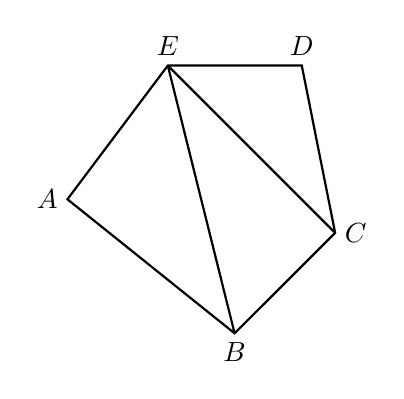
\begin{tikzpicture}
                \coordinate (A) at (0, 1.702125);
                \coordinate (B) at (2.122875, 0);
                \coordinate (C) at (3.4, 1.275);
                \coordinate (D) at (2.976125, 3.4);
                \coordinate (E) at (1.275, 3.4);

                \draw[thick] (A) -- (B) -- (C) -- (D) -- (E) -- cycle;
                \draw[thick] (B) -- (E);
                \draw[thick] (C) -- (E);

                \tikzhalflengtharrow{[xshift=-4.4625pt]B}{[xshift=-4.4625pt]E}
                \tikzhalflengtharrow{[xshift=4.4625pt]E}{[xshift=4.4625pt]B}
                \tikzhalflengtharrow{[yshift=-7.14pt]E}{[yshift=-7.14pt]A}
                \tikzhalflengtharrow{[yshift=7.14pt]B}{[yshift=7.14pt]C}
                \tikzhalflengtharrow{[yshift=6.05625pt]A}{[yshift=6.05625pt]B}
                \tikzhalflengtharrow{[yshift=-5.9925pt]C}{[yshift=-5.9925pt]E}
                \tikzhalflengtharrow{[xshift=5.9925pt]E}{[xshift=5.9925pt]C}
                \tikzhalflengtharrow{[yshift=-4.4625pt]D}{[yshift=-4.4625pt]E}
                \tikzhalflengtharrow{[xshift=-4.55175pt]C}{[xshift=-4.55175pt]D}

                \node[anchor=east] at (A) {\(A\)};
                \node[anchor=north] at (B) {\(B\)};
                \node[anchor=west] at (C) {\(C\)};
                \node[anchor=south] at (D) {\(D\)};
                \node[anchor=south] at (E) {\(E\)};
            \end{tikzpicture}
            \caption{Closed triangulated polygonal chain}\label{fig:cauchyintegraltheoremoversimplyconnectedset_closedpolygonalchaintriangulation}
        \end{minipage}
        \hfill
        \begin{minipage}{0.48\textwidth}
            \centering
            \vspace{0pt}
            \begin{tikzpicture}
                \coordinate (A) at (0, 0);
                \coordinate (D) at (4.14375, 1.59375);
                \coordinate (F) at (1.59375, 1.59375);
                \coordinate (C) at (5.1, 0);
                \coordinate (B) at (3.1875, 3.1875);
                \coordinate (E) at (2.55, 0);

                \draw[thick] (A) -- (F) -- (E) -- cycle;
                \draw[thick] (B) -- (D) -- (F) -- cycle;
                \draw[thick] (C) -- (D) -- (E) -- cycle;

                \tikzhalflengtharrow{[yshift=-7.45875pt]F}{[shift={(12.75pt,5.2275pt)}]A}
                \tikzhalflengtharrow{[yshift=-7.45875pt]B}{[shift={(12.75pt,5.2275pt)}]F}
                \tikzhalflengtharrow{[yshift=-7.45875pt]D}{[shift={(12.75pt,5.2275pt)}]E}
                \tikzhalflengtharrow{[yshift=7.45875pt]E}{[shift={(-12.75pt,-5.2275pt)}]D}

                \tikzhalflengtharrow{[shift={(-2.811375pt,-4.8705pt)}]E}{[shift={(-2.811375pt,-4.8705pt)}]F}
                \tikzhalflengtharrow{[shift={(-2.811375pt,-4.8705pt)}]D}{[shift={(-2.811375pt,-4.8705pt)}]B}
                \tikzhalflengtharrow{[shift={(-2.811375pt,-4.8705pt)}]C}{[shift={(-2.811375pt,-4.8705pt)}]D}
                \tikzhalflengtharrow{[shift={(2.811375pt,4.8705pt)}]F}{[shift={(2.811375pt,4.8705pt)}]E}

                \tikzhalflengtharrow{[yshift=4.8705pt]A}{[yshift=4.8705pt]E}
                \tikzhalflengtharrow{[yshift=4.8705pt]E}{[yshift=4.8705pt]C}
                \tikzhalflengtharrow{[yshift=4.8705pt]F}{[yshift=4.8705pt]D}
                \tikzhalflengtharrow{[yshift=-4.8705pt]D}{[yshift=-4.8705pt]F}

                \coordinate (AE) at ($(A)!0.5!(E)$);
                \coordinate (AF) at ($(A)!0.5!(F)$);
                \coordinate (FD) at ($(F)!0.5!(D)$);
                \coordinate (BF) at ($(B)!0.5!(F)$);
                \coordinate (EC) at ($(E)!0.5!(C)$);

                \path let
                \p1 = (FD),
                \p2 = (BF),
                \p3 = (AE),
                \p4 = (AF),
                \p5 = (EC)
                in
                node[shift={(3.1875pt,-3.1875pt)}] at (\x1, \y2) {\(\Delta_1\)}
                node[shift={(3.1875pt,-3.1875pt)}] at (\x3, \y4) {\(\Delta_2\)}
                node[shift={(3.1875pt,-3.1875pt)}] at (\x5, \y4) {\(\Delta_3\)}
                node[shift={(-3.1875pt, 3.1875pt)}] at (\x1, \y4) {\(\Delta_4\)};
            \end{tikzpicture}
            \caption{Quadrisection of \(\operatorname{int}\Delta\)}\label{fig:cauchyintegraltheoremoversimplyconnectedset_trianglequadrisection}
        \end{minipage}
    \end{figure}Since \(P\) is a closed polygonal chain, we can triangulate the interior. For example, consider \cref{fig:cauchyintegraltheoremoversimplyconnectedset_closedpolygonalchaintriangulation}. Then,
    \begin{align*}
        \int_{ABCDE}f(z)\ddz & =\qty(\int_{\overrightarrow{AB}}+\int_{\overrightarrow{BC}}+\int_{\overrightarrow{CD}}+\int_{\overrightarrow{DE}}+\int_{\overrightarrow{EA}})f(z)\ddz \\
        & \quad+\qty(\int_{\overrightarrow{BE}}+\int_{\overrightarrow{EB}}+\int_{\overrightarrow{CE}}+\int_{\overrightarrow{EC}})f(z)\ddz                       \\
        & =\int_{\Delta{ABE}}f(z)\ddz+\int_{\Delta{BCE}}f(z)\ddz+\int_{\Delta{CDE}}f(z)\ddz.
    \end{align*} Thus, if the integral over every triangle in \(U\) vanishes, then \cref{eq:cauchyintegraltheoremoversimplyconnectedset_statement} follows. Consider a triangle in \(U\) with boundary \(\Delta\). Then define \(M\) to be \[M=\abs{\int_{\Delta}f(z)\ddz}.\]
    We can quadrisect the triangle bounded by \(\Delta\) into four triangles with
    boundaries \(\Delta_1,\Delta_2,\Delta_3,\Delta_4\) as in
    \cref{fig:cauchyintegraltheoremoversimplyconnectedset_trianglequadrisection}.
    Then one of \(\Delta_1\), \(\Delta_2\), \(\Delta_3\), or \(\Delta_4\) (denote
    this to be \(\Delta^1\)) satisfy
    \[\abs{\int_{\Delta^1}f(z)\ddz}\geq\frac{M}{4},\]
    and recursively, choose
    \begin{equation}
        \abs{\int_{\Delta^2}f(z)\ddz}\geq\frac{M}{4^2},\ldots,\abs{\int_{\Delta^n}f(z)\ddz}\geq\frac{M}{4^n}. \label{eq:cauchyintegraltheoremoversimplyconnectedset_trianglelowerbound}
    \end{equation}
    Let \(L\) denote the perimeter of \(\Delta\). Then, the perimeters of \(\Delta^1,\Delta^2,\ldots\) respectively are \(\frac{L}{2},\frac{L}{2^2},\ldots\). As \(n\to\infty\), \(\Delta_n\) shrinks to a single point \(z_0\). Then, \(\forall n\in\mathbb{N}\), \(z_0\in\Delta^n\).

    By the definition of holomorphy, \(\forall\varepsilon>0\), \(\exists\delta>0\)
    such that \(\forall z\in D\paren{z_0,\delta}\), \[\abs{\frac{f\paren{z}-f\paren{z_0}}{z-z_0}-f'\paren{z_0}}<\varepsilon,\]\[\abs{f\paren{z}-f\paren{z_0}-f'\paren{z_0}\paren{z-z_0}}<\varepsilon\abs{z-z_0},\] and \(\exists N\in\mathbb{N}\) such that \(\forall n\in\mathbb{N}_{>N}\),
    \(\Delta^n\subset D\paren{z_0,\delta}\). By \cref{thm:cauchyintegraltheorem},
    since the functions \(z\mapsto 1\) and \(z\mapsto z\) are both entire, \[\int_{\Delta^n}\ddz=0,\quad\int_{\Delta^n}z\ddz=0.\] Then
    \begin{align*}
        \int_{\Delta^n}f(z)\ddz & =\int_{\Delta^n}f(z)\ddz-f\paren{z_0}\int_{\Delta^n}\ddz-f'\paren{z_0}\qty(\int_{\Delta^n}z\ddz-z_0\int_{\Delta^n}\ddz) \\
        & =\int_{\Delta^n}\brackets{f(z)-f\paren{z_0}-f'\paren{z_0}\paren{z-z_0}}\ddz.
    \end{align*}
    Because the distance between any two points in the interior of a triangle is always less than its perimeter, using the triangle inequality for complex integrals, \[\int_{\Delta^n}\abs{f(z)}\abs{\ddz}\leq\varepsilon\int_{\Delta^n}\abs{z-z_0}\abs{\ddz}=\frac{\varepsilon L}{2^n}\int_{\Delta^n}\abs{\ddz}=\frac{\varepsilon L^2}{4^n}.\]
    Comparing the above equation with
    \cref{eq:cauchyintegraltheoremoversimplyconnectedset_trianglelowerbound}, \[\frac{M}{4^n}<\frac{\varepsilon L}{4^n},\quad M<\varepsilon L.\] Since \(\Delta\) is rectifiable, \(L\) is finite, and letting
    \(\varepsilon\to0\), we find that \(M\to0\). Then, for every triangle in \(U\),
    the integral vanishes, and
    \cref{eq:cauchyintegraltheoremoversimplyconnectedset_chainvanishingstatement,eq:cauchyintegraltheoremoversimplyconnectedset_chaindefinition}
    follow.
\end{proof}
\begin{theorem}[\textsc{Cauchy--Goursat}]\label{thm:cauchygoursattheorem}
    Let \(U\subset\mathbb{C}\) be an open region bounded with boundary \(\partial U\). Let \(f:U\to\mathbb{C}\) be a holomorphic function continuous on \(\overline{U}\). Then, \[\oint_{\partial U}f(\zeta)\ddzeta=0.\]
\end{theorem}
\begin{proof}
    Since \(\partial U\cap U=\varnothing\) and \(f(z)\) is not necessarily holomorphic over \(\overline{U}\), we cannot directly apply \cref{lem:cauchyintegraltheoremoversimplyconnectedset}.
    \begin{figure}
        \centering
        \begin{tikzpicture}[>=stealth,
                arrow style/.style={
                    postaction={decorate},
                    decoration={markings, mark=at position 0.5 with {\arrow[scale=1]{Stealth}}}
            }]
            \pgfmathsetmacro{\lengtheta}{18pt}
            \pgfmathsetmacro{\lengthepsilon}{20pt}
            \coordinate (M) at (1, 1.5);
            \coordinate (P) at (1, 4.2);
            \coordinate (Q) at (5, 4.4);
            \coordinate (N) at (5, 1.7);
            \coordinate (Mprime) at ([yshift=\lengtheta] M);
            \coordinate (Pprime) at ([yshift=-\lengtheta] P);
            \coordinate (Qprime) at ([yshift=-\lengtheta] Q);
            \coordinate (Nprime) at ([yshift=\lengtheta] N);
            \draw[-{Stealth}, thick] (-0.5, 0) -- (6, 0);
            \draw[-{Stealth}, thick] (0, -0.5) -- (0, 6);
            \draw[thick, arrow style] (P) -- (M);
            \draw[thick, arrow style, name path=curveQP] (Q) to[out angle=90, in angle=90, curve through = {([shift={(2, 0)}] P) ([shift={(1.5, 0.2)}] P)}] (P);
            \draw[thick, arrow style] (N) -- (Q);
            \draw[thick, arrow style, name path=curveMN] (M) to[out angle=270, in angle=270, curve through = {([shift={(-2, 0)}] N) ([shift={(-1.5, -0.2)}] N)}] (N);
            \path let \p1 = (P) in coordinate (P1x) at ({\x1 + \lengthepsilon}, 0);
            \path let \p1 = (Q) in coordinate (Q1x) at ({\x1 - \lengthepsilon}, 0);
            \path[name path=verticalleftmarker](P1x) -- (P1x |- 0, 6);
            \path[name path=verticalrightmarker](Q1x) -- (Q1x |- 0, 6);
            \path[name intersections={of=curveQP and verticalleftmarker, by=P1}];
            \path[name intersections={of=curveMN and verticalleftmarker, by=M1}];
            \draw[thin] (M1) -- (P1);
            \path[name intersections={of=curveQP and verticalrightmarker, by=Q1}];
            \path[name intersections={of=curveMN and verticalrightmarker, by=N1}];
            \draw[thin] (N1) -- (Q1);
            \draw[thin] (Mprime) to[out angle=270, in angle=270, curve through = {([shift={(-2, 0)}] Nprime) ([shift={(-1.5, -0.2)}] Nprime)}] (Nprime);
            \draw[thin] (Qprime) to[out angle=90, in angle=90, curve through = {([shift={(2, 0)}] Pprime) ([shift={(1.5, 0.2)}] Pprime)}] (Pprime);
            \draw[dashed] (M) -- (M |- 0, 0);
            \draw[dashed] (N) -- (N |- 0, 0);
            \draw[dashed] (M1) -- (P1x);
            \draw[dashed] (N1) -- (Q1x);
            \node[anchor=north east] at (M) {\(M\)};
            \node[anchor=south east] at (P) {\(P\)};
            \node[anchor=south west] at (Q) {\(Q\)};
            \node[anchor=north west] at (N) {\(N\)};
            \node[anchor=north east] at (Mprime) {\(M'\)};
            \node[anchor=south east] at (Pprime) {\(P'\)};
            \node[anchor=south west] at (Qprime) {\(Q'\)};
            \node[anchor=north west] at (Nprime) {\(N'\)};
            \node[anchor=north west] at (M1) {\(M_1\)};
            \node[anchor=south] at (P1) {\(P_1\)};
            \node[anchor=south] at (Q1) {\(Q_1\)};
            \node[anchor=north east] at (N1) {\(N_1\)};
            \node[anchor=south west] at ([yshift=\lengtheta+7pt] M1) {\(M'_1\)};
            \node[anchor=north west] at ([yshift=-\lengtheta-3pt] P1) {\(P'_1\)};
            \node[anchor=north east] at ([yshift=-\lengtheta-7pt] Q1) {\(Q'_1\)};
            \node[anchor=south east] at ([yshift=\lengtheta+3pt] N1) {\(N'_1\)};
            \node[anchor=north] at (M |- 0, 0) {\(a\)};
            \node[anchor=north] at (N |- 0, 0) {\(b\)};
            \node[anchor=north] at (P1x |- 0, 0) {\(a+\varepsilon\)};
            \node[anchor=north] at (Q1x |- 0, 0) {\(b-\varepsilon\)};
            \node[anchor=north, xshift=-2pt] at (6, 0) {\(x\)};
            \node[anchor=east, yshift=-2pt] at (0, 6) {\(y\)};
        \end{tikzpicture}
        \caption{A simplified region containing two vertical lines and two continuous, rectifiable curves.}
        \label{fig:cauchygoursattheorem_simplifiedregion}
    \end{figure}

    First assume \(U\) has the shape of \(MNQP\) in
    \cref{fig:cauchygoursattheorem_simplifiedregion}. That is, \(U\) consists of
    \(x=a\), \(x=b\) for \(a<b\), and two rectifiable \(C^0\) curves
    \(\overrightarrow{MN}:y=\varphi(x)\) and \(\overrightarrow{QP}:\psi(x)\) such
    that \(\varphi(x)<\psi(x)\), \(\forall a\le x\le b\).

    For some \(\varepsilon>0\), \(\eta>0\), construct a new curve
    \(M_1'N_1'Q_1'P_1'\in U\) to be the boundary of the region bounded by
    \(P_1M_1:x=a+\varepsilon\), \(N_1Q_1:b-\varepsilon\), \(M'N':\varphi(x)+\eta\),
    and \(Q'P':\psi(x)-\eta\) such that \(M_1'N_1'Q_1'P_1'\) remains simple. By
    \cref{lem:cauchyintegraltheoremoversimplyconnectedset}, \[\oint_{M_1'N_1'Q_1'P_1'}f(z)\ddz=0.\]
    By \cref{thm:heinecantor}, \(f(z)\) is uniformly continuous over
    \(\overline{U}\), and therefore \(\forall\varepsilon'>0\), we can choose
    \(\eta>0\) so that \(\forall z\in\overrightarrow{M_1'N_1'}\),
    \(\abs{f\paren{z}-f\paren{z-\eta}}<\varepsilon'\) is satisfied. Letting
    \(\eta\to0\) (with \(\varepsilon'\to0\)) and fixing \(\varepsilon>0\), we get
    that
    \begin{align*}
        \abs{\int_{\overrightarrow{M_1'N_1'}}f(z)\ddz-\int_{\overrightarrow{M_1N_1}}f(z)\ddz} & \leq\int_{\overrightarrow{M_1'N_1'}}\abs{f(z)-f\paren{z-\eta}}\abs{\ddz} \\
        & <\varepsilon'\int_{\overrightarrow{M_1'N_1'}}\abs{dz}\to0,
    \end{align*}
    and consequently,
    \begin{equation}
        \int_{\overrightarrow{M_1'N_1'}}f(z)\ddz\to\int_{\overrightarrow{M_1N_1}}f(z)\ddz.\label{eq:cauchygoursattheorem_innerinnerhorizontaltoouterinnerhorizontal1}
    \end{equation}
    Under the same limit, we get
    \begin{equation}
        \int_{\overrightarrow{Q_1'P_1'}}f(z)\ddz\to\int_{\overrightarrow{Q_1P_1}}f(z)\ddz.\label{eq:cauchygoursattheorem_innerinnerhorizontaltoouterinnerhorizontal2}
    \end{equation} By the continuity of \(f(z)\) over a compact set,
    \begin{equation}
        \int_{\overrightarrow{P_1'M_1'}}f(z)\ddz\to\int_{\overrightarrow{P_1M_1}}f(z)\ddz,\quad\int_{\overrightarrow{N_1'Q_1'}}f(z)\ddz\to\int_{\overrightarrow{N_1Q_1}}f(z)\ddz.\label{eq:cauchygoursattheorem_innerinnerverticaltoouterinnervertical}
    \end{equation}
    Then letting \(\varepsilon\to0\), for the same reason as \cref{eq:cauchygoursattheorem_innerinnerverticaltoouterinnervertical}, \cref{eq:cauchygoursattheorem_innerinnerhorizontaltoouterinnerhorizontal1,eq:cauchygoursattheorem_innerinnerhorizontaltoouterinnerhorizontal2} yield \[\int_{\overrightarrow{M_1N_1}}f(z)\ddz\to\int_{\overrightarrow{MN}}f(z)\ddz,\quad\int_{\overrightarrow{Q_1P_1}}f(z)\ddz\to\int_{\overrightarrow{QP}}f(z)\ddz.\]
    We are left to show the subsequent limits of the results from
    \cref{eq:cauchygoursattheorem_innerinnerverticaltoouterinnervertical}. For the
    left integral, let
    \(y_{\varphi}=\max\cbraces{\varphi(a),\varphi\paren{a+\varepsilon}}\) and
    \(y_{\psi}=\max\cbraces{\psi(a),\psi\paren{a+\varepsilon}}\).

    Then, \[\int_{\overrightarrow{PM}}f(z)\ddz=\ii\int_{\psi(a)}^{\varphi(a)}f\paren{a+\ii y}\ddy=\ii\paren{\int_{\psi(a)}^{y_\varphi}+\int_{y_\varphi}^{y_\psi}+\int_{y_\psi}^{\varphi(a)}}f(a+\ii y)\ddy.\]
    Similarly, \[\int_{\overrightarrow{P_1M_1}}f(z)\ddz=\ii\paren{\int_{\psi(a+\varepsilon)}^{y_\varphi}+\int_{y_\varphi}^{y_\psi}+\int_{y_\psi}^{\varphi(a+\varepsilon)}}f(a+\varepsilon+\ii y)\ddy.\]
    The difference
    \(\paren{\int_{\overrightarrow{PM}}-\int_{\overrightarrow{P_1M_1}}}f(z)\ddz\)
    between the two is then equal to
    \begin{gather*}
        \ii\int_{y_{\varphi}}^{y_{\psi}}\paren{f\paren{a+\ii y}-f\paren{a+\varepsilon+\ii y}}\ddz\\
        {}+{\ii\paren{\int_{\psi(a)}^{y_\varphi}+\int_{y_\psi}^{\varphi(a)}}f(a+\ii y)-\ii\paren{\int_{\psi(a+\varepsilon)}^{y_\varphi}z+\int_{y_\psi}^{\varphi\paren{a+\varepsilon}}}f(a+\varepsilon+\ii y)}.
    \end{gather*}
    The first term vanishes by uniform continuity (through the same argument used for \(M_1'N_1'\to M_1N_1\)) and the remaining four integrals all equal 0 as they are all integrable on a degenerating interval (as \(\varepsilon\to0\), \(y_\varphi\to\varphi(a)\) and \(y_\psi\to\psi(a)\) because \(\varphi,\psi\in C^0\)). Therefore, \[\int_{\overrightarrow{P_1M_1}}f(z)\ddz\to\int_{\overrightarrow{PM}}f(z)\ddz,\]
    and through similar logic, \[\int_{\overrightarrow{N_1Q_1}}f(z)\ddz\to\int_{\overrightarrow{NQ}}f(z)\ddz.\] Therefore, \[\oint_{MNQP}f(z)\ddz=0.\]
    Any open region \(U\subset\mathbb{C}\) with a simple closed boundary can be
    broken up into smaller regions with the same form as \(MNQP\) with finitely
    many auxiliary lines. Then the conclusion follows.
\end{proof}
\begin{remark}
    The theorem is also valid for any multiply connected region (and its boundary will consist of multiple curves) as a multiply connected region is equal to the union of several simply connected regions with vertical auxiliary lines between.

    Additionally, if \(U\subset\mathbb{C}\) is simply connected and \(f\) is
    holomorphic on \(U\), then for any two points \(z,z_0\in U\), the integral \[\int_{z_0}^z f(\zeta)\ddzeta\] is well-defined and independent of the path taken from \(z_0\) to \(z\). In
    this sense, a holomorphic function behaves analogously to a potential field.
\end{remark}
\begin{theorem}[\textsc{Cauchy--Goursat}]\label{thm:cauchygoursatformula}
    Let \(U\subset\mathbb{C}\) be an open region bounded with a simple closed boundary \(\partial U\), and let \(f:U\to\mathbb{C}\) be a holomorphic function continuous on \(\overline{U}\). Then for all \(z\in U\),
    \begin{equation}
        f(z)=\frac{1}{2\piup\ii}\oint_{\partial U}\frac{f(\zeta)}{\zeta-z}\ddzeta.\label{eq:cauchygoursatformula}
    \end{equation}
\end{theorem}
\begin{proof}
    By the Cauchy--Goursat Theorem (\cref{thm:cauchygoursattheorem}), \[\int_{\partial\paren{U\setminus D(z,\varepsilon)}}\frac{f(\zeta)}{\zeta-z}\ddzeta=\oint_{\partial U}\frac{f(\zeta)}{\zeta-z}\ddzeta-\oint_{\partial D(z,\varepsilon)}\frac{f(\zeta)}{\zeta-z}\ddzeta=0.\]
    From rearrangement, \[\oint_{\partial U}\frac{f(\zeta)}{\zeta-z}\ddzeta=2\piup\ii f(z)+\ii\int_0^{2\piup}\paren{f\paren{z+\varepsilon\ee^{\ii t}}-f(z)}\dd{t}.\]
    Since \(f\in C^0(\partial D(z,\varepsilon))\), as \(\varepsilon\to0\),
    \begin{align*}
        \abs{\int_0^{2\piup}\paren{f\paren{z+\varepsilon\ee^{\ii t}}-f(z)}\dd{t}} & \leq\int_0^{2\piup}\abs{f\paren{z+\varepsilon\ee^{\ii t}}-f(z)}\dd{t}            \\
        & \leq2\piup\max_{t\in[0,2\piup]}\abs{f\paren{z+\varepsilon\ee^{\ii t}}-f(z)}\to0.
    \end{align*}
    By rearrangement, \[f(z)=\frac{1}{2\piup\ii}\oint_{\partial U}\frac{f(\zeta)}{\zeta-z}\ddzeta.\qedhere\]
\end{proof}
\begin{remark}
    In the proof of \cref{thm:pompeiu}, we used Lipschitz continuity for a smooth function, which was a stronger condition than necessary. The true necessity of smoothness was to be able to apply Green's Theorem (\cref{thm:complexgreen}).
\end{remark}
This profound theorem is extremely important and helpful in complex integration and essential in the evaluation of integrals, as demonstrated below.
\begin{example}\label{ex:cauchygoursatformulazeroofunity}
    Evaluate the integral \(\oint_{\partial D(0,2)}\frac{\ddz}{z^n-1}\), where \(n\in\mathbb{N}_{\geq 2}\).
\end{example}
\begin{proof}
    Since \(z^n-1=\prod_{k=0}^{n-1}\qty(z-\omega^k_n)\), where \(\omega^k_n=\ee^{\ii\piup\frac{k}{n}}\), the integrand has singularities at every \(n\)-th zero of unity. Then the integral is equal to:
    \begin{equation}
        \oint_{\partial D(0,2)}\frac{\ddz}{\prod_{j=0}^{n-1}\qty(z-\omega_j)}=\oint_{\partial D(0,2)}\sum_{j=0}^{n-1}\frac{c_j}{z-\omega_j}\ddz,\label{eq:cauchygoursatformulazerosofunity}
    \end{equation}
    where \(\cbraces{c_j}\) are the coefficients of the partial fraction decomposition. By the Cauchy--Goursat Formula (\cref{thm:cauchygoursatformula}), \cref{eq:cauchygoursatformulazerosofunity} becomes: \[\sum_{k=0}^{n-1}\oint_{\partial D(0,2)}\frac{c_k}{z-\omega_k}\ddz=2\piup\ii\sum_{k=0}^{n-1}c_k.\]
    Observe that \(\sum_{k=0}^{n-1}
    c_k=\lim_{z\to\infty}\sum_{k=0}^{n-1}\frac{zc_k}{z-\omega_k}=\lim_{z\to\infty}\frac{z}{z^n-1}=0\)
    since \(n\geq2\). Therefore, \[\oint_{\partial D(0,2)}\frac{\ddz}{z^n-1}=0.\qedhere\]
\end{proof}
We have also already seen the utility of parameterization via a polar transformation. Many useful identities in classical calculus can also be derived from concepts in its generalization:
\begin{example}
    Prove that \(\forall n\in\mathbb{N}\), \[\int_{0}^{2\piup}\cos^{2n}\theta\dd{\theta}=2\piup\prod_{k=1}^n\frac{2k-1}{2k}.\]
\end{example}
\begin{proof}
    Consider the integral \[\oint_{\partial\mathbb{D}}\qty(z+\frac{1}{z})^{2n}\frac{\ddz}{z}.\]
    Letting \(z=\ee^{\ii\theta}\), we get
    \(\oint_{\partial\mathbb{D}}\qty(\ee^{\ii\theta}+\ee^{-\ii\theta})^{2n}\ee^{-\ii\theta}\ddz=2^{2n}\ii\int_0^{2\piup}\cos^{2n}\theta\dd{\theta}\).
    Alternatively, we can expand the integrand and get \[\oint_{\partial\mathbb{D}}\sum_{k=0}^{2n}\binom{2n}{k}z^{2k-2n}\frac{\ddz}{z}=\sum_{k=0}^{2n}\oint_{\partial\mathbb{D}}\binom{2n}{k}z^{2k-2n-1}\ddz.\]
    When \(2k-2n-1\ge0\), the integrand is holomorphic. The integral is then equal
    to \[\binom{2n}{0}\oint_{\partial\mathbb{D}}z^{-2n-1}\ddz+\binom{2n}{1}\oint_{\partial\mathbb{D}}z^{-2n+1}\ddz+\cdots+\binom{2n}{n}\oint_{\partial\mathbb{D}}\frac{\ddz}{z}=2\piup\ii\binom{2n}{n},\]
    since all the higher order terms vanish:
    \[\oint_{\partial\mathbb{D}}z^{2k-2n-1}\ddz=\ii\int_0^{2\piup}\ee^{2\ii\theta(k-n)}\dd{\theta}=
        \begin{dcases}
            0         & \qif* k<n, \\
            2\piup\ii & \qif* k=n.
    \end{dcases}\]
    Therefore, \[2^{2n}\ii\int_0^{2\piup}\cos^{2n}\theta\dd{\theta}=2\piup\ii\binom{2n}{n}\Longleftrightarrow\int_0^{2\piup}\cos^{2n}\theta\dd{\theta}=\frac{2\piup\qty(2n)!}{2^{2n}\qty(n!)^2}=\frac{2\piup\prod_{k=1}^{2n}k}{\prod_{k=1}^{n}{\qty(2k)}^2}.\]
    From simple cancellation, we get \[2\piup\frac{\prod_{k=1}^{n}\qty(2k-1)}{\prod_{k=1}^n\qty(2k)}=2\piup\prod_{k=1}^n\frac{2k-1}{2k},\]
    as expected.
\end{proof}
\begin{example}[Cauchy--Goursat Formula on the Exterior]\label{ex:cauchygoursatformulaexterior}
    Let \(\gamma\subset\mathbb{C}\) be a simple closed curve, and suppose that \(f:\mathrm{ext}(\gamma)\to\mathbb{C}\) is holomorphic and continuous on \(\overline{\mathrm{ext}(\gamma)}=\mathbb{C}\setminus\mathrm{int}(\gamma)\), where \(\mathrm{int}\) and \(\mathrm{ext}\) respectively denote the interior and exterior as in \cref{thm:jordancurve}.
    \begin{enumerate}
        \item If \(f\) has a removable singularity at \(\infty\), or if \(w=\lim_{z\to\infty}
            f(z)\) exists and is finite, then \(\forall z\in\mathbb{C}\setminus\gamma\), \[\frac{1}{2\piup\ii}\oint_\gamma\frac{f(\zeta)}{\zeta-z}\ddzeta=
                \begin{dcases}
                    w      & \qif* z\in\mathrm{int}(\gamma), \\
                    w-f(z) & \qif* z\in\mathrm{ext}(\gamma).
            \end{dcases}\]
        \item If \(\gamma\) encloses the origin, then \(\forall
            z\in\mathbb{C}\setminus\gamma\), then
            \begin{equation}
                \frac{1}{2\piup\ii}\oint_\gamma\frac{zf(\zeta)}{z\zeta-\zeta^2}\ddzeta=
                \begin{dcases}
                    0    & \qif* z\in\mathrm{int}(\gamma),                                                       \\
                    f(z) & \qif* z\in\mathrm{ext}(\gamma).\label{eq:cauchygoursatformulaexteriorpart2_statement}
                \end{dcases}
            \end{equation}
    \end{enumerate}
\end{example}
\begin{proof}
    \begin{enumerate}
        \item By the compactness of \(\gamma\), it can be completely contained within a
            sufficiently large disk centered at the origin (\(\gamma\subset D(0,R)\)). Then
            by applying \cref{thm:cauchygoursatformula} or \cref{thm:cauchygoursattheorem}
            on the set
            \(D(0,R)\cap\mathrm{ext}(\gamma)=D(0,R)\setminus\overline{\mathrm{int}(\gamma)}\),
            we get that \[\frac{1}{2\piup\ii}\oint_{\partial D(0,R)}\frac{f(\zeta)}{\zeta-z}\ddzeta=\frac{1}{2\piup\ii}\oint_\gamma\frac{f(\zeta)}{\zeta-z}\ddzeta+
                \begin{dcases}
                    0    & \qif* z\in\mathrm{int}(\gamma),            \\
                    f(z) & \qif* z\in D(0,R)\cap\mathrm{ext}(\gamma).
            \end{dcases}\]
            By letting \(R\to\infty\) and letting \(\zeta=R\ee^{\ii\theta}\), we get that \[\frac{1}{2\piup\ii}\oint_\gamma\frac{f(\zeta)}{\zeta-z}\ddzeta=\frac{1}{2\piup}\lim_{R\to\infty}\int_0^{2\piup}\frac{f\qty(R\ee^{\ii\theta})}{1-\frac{z}{R\ee^{\ii\theta}}}\dd{\theta}-
                \begin{dcases}
                    0    & \qif* z\in\mathrm{int}(\gamma), \\
                    f(z) & \qif* z\in\mathrm{ext}(\gamma).
            \end{dcases}\]
            By the continuity of \(f\) on \(\partial D(0,R)\), it attains its maximum
            \(M\). For sufficiently large \(R\), \(\abs{1-\frac{z}{R\ee^{\ii\theta}}}\)
            attains a positive minimum. Then the integrand is uniformly bounded in \(R\)
            and \(\theta\), and hence the order of the limit and the integral may be
            exchanged. Hence,
            \begin{align*}
                \frac{1}{2\piup\ii}\oint_\gamma\frac{f(\zeta)}{\zeta-z}\ddzeta & =\frac{1}{2\piup}\int_0^{2\piup}\frac{w}{1-\lim_{R\to\infty}\frac{z}{R\ee^{\ii\theta}}}\dd{\theta}-
                \begin{dcases}
                    0    & \qif* z\in\mathrm{int}(\gamma), \\
                    f(z) & \qif* z\in\mathrm{ext}(\gamma),
                \end{dcases}                                                                                                                               \\       & =
                \begin{dcases}
                    w      & \qif* z\in\mathrm{int}(\gamma), \\
                    w-f(z) & \qif* z\in\mathrm{ext}(\gamma),
                \end{dcases}
            \end{align*} as expected.
        \item Under the partial fraction decomposition of
            \cref{eq:cauchygoursatformulaexteriorpart2_statement}, we get that
            \begin{align}
                I & =\oint_\gamma\frac{zf(\zeta)}{z\zeta-\zeta^2}\ddzeta=\oint_\gamma\qty(\frac{f(\zeta)}{\zeta}-\frac{f(\zeta)}{\zeta-z})\ddzeta\nonumber \\
                & =\int_0^{2\piup}\qty(f\qty(R\ee^{\ii\theta})-\frac{f\qty(R\ee^{\ii\theta})}{1-\frac{z}{R\ee^{\ii\theta}}})\dd{\theta}+
                \begin{dcases}
                    0              & \qif* z\in\mathrm{int}(\gamma),            \\
                    2\piup\ii f(z) & \qif* z\in\mathrm{ext}(\gamma)\cap D(0,R),
                \end{dcases}\label{eq:cauchygoursatformulaexteriorpart2_prelimitintegral}
            \end{align} when \(\gamma\subset D(0,R)\).
            We will analyze the first integral as \(R\to\infty\). By the triangle and reverse triangle inequalities,
            \begin{align*}
                \qty|\int_0^{2\piup}\qty(f\qty(R\ee^{\ii\theta})-\frac{f\qty(R\ee^{\ii\theta})}{1-\frac{z}{R\ee^{\ii\theta}}})\dd{\theta}| & \leq\int_0^{2\piup}\qty|\frac{z}{R\ee^{\ii\theta}-z}|\dd{\theta}                             \\
                & \leq\int_0^{2\piup}\frac{\abs{z}}{R-\abs{z}}\dd{\theta}=\frac{2\piup\abs{z}}{R-\abs{z}}\to0.
            \end{align*}
    \end{enumerate}
    By substituting the result into \cref{eq:cauchygoursatformulaexteriorpart2_prelimitintegral}, and letting \(R\to\infty\), we get that \[\frac{1}{2\piup\ii}\oint_\gamma\frac{zf(\zeta)}{z\zeta-\zeta^2}\ddzeta=
        \begin{dcases}
            0    & \qif* z\in\mathrm{int}(\gamma), \\
            f(z) & \qif* z\in\mathrm{ext}(\gamma),
    \end{dcases}\] as desired.
\end{proof}
\subsection{Analyticity and Holomorphy}\label{sec:analyticityandholomorphy}
The Cauchy--Goursat Formula (\cref{thm:cauchygoursatformula}) can also be
generalized into a result that equates complex integration and differentiation:
\begin{theorem}[\textsc{Cauchy--Goursat}]\label{thm:cauchydifferentiationformula}
    Let \(U\subset\mathbb{C}\) be an open region bounded by a simple closed boundary \(\partial U\), and let \(f:U\to\mathbb{C}\) be holomorphic and continuous over \(\overline{U}\). Then \(\forall z\in U\), \(\forall n\in\mathbb{N}\), \(f^{(n)}(z)\) exists, and
    \begin{equation}
        f^{(n)}(z)=\frac{n!}{2\piup\ii}\oint_{\partial U}\frac{f(\zeta)}{\paren{\zeta-z}^{n+1}}\ddzeta.\label{eq:cauchydifferentiationformula_statement}
    \end{equation}
    Additionally, since \(U\) is open, \(\forall z_0\in U\), \(\forall r>0\) such that the closed disk \(\overline{D\paren{z_0,r}}\subset U\), \(f\) has the uniformly and absolutely convergent Taylor expansion
    \begin{equation}
        f(z)=\sum_{j=0}^\infty a_j\paren{z-z_0}^j,\label{eq:cauchydifferentiationformula_taylorseries}
    \end{equation}
    where
    \begin{equation}
        a_j=\frac{1}{2\piup\ii}\oint_{\partial U}\frac{f(\zeta)}{\paren{\zeta-z}^{j+1}}\ddzeta\label{eq:cauchydifferentiationformula_taylorseriescoefficients}
    \end{equation} on \(\overline{D\paren{z_0,r}}\).
\end{theorem}
\begin{proof}
    \(\forall z_0\in U\), \(\forall z\in D\paren{z_0,r}\subset U\), by \cref{thm:cauchygoursatformula}, \[f(z)-f\paren{z_0}=\frac{1}{2\piup\ii}\oint_{\partial U}\paren{\frac{f(\zeta)}{\zeta-z}-\frac{f(\zeta)}{\zeta-z_0}}\ddzeta=\frac{z-z_0}{2\piup\ii}\oint_{\partial U}\frac{f(\zeta)\ddzeta}{\paren{\zeta-z}\paren{\zeta-z_0}},\]
    and dividing by \(z-z_0\), the above is equal to \[\frac{f(z)-f\paren{z_0}}{z-z_0}=\frac{1}{2\piup\ii}\oint_{\partial U}\frac{f(\zeta)\ddzeta}{\paren{\zeta-z}\paren{\zeta-z_0}}.\]
    Since
    \begin{align}
        \frac{f(z)-f\paren{z_0}}{z-z_0}-\frac{1}{2\piup\ii}\oint_{\partial U}\frac{f(\zeta)\ddzeta}{\paren{\zeta-z_0}^2} & =\frac{1}{2\piup\ii}\oint_{\partial U}\frac{f\paren{\zeta}}{\zeta-z_0}\paren{\frac{1}{\zeta-z}-\frac{1}{\zeta-z_0}}\ddzeta\nonumber                                      \\
        & =\frac{z-z_0}{2\piup\ii}\oint_{\partial U}\frac{f(\zeta)}{(\zeta-z)\paren{\zeta-z_0}^2}\ddzeta.\label{eq:cauchydifferentiationformula_differenceoffirstorderdifferences}
    \end{align}
    Let \(d\) be the distance from \(z_0\) to \(\partial U\), and it follows that \(0<r<d\). Then, since \(\abs{z-z_0}<r\) and \(\abs{\zeta-z_0}\geq d\), \(\abs{\zeta-z}\geq d-r\). Then the absolute value of the integrand of \cref{eq:cauchydifferentiationformula_differenceoffirstorderdifferences} is bounded above by \(\frac{M}{d^2(d-r)}\), where \(M\) is the maximum of \(f(\zeta)\), which exists by \cref{thm:continuousfunctionboundedoncompact}. Then, \[\abs{\frac{z-z_0}{2\piup\ii}\oint_{\partial U}\frac{f(\zeta)}{(\zeta-z)\paren{\zeta-z_0}^2}\ddzeta}\leq\frac{\abs{z-z_0}}{2\piup}\frac{M}{d^2(d-r)}\oint_{\partial U}\abs{\ddzeta}.\] As \(z\to z_0\), the difference vanishes, and therefore, \[f'\paren{z_0}=\frac{1}{2\piup\ii}\oint_{\partial U}\frac{f(\zeta)}{\paren{\zeta-z_0}^2}\ddzeta.\]
    Now inductively assume that \cref{eq:cauchydifferentiationformula_statement} is
    true for a given \(n=k\in\mathbb{N}\), or \[f^{(k)}(z)=\frac{k!}{2\piup\ii}\oint_{\partial U}\frac{f(\zeta)}{\paren{\zeta-z}^{k+1}}\ddzeta.\]
    Notice the expansion of the kernel, convergent since
    \(\abs{z-z_0}<\abs{\zeta-z_0}\):
    \begin{equation}
        \frac{1}{\zeta-z}=\frac{1}{\zeta-z_0}\cdot\frac{\zeta-z_0}{\zeta-z}=\frac{1}{\zeta-z_0}\cdot\frac{1}{1-\frac{z-z_0}{\zeta-z_0}}=\frac{1}{\zeta-z_0}\sum_{j=0}^{\infty}\paren{\frac{z-z_0}{\zeta-z_0}}^j.\label{eq:cauchydifferentiationformula_kernelexpansion}
    \end{equation}
    Then,
    \begin{align*}
        f^{(k)}(z) & =\frac{k!}{2\piup\ii}\oint_{\partial U}\frac{f(\zeta)}{(\zeta-z)^{k+1}}\ddzeta                                                                           \\
        & =\frac{k!}{2\piup\ii}\oint_{\partial U}\frac{f(\zeta)}{\paren{\zeta-z_0}^{k+1}}\paren{\sum_{j=0}^{\infty}\paren{\frac{z-z_0}{\zeta-z_0}}^j}^{k+1}\ddzeta \\
        & =f^{(k)}\paren{z_0}+\frac{(k+1)!\paren{z-z_0}}{2\piup\ii}\oint_{\partial U}\frac{f(\zeta)}{\paren{\zeta-z_0}^{k+2}}\ddzeta                               \\
        & \quad+\order{\abs{z-z_0}^2},
    \end{align*}
    where the remainder terms \(\order{\abs{z-z_0}^2}\) resemble
    \[\paren{z-z_0}^2\frac{k!}{2\piup\ii}\brackets{k+1+\binom{k+1}{2}}\oint_{\partial U}\frac{f(\zeta)}{\paren{\zeta-z_0}^{k+3}}\ddzeta+\order{\abs{z-z_0}^3}.\]
    The difference quotient is equal to \[\frac{f^{(k)}(z)-f^{(k)}\paren{z_0}}{z-z_0}=\frac{(k+1)!}{2\piup\ii}\oint_{\partial U}\frac{f(\zeta)}{\paren{\zeta-z_0}^{k+2}}\ddzeta+\order{\abs{z-z_0}}.\] As \(z\to z_0\), the remainder terms vanish, and \[f^{(k+1)}\paren{z_0}=\frac{(k+1)!}{2\piup\ii}\oint_{\partial U}\frac{f(\zeta)}{\paren{\zeta-z_0}^{k+2}}\ddzeta.\]
    By induction, \cref{eq:cauchydifferentiationformula_statement} is valid. By
    substituting \cref{eq:cauchydifferentiationformula_kernelexpansion} into
    \cref{eq:cauchygoursatformula}, we obtain \[f(z)=\frac{1}{2\piup\ii}\oint_{\partial U}\frac{f(\zeta)}{\zeta-z_0}\sum_{j=0}^{\infty}\paren{\frac{z-z_0}{\zeta-z_0}}^j\ddzeta=\frac{1}{2\piup\ii}\oint_{\partial U}\sum_{j=0}^{\infty}\paren{z-z_0}^j\frac{f(\zeta)\ddzeta}{\paren{\zeta-z_0}^{j+1}}.\]
    Because \(f(\zeta)\) is continuous over \(\partial U\), it is bounded by a
    constant \(M\). Additionally, since \(\abs{z-z_0}<\abs{\zeta-z_0}\), the sum is
    termwise bounded by the convergent series \[\sum_{j=0}^\infty\frac{Mr^j}{\inf_{\xi\in\partial U}\abs{\xi-z_0}^{j+1}}.\]
    By the Weierstrass \(M\)--Test (\cref{thm:weierstrassmtest}), the series
    uniformly converges, and we can justify
    \begin{gather*}
        \frac{1}{2\piup\ii}\oint_{\partial U}\sum_{j=0}^{\infty}\paren{z-z_0}^j\frac{f(\zeta)}{\paren{\zeta-z_0}^{j+1}}\ddzeta=\frac{1}{2\piup\ii}\sum_{j=0}^{\infty}\oint_{\partial U}\paren{z-z_0}^j\frac{f(\zeta)}{\paren{\zeta-z_0}^{j+1}}\ddzeta\\=\sum_{j=0}^\infty a_j\paren{z-z_0}^j,
    \end{gather*}
    which verifies \cref{eq:cauchydifferentiationformula_taylorseries,eq:cauchydifferentiationformula_taylorseriescoefficients}.
\end{proof}
\begin{remark}
    By induction, we have shown that assuming the existence of the first order derivative of a holomorphic function \(f\), the \(n\)-th order derivative of \(f\) exists \(\forall n\in\mathbb{N}\) and is holomorphic over the same region as \(f^{(n-1)}\). Furthermore, if \(f\) is holomorphic, then \(\forall z\in U\), there exists an open disk enclosing \(z\) such that \(f\) has a convergent Taylor series expansion. This property is known as \textscsl{analyticity}, and \cref{thm:cauchydifferentiationformula} tells us that all holomorphic functions are analytic. Analytic functions can be expanded into power series, which are termwise differentiable, and therefore complex differentiable. Thus, analyticity and holomorphy are logically equivalent, which is a fundamental difference between real and complex functions.
\end{remark}
The differentiation formula above can be thought of as a generalization of \cref{thm:cauchygoursatformula}, and provides similar utility in the evaluation of integrals:
\begin{example}\label{ex:legendrepolynomialintegralformula}
    A \textscsl{Legendre polynomial} is a polynomial whose explicit equation is given by
    \begin{equation}
        P_n(z)=\frac{1}{2^n n!}\dv[n]{z}({\qty(z^2-1)}^n).\label{eq:legendrepolynomialintegralformula_rodriguesformula}
    \end{equation}
    Prove the integral form \[P_n(z)=\frac{1}{2\piup\ii}\oint_\gamma\frac{{\qty(\zeta^2-1)}^n}{2^n{(\zeta-z)}^{n+1}}\ddzeta,\] where \(\gamma\) is a simple closed curve enclosing \(z\).
\end{example}
\begin{proof}
    By applying Cauchy--Goursat (\cref{thm:cauchydifferentiationformula}) on \cref{eq:legendrepolynomialintegralformula_rodriguesformula}, we get that \[P_n(z)=\frac{1}{2^{n+1}\piup\ii}\oint_{\gamma}\frac{{\qty(\zeta^2-1)}^n}{{(\zeta-z)}^{n+1}}\ddzeta,\] as desired.
\end{proof}
\begin{theorem}[\textsc{Cauchy's Estimate}]\label{thm:cauchysestimate}
    For a function \(f:U\to\mathbb{C}\) holomorphic over \(U\subseteq\mathbb{C}\) and \(\forall z_0\in U\) and \(\forall R>0\) such that \(\overline{D\paren{z_0,R}}\subseteq{U}\), \(\forall n\in\mathbb{N}\), \[\abs{f^{(n)}\paren{z_0}}\leq\frac{n!M}{R^n},\]
    where \[M=\max_{z\in\overline{D\paren{z_0,R}}}\abs{f(z)}.\]
\end{theorem}
\begin{proof}
    By the Differentiation Formula (\cref{thm:cauchydifferentiationformula}), \(\forall n\in\mathbb{N}\), \[f^{(n)}\paren{z_0}=\frac{n!}{2\piup\ii}\oint_{\partial D\paren{z_0,R}}\frac{f(\zeta)}{\paren{\zeta-z_0}^{n+1}}\ddzeta.\]
    Because \(f(z)\) is continuous over the boundary \(\partial D\paren{z_0,R}\),
    it is bounded by \(M\). Thus,
    \[\abs{f^{(n)}\paren{z_0}}\leq\frac{n!}{2\piup}\int_0^{2\piup}\frac{M}{\paren{\ee^{\ii\theta}R}^{n+1}}\ee^{\ii\theta}R\dd{\theta}=\frac{n!M}{R^n},\] as desired.
\end{proof}
\cref{thm:nthderivativeboundedl1norm} will profoundly generalize this statement significantly. The relationship between the derivatives of a holomorphic function and the function itself is an important property of holomorphic functions.
\begin{example}
    Let \(f\) be entire and \(\forall z\in\mathbb{C}\), \(\abs{f(z)}\leq M\ee^{\abs{z}}\). Prove that \(\forall n\in\mathbb{N}\), \(\abs{f(0)}\leq M\) and \[\abs{f^{(n)}(0)}\leq Mn!\qty(\frac{\ee}{n})^n.\]
\end{example}
\begin{proof}
    \(|f(0)|\leq M\) is obviously true by letting \(z=0\). Then \(\forall R>0\), by Cauchy's Estimate (\cref{thm:cauchysestimate}), \[\abs{f^{(n)}(0)}\leq Mn!\frac{\ee^{R}}{R^n}.\]
    By letting \(R=n\), the conclusion follows. In fact, this is the tightest
    possible inequality. Consider \(\varphi(R)=Mn!\frac{\ee^R}{R^n}\) to be a
    function of \(R\). It attains its minimum as its derivative vanishes:
    \[\varphi'(R)=Mn!\frac{\ee^RR^n-n\ee^RR^{n-1}}{R^{2n}}=0\Longleftrightarrow R^n=nR^{n-1}\Longleftrightarrow R=n.\] To confirm it as a minimum, we calculate the second order derivative:
    \[\varphi''(R)=Mn!\ee^R\qty(\frac{1}{R^n}-\frac{2n}{R^{n+1}}+\frac{n(n+1)}{R^{n+2}})\implies\varphi''(n)=M(n-1)!\frac{\ee^n}{n^n},\]
    which is positive and convex.
\end{proof}
The following theorem, albeit originally proven by Cauchy in 1844, shows a fundamental difference between holomorphic functions on proper subsets of \(\mathbb{C}\) and entire functions.
\begin{theorem}[\textsc{Liouville}]\label{thm:liouville}
    Any bounded entire function is constant.
\end{theorem}
\begin{proof}
    Let \(f:\mathbb{C}\to\mathbb{C}\) be entire. Then, \(\forall z_0\in\mathbb{C}\), \(\forall R>0\), \(f\) is holomorphic over \(\overline{D\paren{z_0,R}}\). By \cref{thm:cauchysestimate}, \[\abs{f'\paren{z_0}}\leq\frac{M}{R},\] where \(M=\sup_{z\in\mathbb{C}}\abs{f(z)}\). By letting \(R\to\infty\),
    \(f'\paren{z_0}\) where \(z_0\) is any arbitrary value in \(\mathbb{C}\).
    Therefore, \(f(z)\) is constant.
\end{proof}
\begin{proof}[Alternative Proof]
    Let \(a,b\in\mathbb{C}\) be distinct and arbitrarily chosen. Let
    \(f:\mathbb{C}\to\mathbb{C}\) be entire and bounded such that \(\abs{f}\leq M\)
    for some \(M>0\). Let \(R>\abs{a},\abs{b}\). Since \(a\neq b\),
    \(\exists\varepsilon>0\) such that
    \(\overline{D(a,\varepsilon)}\cup\overline{D(b,\varepsilon)}=\varnothing\). By
    the Cauchy--Goursat Theorem (\cref{thm:cauchygoursattheorem}), we have \[\oint_{\partial D(0,R)}\frac{f(z)}{(z-a)(z-b)}\ddz=\qty(\oint_{\partial D(a,\varepsilon)}+\oint_{\partial D(b,\varepsilon)})\frac{f(z)}{(z-a)(z-b)}\ddz.\]
    Since \(z\mapsto\frac{f(z)}{z-a}\) is holomorphic on the disk centered at \(b\)
    and \(z\mapsto\frac{f(z)}{z-b}\) is holomorphic on the disk centered at \(a\),
    by the Cauchy--Goursat Formula (\cref{thm:cauchygoursatformula}), we have \[\oint_{\partial D(0,R)}\frac{f(z)}{(z-a)(z-b)}\ddz=2\piup\ii\qty(\frac{f(b)}{b-a}+\frac{f(a)}{a-b}).\]
    On the contrary, we also have
    \begin{align*}
        \abs{\qty(\oint_{\partial D(a,\varepsilon)}+\oint_{\partial D(b,\varepsilon)})\frac{f(z)}{(z-a)(z-b)}\ddz} & \leq M\oint_{\partial D(0,R)}\frac{\abs{\ddz}}{\abs{z-a}\abs{z-b}} \\
        & =\frac{2\piup MR}{(R-a)(R-b)}                                      \\
        & \to 0\qas{R\to\infty}.
    \end{align*}
    We conclude that \[\frac{2\piup\ii}{b-a}\qty(f(b)-f(a))=0\] for all distinct complex \(a\) and \(b\). Hence, \(f\) is a constant function.
\end{proof}
\begin{theorem}[\textsc{Morera}]\label{thm:morera}
    Let \(U\subseteq\mathbb{C}\) and \(f:U\to\mathbb{C}\) be continuous over \(U\). If for any closed triangular contour \(\gamma\subset U\), \[\oint_{\gamma}f(\zeta)\ddzeta=0,\] then \(f\) is holomorphic over \(U\).
\end{theorem}
\begin{proof}
    Let \(z_0\in U\) be arbitrary. Since \(U\) is open, \(\exists r>0\) such that
    \(\overline{D}=\overline{D\qty(z_0,r)}\subset U\). Define \[F(z)=\int_{z_0}^z f(\zeta)\ddzeta,\] where the path is a straight line segment, and \(F\) is well-defined for \(z\in D\). Now \[F'(z)=\lim_{\Delta z\to 0}\frac{F(z+\Delta z)-F(z)}{\Delta z}=\lim_{\Delta z\to 0}\frac{\qty(\int_a^{z+\Delta z}+\int_z^a+\int_{z+\Delta z}^z+\int_z^{z+\Delta z})f(\zeta)\ddzeta}{\Delta z}.\] Note that the first three integrals sum to form a closed triangular curve and hence vanish by assumption. Therefore, \[F'(z)=\lim_{\Delta z\to 0}\frac{1}{\Delta z}\int_z^{z+\Delta z}f(\zeta)\ddzeta.\] By the continuity of \(f\) at \(z\), for any \(\varepsilon>0\), \(\exists\delta>0\) such that \(\abs{\zeta-z}<\delta\implies\abs{f(\zeta)-f(z)}<\varepsilon\). Then, for \(\abs{\Delta z}<\delta\), \[\abs{\frac{1}{\Delta z}\int_z^{z+\Delta z}f(\zeta)\ddzeta-f(z)}=\abs{\frac{1}{\Delta z}\int_z^{z+\Delta z}(f(\zeta)-f(z))\ddzeta}\leq\varepsilon.\] Thus, \(F'(z)=f(z)\) for all \(z\in D\). Since \(z_0\) was arbitrary, \(f\) is holomorphic over \(U\).
\end{proof}
\begin{theorem}\label{thm:nthderivativeboundedl1norm}
    Let \(U\subseteq\mathbb{C}\) be open, let \(K\subset U\) be compact and \(V\supset K\) be open such that \(\overline{V}\subset U\) (\(V\) is a neighborhood of \(K\) that is relatively compact in \(U\)). Let \(f(z)\) be holomorphic in \(U\). Then there exists a sequence \(\cbraces{c_n}\subset\mathbb{R}\) dependent only on \(K\) and \(V\) (independent of \(f\) and \(z\)) such that \(\forall n\in\mathbb{N}\),
    \begin{equation}
        \sup_{z\in K}\abs{f^{(n)}(z)}\leq c_n\norm{f}_{L^1(V)},\label{eq:nthderivativeboundedl1norm_statement}
    \end{equation}
    where \(\norm{f}_{L^p(V)}\) denotes \[\paren{\int_V\abs{f(z)}^p\ddx\wedge\ddy}^{\flatfrac{1}{p}}.\]
\end{theorem}
\begin{proof}
    Let \(\varphi\in C^\infty\paren{\mathbb{C}}\)  satisfy \(\supp(\varphi)\subset V\) and be identically equal to 1 over some open neighborhood \(W\) of \(K\) relatively compact in \(V\). Since \(f\in C^\infty\paren{U}\), by the Cauchy--Pompeiu Theorem (\cref{thm:pompeiu}) on \(f(z)\varphi(z)\in C^\infty\paren{\overline{U}}\), \[f(z)\varphi(z)=\frac{1}{2\piup\ii}\paren{\int_{\partial U}\frac{f(\zeta)\varphi(\zeta)}{\zeta-z}\ddzeta-\int_{U}\pdv{f(\zeta)\varphi(\zeta)}{\overline{\zeta}}\cdot\frac{\dd{\overline{\zeta}}\wedge\ddzeta}{\zeta-z}}.\]
    By the product rule, \[\pdv{f(\zeta)\varphi(\zeta)}{\overline{\zeta}}=\pdv{\varphi(\zeta)}{\overline{\zeta}}f(\zeta),\] and since \(\partial U\subset\mathbb{C}\setminus\supp(\varphi)\), the first
    term vanishes, resulting in \[f(z)\varphi(z)=-\frac{1}{2\piup\ii}\int_U\pdv{\varphi(\zeta)}{\overline{\zeta}}f(\zeta)\cdot\frac{\dd{\overline{\zeta}}\wedge\ddzeta}{\zeta-z}.\] Let \(K_1\) denote \(\supp\paren{\pdv{\varphi(\zeta)}{\overline{\zeta}}}\), and
    \(\forall z\in K\), \(\varphi(z)=1\). Therefore, \[f(z)=\frac{1}{2\piup\ii}\int_{K_1}f(\zeta)\cdot\pdv{\varphi(\zeta)}{\overline{\zeta}}\cdot\frac{\ddzeta\wedge\dd{\overline{\zeta}}}{\zeta-z}.\]
    We can differentiate within the integral as
    \(f(\zeta)\cdot\pdv{\varphi(\zeta)}{\overline{\zeta}}\) is \(C^\infty\) and
    bounded over \(K_1\), and thus the integrand is uniformly bounded by an
    integrable function independent of \(\zeta\):
    \[f^{(n)}(z)=\frac{n!}{2\piup\ii}\int_{K_1} f(\zeta)\cdot\pdv{\varphi(\zeta)}{\overline{\zeta}}\cdot\frac{\ddzeta\wedge\dd{\overline{\zeta}}}{\paren{\zeta-z}^{n+1}},\]
    and by the triangle inequality,
    \[\abs{f^{(n)}(z)}\leq\frac{n!}{2\piup}\int_{K_1}\abs{f(\zeta)}\abs{\pdv{\varphi(\zeta)}{\overline{\zeta}}}\frac{\abs{\ddzeta\wedge\dd{\overline{\zeta}}}}{\abs{\zeta-z}^{n+1}}.\]
    Notice that over \(W\), \(\varphi=1\), \(\varphi'=0\), and is disjoint from
    \(K_1\) (or that \(W\cap K_1=\varnothing\)). Then, the distance between \(W\)
    and \(K\) is positive and the two are disjoint. Therefore, \(\exists M>0\) such
    that
    \[\frac{1}{\abs{\zeta-z}}\leq M,\] and thus, \[\abs{\pdv{\varphi(\zeta)}{\overline{\zeta}}}\frac{1}{\abs{\zeta-z}^{n+1}}\] can be bounded by a sequence \(\cbraces{c'_n}\), independent of \(f\) and
    dependent only on \(n\) and the sets \(K\) and \(V\). Then, \[\abs{f^{(n)}(z)}\leq\frac{n!}{2\piup}\int_{K_1}c'_n\abs{f(\zeta)}{\abs{\ddzeta\wedge\dd{\overline{\zeta}}}}=\frac{n!}{\piup}\int_{K_1}c'_n\abs{f(\zeta)}{\abs{\ddx\wedge\ddy}}.\] Because \(K_1\) is compact, it has a finite area \(\mathrm{area}\qty(K_1)\),
    and we can define a new sequence
    \(c_n=\frac{n!}{\piup}c'_n\mathrm{area}\qty(K_1)\) to find that \[\abs{f^{(n)}(z)}\leq c_n\int_{K_1}\abs{f(\zeta)}{\abs{\ddx\wedge\ddy}}\leq c_n\int_{V}\abs{f(\zeta)}{\abs{\ddx\wedge\ddy}}.\]

    The problem now stands to prove that \(\varphi(z)\) exists in the first place,
    which requires a topological argument to be later discussed in
    \cref{thm:bumpfunctionexistence}.
\end{proof}
\begin{corollary}\label{cor:nthderivativeboundedsupremum}
    Let \(U\subseteq\mathbb{C}\) be open, let \(K\subset U\) be compact and \(V\supset K\) be open such that \(\overline{V}\subset U\). For any holomorphic function \(f(z)\) in \(U\), there exist constants (independent of \(z\) and \(f\)) \(\cbraces{c_n}\) such that \[\sup_{z\in K}\abs{f^{(n)}(z)}\leq c_n\sup_{z\in V}\abs{f(z)}.\]
\end{corollary}
\begin{proof}
    Starting from \cref{eq:nthderivativeboundedl1norm_statement}, observe that \[c_n\norm{f}_{L^1(V)}\leq c_n\mathrm{area}(V)\sup_{z\in V}\abs{f(z)},\] and we can define a new set of constants equal to \(c_n\mathrm{area}(V)\),
    which are still independent of \(z\).
\end{proof}
For the next theorem we will briefly introduce the concept of \textscsl{analytic continuation}.
\begin{definition}[Analytic Continuation]\label{def:analyticcontinuation}
    Let \(U\subseteq\mathbb{C}\) be open, and let \(f:U\to\mathbb{C}\) be holomorphic. Let \(V\subseteq\mathbb{C}\) be open with \(U\subseteq V\). A function
    \(F:U\cap V\to\mathbb{C}\) is an \textscsl{analytic continuation} of \(f\) to \(V\) if:
    \begin{enumerate}
        \item \(F\) is holomorphic on \(V\), and
        \item \(F\equiv f\) on \(U\).
    \end{enumerate}
\end{definition}
The concept of analytic continuation and its consequent problems and properties will be discussed in more detail in \cref{sec:analyticcontinuation}. For now, we will prove a theorem that is a direct consequence of the Cauchy--Goursat Differentiation Formula (\cref{thm:cauchydifferentiationformula}) and the existence of holomorphic functions with removable singularities.
\begin{theorem}[Riemann]\label{thm:riemannremovablesingularities}
    Let \(D^*\qty(z_0,r)=D\paren{z_0,r}\setminus\cbraces{z_0}\) (known as a punctured disk), and \(f:D^*\paren{z_0,r}\to\mathbb{C}\) be holomorphic and bounded. Then \(f\) can be analytically continued to \(D\paren{z_0,r}\).
\end{theorem}
\begin{proof}
    Define the auxiliary function \[\varphi(z)=
        \begin{dcases}
            \paren{z-z_0}^2f(z) & \qif* z\in D^*\paren{z_0,r}, \\
            0                   & \qif* z=z_0.
    \end{dcases}\]
    \(\varphi(z)\) is bounded and continuously differentiable on \(D\paren{z_0,r}\) and satisfies the Cauchy--Riemann Equations since
    \[\lim_{z\to z_0}\frac{\varphi(z)-\varphi\paren{z_0}}{z-z_0}=\frac{\paren{z-z_0}^2f(z)}{z-z_0}=\lim_{z\to z_0}\paren{z-z_0}f(z)=0,\] meaning that \(\dv{\varphi}{z}\paren{z_0}=0\). For \(z\in D^*\paren{z_0,r}\), \[\varphi'(z)=2\paren{z-z_0}f(z)+\paren{z-z_0}^2f'(z).\] As \(z\to z_0\), \(\varphi(z)\to0\), meaning that \(\varphi\) is holomorphic
    over \(D\paren{z_0,r}\). By \cref{thm:cauchydifferentiationformula}, \[\varphi(z)=\sum_{j=2}^\infty a_j\paren{z-z_0}^j,\]
    which is convergent over \(D\paren{z_0,r}\). Then we can define \[\widetilde{f}(z)=\frac{\varphi(z)}{\paren{z-z_0}^2}=\sum_{j=0}^\infty a_{j+2}\paren{z-z_0}^j\] over the same disk of convergence. Over the punctured disk,
    \(\widetilde{f}(z)=f(z)\), and therefore \(\widetilde{f}\) is an analytic
    continuation of \(f\).
\end{proof}
\subsubsection{Partitions of Unity and the Existence of Bump Functions}\label{sec:partitionsofunity}
\begin{definition}[Topological Space]
    A \textscsl{topological space} is a pair \((X,\tau)\), where \(X\) is a set and \(\tau\) is a collection of subsets of \(X\) satisfying the following properties:
    \begin{enumerate}
        \item \(\varnothing\in\tau\) and \(X\in\tau\),
        \item The union of any (possibly infinite) collection of sets in \(\tau\) is also in
            \(\tau\),
        \item The intersection of any finite collection of sets in \(\tau\) is also in
            \(\tau\).
    \end{enumerate}
    The collection \(\tau\) is called a \textscsl{topology} on \(X\), and its elements are referred to as \textscsl{open sets} under the topology \(\tau\).
\end{definition}
Obviously the statement ``let \(X\) be a topological space'' itself has little meaning. However, when the topology is implicitly obvious then it may be verbally elided.

We now provide a formal definition of the connectivity of sets:
\begin{definition}
    A topological space \(X\) is \textscsl{disconnected} if it can be written as the union of two nonempty disjoint open sets. Otherwise, it is \textscsl{connected}.
\end{definition}
A topology allows the definition and general conceptualization of continuity, convergence, and connectivity in a general setting, without necessarily relying on a notion of distance (a metric). For example, in a topological space, a function \(f:X\to Y\) between two topological spaces is said to be \emph{continuous} if the preimage of every open set in \(Y\) is an open set in \(X\). This generalizes the familiar \(\varepsilon\)--\(\delta\) definition of continuity.
\begin{example}
    Consider the function \(f:\mathbb{R}\to\mathbb{R}\) defined by
    \[f(x)=
        \begin{dcases}
            1 & \qif* x\ge0, \\
            0 & \qif* x<0.
    \end{dcases}\]
    We equip both the domain and codomain with the standard topology on
    \(\mathbb{R}\). Let \(V=(0.5,1.5)\subseteq\mathbb{R}\). Then the preimage of
    \(V\) is
    \[f^{-1}(V)=\cbraces{x\in\mathbb{R}}{f(x)\in(0.5,1.5)}=\mathbb{R}_{\ge0},\]
    which is not an open set in the standard topology on \(\mathbb{R}\). Thus,
    \(f\) is not continuous.
\end{example}
\begin{definition}[Basis of a Topology]
    For a topological space \((X,\tau)\), a \textscsl{basis} \(\mathfrak{B}\subseteq\tau\) is a subcollection of \(\tau\) such that every set in \(\tau\) is equal to the union of some subcollection of \(\mathfrak{B}\).
\end{definition}
It is easy to see that \(\mathfrak{B}\) forms an open cover of \(X\). Moreover, for any two sets \(B_1,B_2\in\mathfrak{B}\) and any \(x\in B_1\cap B_2\), there exists \(B_3\in\mathfrak{B}\) such that \(x\in B_3\subseteq B_1\cap B_2\).

In a topological space \(X\), a subset can be open, closed (the complement of
some open set), both (clopen), or neither. The only clopen sets that exist in
any topological space \(X\) are \(\varnothing\) and \(X\) if \(X\) is
connected. A technique used in many proofs in complex analysis relies on the
following fact:
\begin{theorem}[Connectivity Argument]\label{thm:connectedtopologicalspaceclopensets}
    A topological space \(X\) is \textscsl{connected} if and only if \(X\) and \(\varnothing\) are the only clopen subsets of \(X\).
\end{theorem}
\begin{proof}
    Suppose \(X\) is connected and let \(A\subseteq X\) be clopen. Then \(A\) and \(X\setminus A\) are both open in \(X\), disjoint, and their union is \(X\). Thus, either \(A=\varnothing\) or \(X\setminus A=\varnothing\) (i.e., \(A=X\)).

    Conversely, suppose \(X\) is disconnected. Then there exist nonempty open sets
    \(U,V\subseteq X\) such that \(U\cap V=\varnothing\) and \(U\cup V=X\). Thus,
    \(U=X\setminus V\) and \(V=X\setminus U\) are both clopen, contradicting the
    assumption that \(X\) and \(\varnothing\) are the only clopen subsets. Hence,
    \(X\) must be connected.
\end{proof}
\begin{example}
    The topological space \(\mathbb{R}\) under the standard topology has only two clopen sets: \(\mathbb{R}\) and \(\varnothing\).

    Now consider \(X=\bigsqcup_{n\in2\mathbb{Z}}(n,n+1)\), equipped with the
    topology \(\tau\) generated by the basis
    \(\cbraces{(n,n+1)}{n\in2\mathbb{Z}}\). This space is disconnected. For
    instance, \((0,1)\subset X\) is open (as it is in \(\tau\)) and closed (since
        its complement in \(X\) is
    \(\bigsqcup_{\substack{n\in2\mathbb{Z}\\n\neq0}}(n,n+1)\in\tau\)). In fact,
    every set in \(\tau\) is clopen.
\end{example}
\begin{definition}[Exhaustion by Compact Sets]\label{def:exhaustionbycompactsets}
    For a topological space \(X\), an \textscsl{exhaustion by compact sets} is a nested sequence of compact sets \(\cbraces{K_n}_{n\in\mathbb{N}}\subseteq X\) such that \(K_n\subset\interior{K_{n+1}}\) for all \(n\in\mathbb{N}\) and \(X=\bigcup_{n\in\mathbb{N}}K_n\).
\end{definition}
\begin{lemma}\label{lem:locallyfiniteopencoverexistence}
    Let \(\Omega\subseteq\mathbb{C}\) be an open set and let \(\mathfrak{B}\) be a basis for the standard topology on \(\Omega\). Then there exists a collection of sets \(\cbraces{U_n}_{n\in\mathbb{N}}\subseteq\mathfrak{B}\) such that
    \begin{enumerate}
        \item \(\bigcup_{n\in\mathbb{N}}U_n=\Omega\). \label{itm:locallyfiniteopencoverexistence_cover}
        \item For every compact \(K\subset\Omega\), \(K\) intersects only finitely many sets
            in \(\cbraces{U_n}_{n\in\mathbb{N}}\).
            \label{itm:locallyfiniteopencoverexistence_localfiniteness}
    \end{enumerate}
\end{lemma}
\begin{proof}
    Let \(\cbraces{K_n}_{n\in\mathbb{N}}\subset\Omega\) be an exhaustion by compact sets with \(K_0=\varnothing\) and \(K_n\subseteq\interior{K_{n+1}}\) for all \(n\in\mathbb{N}\). For each \(n\in\mathbb{N}\), define \[W_n=\interior{K_{n+1}}\setminus K_{n-1},\quad V_n=K_n\setminus\interior{K_{n-1}},\]
    where \(K_{-1}=\varnothing\). Each \(W_n\) is open and each \(V_n\) is compact,
    with \(V_n\subseteq W_n\) and \(\bigsqcup_{n\in\mathbb{N}}V_n=\Omega\).

    For each \(n\in\mathbb{N}\) and each \(z\in V_n\), since \(W_n\) is open and
    contains \(z\), there exists \(U_{z,n}\in\mathfrak{B}\) such that \(z\in
    U_{z,n}\subseteq W_n\). The collection \(\cbraces{U_{z,n}}{z\in V_n}\) is an
    open cover of the compact set \(V_n\), so by Heine--Borel
    (\cref{thm:heineborel}) it admits a finite subcover, there exist finitely many
    points \(z_{n,1},\dots,z_{n,k_n}\in V_n\) such that \[V_n\subset\bigcup_{i=1}^{k_n}U_{z_{n,i},n}\subseteq W_n.\]
    Enumerate all such \(U_{z_{n,i},n}\) over \(n\in\mathbb{N}\) and
    \(i=1,\dots,k_n\) to obtain a countable collection
    \(\cbraces{U_j}_{j\in\mathbb{N}}\subseteq\mathfrak{B}\). Then
    \(\bigcup_{j\in\mathbb{N}}U_j=\Omega\), proving
    \cref{itm:locallyfiniteopencoverexistence_cover}.

    For \cref{itm:locallyfiniteopencoverexistence_localfiniteness}, let
    \(K\subset\Omega\) be compact. There exists \(N\in\mathbb{N}\) such that
    \(K\subset\interior{K_N}\), so \(K\) is disjoint from \(V_n\) for all
    \(n>N+1\). Since each \(V_n\) intersects only finitely many \(U_j\), \(K\)
    intersects only finitely many \(U_j\). Thus the collection is locally finite.
\end{proof}
\begin{figure}
    \centering
    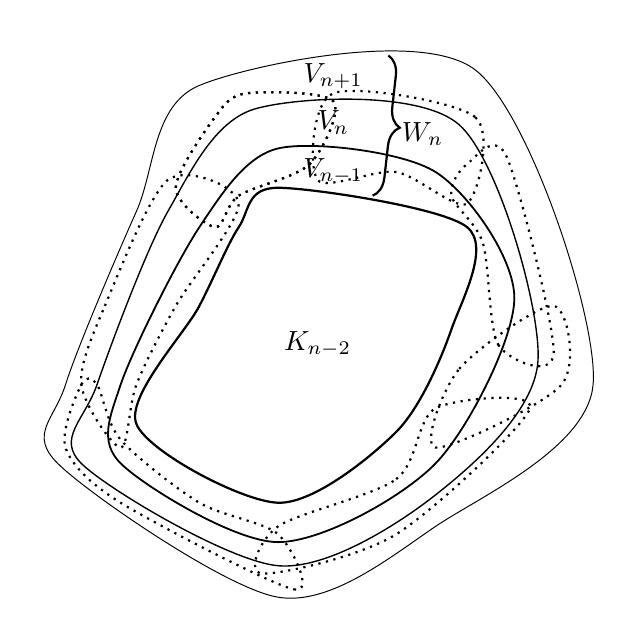
\begin{tikzpicture}
        \draw[line width=0.35] plot[smooth cycle] coordinates {
            (-0.8,1) (2,-0.7) (4,0.2) (6,2) (4.5,6) (1,5.8) (0.2,4.2) (-0.7,2)
        };
        \draw[line width=0.5] plot[smooth cycle] coordinates {
            (-0.5,1) (2,-0.3) (4,0.6) (5.3,2.3) (4.3,5.3) (1.7,5.5) (0.6,4.2) (-0.3,2)
        };
        \draw[line width=0.65] plot[smooth cycle] coordinates {
            (0,1) (2,0) (4,1) (5,3.1) (4,4.7) (2,5) (1,4) (0,2)
        };
        \draw[thick] plot[smooth cycle] coordinates {
            (0.2,1.5) (2,0.5) (3.5,1.4) (4.2,2.7) (4.4,4) (2,4.5) (1.5,4) (1,3)
        };
        \draw[thick, dotted] plot[smooth cycle] coordinates {
            (4.4,4.3) (4.5,5.4) (2.7,5.7) (2.5,4.6) (3.5,4.7)
        };
        \draw[thick, dotted] plot[smooth cycle] coordinates {
            (1.2,4) (0.7,4.5) (1.2,5.4) (1.6,5.7) (2.7,5.6) (2.4,4.8) (1.5,4.4)
        };
        \draw[thick, dotted] plot[smooth cycle] coordinates {
            (1.2,4) (0.7,4.5) (1.2,5.4) (1.6,5.7) (2.7,5.6) (2.4,4.8) (1.5,4.4)
        };
        \draw[thick, dotted] plot[smooth cycle] coordinates {
            (-0.5,2) (-0.2,3) (0.6,4.6) (1.5,4.3) (0.7,3) (0.2,2) (0,1.2)
        };
        \draw[thick, dotted] plot[smooth cycle] coordinates {
            (0,0.5) (2.2,-0.6) (2,0.1) (1,0.5) (0,1.3) (-0.3,2) (-0.5,2) (-0.7,1.2)
        };
        \draw[thick, dotted] plot[smooth cycle] coordinates {
            (2,0.2) (3.5,0.8) (4,1.7) (5.2,1.7) (3.5,0.1) (1.8,-0.4)
        };
        \draw[thick, dotted] plot[smooth cycle] coordinates {
            (4,1.2) (4.3,2.2) (5.5,3) (5.6,2)
        };
        \draw[thick, dotted] plot[smooth cycle] coordinates {
            (5.5,2.4) (4.8,2.5) (4.6,3.8) (4.2,4.4) (4.4,4.8) (4.9,4.9)
        };

        \node[anchor=north] at (2.5,2.8) {\(K_{n-2}\)};
        \node[anchor=north] at (2.7,5) {\(V_{n-1}\)};
        \node[anchor=north] at (2.7,5.6) {\(V_n\)};
        \node[anchor=north] at (2.7,6.2) {\(V_{n+1}\)};
        \draw[decorate,decoration={brace, amplitude=7pt}, thick] (3.4,6.18) -- (3.2,4.4) node[midway, yshift=-3pt, right=4pt] {\(W_n\)};
    \end{tikzpicture}
    \caption{The geometry of the finite subcover of \(V_n\subset W_n\) for some \(n\in\mathbb{N}\).}
    \label{fig:locallyfiniteopencoverexistence}
\end{figure}
\begin{remark}
    The property of local finiteness of an open collection \(S\) in \(\Omega\) is commonly stated as: for every \(z\in\Omega\), there exists an open neighborhood of \(z\) that intersects only finitely many sets in \(S\).

    This is equivalent to
    \cref{itm:locallyfiniteopencoverexistence_localfiniteness} in
    \cref{lem:locallyfiniteopencoverexistence}. Indeed, if every point has such a
    neighborhood, then any compact \(K\subset\Omega\) admits a finite subcover of
    these neighborhoods by Heine--Borel (\cref{thm:heineborel}), so \(K\)
    intersects finitely many sets in \(S\). Conversely, for any \(z\in\Omega\),
    take an open neighborhood \(V\ni z\) with relatively compact closure in
    \(\Omega\); then \(\overline{V}\) intersects finitely many sets in \(S\), and
    so does \(V\).
\end{remark}
\begin{theorem}[Partition of Unity]\label{thm:partitionofunity}
    Let \(\Omega\subseteq\mathbb{C}\) be a nonempty open set and let \(\cbraces{\Omega_k}_{k\in\mathbb{N}}\) be an open cover of \(\Omega\). Then there exists a collection of bump functions \(\cbraces{\alpha_j}_{j\in\mathbb{N}}\subset C^\infty(\mathbb{C})\), each with compact support in \(\Omega\), satisfying:
    \begin{enumerate}
        \item For each \(j\in\mathbb{N}\), there exists \(k\in\mathbb{N}\) such that
            \(\supp\qty(\alpha_j)\subseteq\Omega_k\).\label{itm:partitionofunity_subordinate}
        \item The collection \(\cbraces{\supp\qty(\alpha_j)}_{j\in\mathbb{N}}\) is locally
            finite.\label{itm:partitionofunity_localfiniteness}
        \item For each \(j\in\mathbb{N}\), \(0\le\alpha_j\le1\).
            \label{itm:partitionofunity_nonnegativity}
        \item \(\sum_{j=1}^\infty\alpha_j\equiv1\) on \(\Omega\).\label{itm:partitionofunity_partitionofunity}
    \end{enumerate}
    This is called a \(C^\infty\) partition of unity \textscsl{subordinate to} \(\cbraces{\Omega_k}_{k\in\mathbb{N}}\).
\end{theorem}
\begin{proof}
    For each \(z\in\Omega\) there exists \(r_z>0\) and \(k_z\in\mathbb{N}\) such that \(\overline{D\qty(z,r_z)}\subset\Omega_{k_z}\). The collection \(\cbraces{D(z,r)}{z\in\Omega\wedge0<r<r_z}\) is an open basis for \(\Omega\). By \cref{lem:locallyfiniteopencoverexistence} there exists a locally finite open cover \(\cbraces{D\qty(z_j,r_{z_j})}_{j\in\mathbb{N}}\subseteq\mathfrak{B}\) of \(\Omega\) with
    \[D\qty(z_j,r_{z_j})\subset\overline{D\qty(z_j,r_{z_j})}\subset\Omega_{k_{z_j}},\quad\forall j\in\mathbb{N}.\]
    Define the standard bump function
    \[\theta(z)=
        \begin{dcases}
            \exp\qty(\frac{1}{\abs{z}^2-1}) & \qif*\abs{z}<1,   \\
            0                               & \qif*\abs{z}\ge1.
    \end{dcases}\]
    For \(\varepsilon>0\) let
    \(\theta_\varepsilon(z)=\varepsilon^{-2}\theta\qty(\frac z\varepsilon)\), which
    has support \(\overline{D(0,\varepsilon)}\) and satisfies \[\int_{\mathbb{C}}\theta_\varepsilon(z)\ddx\wedge\ddy=1.\]
    Define \(\beta_j(z)=\theta_{r_{z_j}}\qty(z-z_j)\), so
    \(\supp(\beta_j)=\overline{D\qty(z_j,r_{z_j})}\subset\Omega_{k_{z_j}}\).

    By local finiteness of \(\cbraces{D\qty(z_j,r_{z_j})}_{j\in\mathbb{N}}\), for
    each \(z\in\Omega\) there exists an open neighborhood \(V\ni z\) intersecting
    only finitely many \(\overline{D\qty(z_j,r_{z_j})}\). Thus
    \(\cbraces{\supp(\beta_j)}_{j\in\mathbb{N}}\) is locally finite on \(\Omega\).
    Then the sum \(S(z)=\sum_{j=1}^\infty\beta_j(z)\) defined for \(z\in\Omega\)
    involves only finitely many nonzero terms (by local finiteness) on a
    neighborhood of every point \(z\). Hence \(S\in C^\infty(\Omega)\) and
    \(S(z)>0\) (since \(\cbraces{D\qty(z_j,r_{z_j})}_{j\in\mathbb{N}}\) covers
    \(\Omega\)). Define
    \[\alpha_j(z)=\frac{\beta_j(z)}{S(z)},\quad\forall j\in\mathbb{N}.\]
    Each \(\alpha_j\in C^\infty(\mathbb{C})\) has compact support in \(\Omega\),
    \(0\le\alpha_j\le1\), the supports are locally finite, and
    \(\sum_{j=1}^\infty\alpha_j(z)=1\) for all \(z\in\Omega\). Moreover
    \(\supp(\alpha_j)\subseteq\Omega_{k_{z_j}}\), proving subordination.
\end{proof}
\begin{theorem}[Existence of Bump Functions]\label{thm:bumpfunctionexistence}
    Let \(K\subset\mathbb{C}\) be compact and \(V\subset\mathbb{C}\) an open neighborhood of \(K\). Then there exists a compactly supported \(\varphi\in C^\infty(\mathbb{C})\) such that
    \[0\leq\varphi(z)\leq1\quad\forall z\in\mathbb{C},\]
    \(\supp(\varphi)\subset V\), and \(\varphi\equiv1\) on some open neighborhood of \(K\).
\end{theorem}
\begin{proof}
    Let \(V(K,\varepsilon)=\cbraces{z\in\mathbb{C}}{\inf_{\zeta\in K}\abs{z-\zeta}<\varepsilon}\) denote the open \(\varepsilon\)-neighborhood of \(K\). Since \(V\) is an open neighborhood of \(K\), \(\exists\varepsilon>0\) such that
    \[K\subset V(K,\varepsilon)\subset V(K, 2\varepsilon)\subset V,\]
    where \(A\subset\subset B\) means that the closure of \(A\) is compact and
    contained in \(B\).

    Define the open sets
    \[\Omega_1=V(K,2\varepsilon),\qquad\Omega_2=\mathbb{C}\setminus\overline{V(K,\varepsilon)}.\]
    Then \(\cbraces{\Omega_1,\Omega_2}\) is an open cover of \(\mathbb{C}\).

    By the Partition of Unity Theorem (\cref{thm:partitionofunity}), there exist
    compactly supported functions \(\cbraces{\alpha_j}_{j\in\mathbb{N}}\subset
    C^\infty(\mathbb{C})\) forming a partition of unity subordinate to this cover.
    That is,
    \[0\leq\alpha_j\leq1,\quad\supp\qty(\alpha_j)\subset\Omega_{i_j}\text{ for some }i_j\in\cbraces{1,2},\quad\sum_{j=1}^\infty\alpha_j\equiv1\qq{on}\mathbb{C}.\]
    Define
    \[\varphi(z)=\sum_{\substack{j\in\mathbb{N}\\\supp\qty(\alpha_j)\subset\Omega_1}}\alpha_j(z).\]
    Then \(\varphi\in C^\infty(\mathbb{C})\) is compactly supported within
    \(\Omega_1\), and since only finitely many \(\alpha_j\) are nonzero on a
    neighborhood of each point, \(\varphi\in C^\infty(\mathbb{C})\). Moreover,
    \(\supp(\varphi)\subset\Omega_1\subset V\).

    For \(z\in V(K,\varepsilon)\), all functions with support in \(\Omega_2\)
    vanish at \(z\), so
    \[\varphi(z)=\sum_{\supp\qty(\alpha_j)\subset\Omega_1}\alpha_j(z)=\sum_{j=1}^\infty\alpha_j(z)=1.\]
    Hence, \(\varphi\equiv 1\) on the open neighborhood \(V(K,\varepsilon)\) of
    \(K\). Outside \(V(K,2\varepsilon)\), all terms with support in \(\Omega_1\)
    vanish, so \(\varphi(z)=0\). Finally, \(0\leq\varphi\leq1\) everywhere by
    construction.

    Thus \(\varphi\) satisfies all required properties.
\end{proof}
\subsection{Zeros of a Holomorphic Function}
For a region \(U\subseteq\mathbb{C}\) and a holomorphic function
\(f:U\to\mathbb{C}\), a point \(z_0\in U\) is a \textscsl{zero} of \(f\) iff
\(f\paren{z_0}=0\). Furthermore, if \(f\) has the Taylor expansion at \(z_0\)
of \[a_m\paren{z-z_0}^m+a_{m+1}\paren{z-z_0}^{m+1}+\cdots,\qquad m\in\mathbb{N},a_m\neq0,\] then the zero at \(z_0\) has multiplicity \(m\).

We will introduce a fundamental application of Liouville's Theorem
(\cref{thm:liouville}) below.
\begin{theorem}[Fundamental Theorem of Algebra]\label{thm:fundamentaltheoremofalgebra}
    Every non-constant polynomial \(p(z)\) with complex coefficients has at least one complex zero.
\end{theorem}
\begin{proof}
    For the sake of contradiction, suppose that \(p(z)\) has no complex zeros. Then the function \(f(z)=\frac{1}{p(z)}\) is continuous and entire, because \(p(z)\) has no zeros in \(\mathbb{C}\). Moreover, as \(z\to\infty\), \(p(z)\to\infty\), so \(f(z)\to 0\), and thus \(f(z)\) is bounded. By Liouville's Theorem (\cref{thm:liouville}), every bounded entire function is constant. Thus, \(f(z)\) is constant, and so \(p(z)\) must also be constant. By contradiction, \(p(z)\) has at least one complex zero.
\end{proof}
\begin{theorem}\label{thm:identityaccumulationofzeros}
    Let \(U\subseteq\mathbb{C}\) be open and connected, and \(f:U\to\mathbb{C}\) be holomorphic over \(U\). Then if the set defined by \(S=\cbraces{z\in U}{f(z)=0}\) has an accumulation point in \(U\), then \(f\equiv0\) over \(U\).
\end{theorem}
\begin{proof}
    Let \(\cbraces{z_n}_{n\in\mathbb{N}}\) be a subset of \(S\) and assume it has an accumulation point \(z_\infty\) in \(U\). Since \(f\) is holomorphic over \(U\), \(\exists\varepsilon>0\) such that \(f\) is holomorphic over \(D\paren{z_\infty,\varepsilon}\subseteq U\). Then over this disk, \(f\) has the Taylor expansion
    \begin{equation}\label{eq:identityaccumulationofzeros_taylorexpansion}
        f(z)=\sum_{n=0}^\infty a_n\paren{z-z_\infty}^n.
    \end{equation}
    By \cref{def:accumulationpoint}, \(\exists N\in\mathbb{N}\) such that \(\forall n>N\), \(z_n\in D\paren{z_\infty,\varepsilon}\). Since \(z_n\) is a zero of \(f\), \(f\paren{z_n}=0\). Then, by the continuity of \(f\), \[\lim_{n\to\infty} f\paren{z_n}=f\paren{\lim_{n\to\infty}z_n}=f\paren{z_\infty}=0.\] Using this result in comparison to
    \cref{eq:identityaccumulationofzeros_taylorexpansion}, we get that \(a_0=0\).

    The function \(f_1(z)=\frac{f(z)}{z-z_\infty}\) has a Taylor expansion over
    \(D\paren{z_0,\varepsilon}\) of
    \[f_1(z)=\sum_{n=0}^\infty a_{n+1}\paren{z-z_\infty}^n.\]
    Let \(z=z_n\neq z_\infty\) for some \(n>N\). Then \(f_1\) vanishes, leaving \[0=a_1+\order{z_n-z_\infty}.\]
    Letting \(n\to\infty\), \(z_n\to z_\infty\), and \(a_1=0\). Define
    \(f_2(z)=\frac{f_1(z)}{z-z_\infty}\). Then, \[f_2(z)=\sum_{n=0}^\infty a_{n+2}\paren{z-z_\infty}^n.\]
    Similarly, \(a_2=0\). Letting \(f_n(z)=\frac{f(z)}{\paren{z-z_\infty}^n}\), the
    sequence \(\cbraces{a_n}_{n\in\mathbb{Z}_{\geq0}}\) vanishes, and \(f\equiv 0\)
    on \(D\paren{z_\infty,\varepsilon}\).

    Let \(\widetilde{S}=\cbraces{z\in U}{\forall n\in\mathbb{Z}_{\geq0},
    f^{(n)}(z)=0}\).\ \(\forall z\in D\paren{z_\infty,\varepsilon}\), since
    \(f(z)\) locally vanishes (and has vanishing derivatives as a consequence),
    \(D\paren{z_\infty,\varepsilon}\subseteq\widetilde{S}\). Furthermore, \(\forall
    z'\in\widetilde{S}\), \(\exists\varepsilon'>0\) such that \(f(z)\) has a
    convergent Taylor series with vanishing coefficients on
    \(D(z',\varepsilon')\subseteq U\). Then \(f\equiv0\) on
    \(D\paren{z',\varepsilon'}\). Then \(\forall z\in D(z',\varepsilon')\), since
    \(f\) is constant at \(z\), it also has vanishing derivatives. It follows that
    \(D(z',\varepsilon')\subseteq\widetilde{S}\). Since every point in
    \(\widetilde{S}\) has an open neighborhood also in \(\widetilde{S}\),
    \(\widetilde{S}\) is open.

    It is evident that \(\forall k\in\mathbb{Z}_{\geq0}\), \(f^{(k)}\) is
    continuous in \(U\) by the holomorphy of \(f\). Let \(S_k=\cbraces{z\in
    U}{f^{(k)}(z)=0}\). For any sequence \(\cbraces{\widetilde{z}_n}\in S_k\)
    converging to some \(\widetilde{z}_\infty\in U\), by the continuity of \(f\), \[\lim_{n\to\infty} f^{(k)}\paren{\widetilde{z}_n}=f^{(k)}\paren{\lim_{n\to\infty}\widetilde{z}_n}=f^{(k)}\paren{z'_\infty}=0,\] and therefore \(\widetilde{z}_\infty\in S_k\). Thus, \(S_k\) contains all of
    its accumulation points in \(U\) and is therefore closed in \(U\) (if
        \(\widetilde{z}_\infty\notin U\), then it is no longer relevant; we are
    concerned about it being closed within \(U\)). Since
    \(\widetilde{S}=\bigcap_{k\in\mathbb{Z}_{\geq0}} S_k\) and each of \(S_k\) is
    closed in \(U\), \(\widetilde{S}\) is the intersection of closed sets and
    consequently closed.

    Since \(\widetilde{S}\) is nonempty and clopen in the connected set \(U\),
    \(\widetilde{S}=U\) (by \cref{thm:connectedtopologicalspaceclopensets}). It
    follows that \(f\equiv 0\) on \(U\).
\end{proof}
\begin{remark}
    This is a trivial property of holomorphic functions that allows for the uniqueness of analytic continuations. It is oftentimes stated in the form below:
\end{remark}
\begin{theorem}[Identity Theorem]\label{thm:identity}
    Let \(U\subseteq\mathbb{C}\) be open and connected, and define \(f(z)\) and \(g(z)\) to be two holomorphic functions on \(U\). For a set \(S\subseteq U\) with an accumulation point in \(U\), if \(f\equiv g\) on \(S\), then \(f\equiv g\) on \(U\).
\end{theorem}
\begin{proof}
    Let \(h=f-g\) be holomorphic over \(U\). Since \(S\) has an accumulation point in \(U\), and \(h\equiv 0\) over \(S\), then by \cref{thm:identityaccumulationofzeros}, \(h\equiv 0\) over \(U\).
\end{proof}
\begin{theorem}[Holomorphic Argument Principle]\label{thm:argumentprincipleholomorphic}
    Let \(U\subseteq\mathbb{C}\) be a region and \(f:U\to\mathbb{C}\) be holomorphic. Let \(\gamma\subset U\) be a simple, closed, positively oriented curve that is null-homotopic in \(U\). If \(f\) has no zeros on \(\gamma\), then \(f\) has finitely many zeros in the region bounded by \(\gamma\), and this number, counting multiplicities, is given by
    \[k=\frac{1}{2\piup\ii}\oint_{\gamma}\frac{f'(z)}{f(z)}\ddz.\]
    Let \(\Gamma\) be the image of \(\gamma\) under the map \(w=f(z)\). Then
    \(k=\frac{1}{2\piup}\Delta_\Gamma\arg(w)\), where \(\Delta_\Gamma\arg(w)\)
    denotes the total change in argument of \(w\) as it traverses \(\Gamma\).
\end{theorem}
\begin{proof}
    Let \(z_1,\ldots,z_n\) be the distinct zeros of \(f\) enclosed by \(\gamma\) with the respective multiplicities \(k_1,\ldots,k_n\). Choose disjoint disks \(D\qty(z_j,\varepsilon_j)\) centered at each \(z_j\) with radii \(\varepsilon_j>0\), each contained in the interior of \(\gamma\) and avoiding \(\gamma\). The function \[\frac{f'(z)}{f(z)}\]
    is holomorphic on the domain \[\mathrm{int}\paren{\gamma}\setminus\bigcup_{j=1}^n\overline{D\qty(z_j,\varepsilon_j)},\]
    where \(\mathrm{int}(\gamma)\) denotes the interior relative to \(\gamma\). The
    oriented boundary of this domain is \(\gamma^+\cup\bigcup_{j=1}^n\partial
    D\paren{z_j,\varepsilon_j}^-\). By Cauchy--Goursat
    (\cref{thm:cauchygoursattheorem}),
    \[\int_{\gamma^+\cup\bigcup_{j=1}^n\partial D\paren{z_j,\varepsilon_j}^-}\frac{f'(z)}{f(z)}\ddz=0,\]
    which rearranges to
    \[\oint_{\gamma^+}\frac{f'(z)}{f(z)}\ddz=\sum_{j=1}^n\oint_{\partial D\paren{z_j,\varepsilon_j}^+}\frac{f'(z)}{f(z)}\ddz.\]
    Near each \(z_j\), express \(f(z)=\paren{z-z_j}^{k_j}h_j(z)\) where \(h_j\) is
    holomorphic and non-vanishing on \(D\paren{z_j,\varepsilon_j}\).
    Differentiation yields
    \[f'(z)=k_j\paren{z-z_j}^{k_j-1}h_j(z)+\paren{z-z_j}^{k_j}h_j'(z),\] and thus
    \[\frac{f'(z)}{f(z)}=\frac{k_j}{z-z_j}+\frac{h_j'(z)}{h_j(z)}.\]
    Since \(h_j\) is holomorphic and non-vanishing on
    \(D\paren{z_j,\varepsilon_j}\), the function \(\frac{h_j'}{h_j}\) is
    holomorphic there. By the Cauchy--Goursat Theorem,
    \[\oint_{\partial D\paren{z_j,\varepsilon_j}}\frac{h_j'(z)}{h_j(z)}\ddz=0.\]
    The Cauchy--Goursat Formula (\cref{thm:cauchygoursatformula}) gives
    \[\oint_{\partial D\paren{z_j,\varepsilon_j}}\frac{k_j}{z-z_j}\ddz=2\piup\ii k_j.\]
    Combining results,
    \[\oint_{\gamma}\frac{f'(z)}{f(z)}\ddz=\sum_{j=1}^n2\piup\ii k_j=2\piup\ii k.\]
    Finally, parameterize \(\Gamma\) by \(w=f(z)\). Then \(\dd{w}=f'(z)\ddz\), and
    \[k=\frac{1}{2\piup\ii}\oint_{\Gamma}\frac{\dd{w}}{w}=\frac{1}{2\piup\ii}\Delta_\Gamma\log(w)=\frac{1}{2\piup}\Delta_\Gamma\arg(w),\] which proves the result.
\end{proof}
Thus, one defines the \textscsl{winding index} to quantify how many times a closed curve winds counterclockwise around a given point in the complex plane. Formally, if \(\gamma=\gamma([0,1])\) is a counterclockwise-oriented closed curve and \(z\) is a point satisfying \(z\notin\gamma\), then \[\mathrm{Ind}_{\gamma}(z)=\frac{1}{2\piup\ii}\int_\gamma\frac{\ddzeta}{\zeta-z}=\frac{1}{2\piup\ii}\int_0^1\frac{\gamma'(t)\ddt}{\gamma(t)-z}.\]
\begin{theorem}\label{thm:hurwitzsimplecase}
    Let \(\cbraces{f_n(z)}\) be a sequence of holomorphic functions on the open set \(U\subseteq\mathbb{C}\) that uniformly converges to \(f(z)\) on every compact subset of \(U\). If \(\forall n\in\mathbb{N}\), \(f_n(z)\) has no zeros in \(U\), then \(f\) is either identically 0 or has no zeros in \(U\).
\end{theorem}
\begin{proof}
    By the holomorphy of \(f_n(z)\), for any simple closed rectifiable curve \(\gamma\subset U\) (whose interior is a subset of \(U\)), by the Cauchy--Goursat Theorem (\cref{thm:cauchygoursattheorem}), \[\oint_{\gamma}f_n(\zeta)\ddzeta=0.\] Since \(\gamma\) is a subset of any compact subset of \(U\),
    \(\cbraces{f_n(\zeta)}\) uniformly converges on \(\gamma\), and by
    \cref{thm:limitintegralswitch},
    \begin{equation}
        \lim_{n\to\infty}\oint_{\gamma}f_n(\zeta)\ddzeta=\oint_{\gamma}\lim_{n\to\infty}f_n(\zeta)\ddzeta=\oint_{\gamma}f(\zeta)\ddzeta=0.\label{eq:hurwitzsimplecase_integrallimitswitchforholomorphy}
    \end{equation}
    Then by Morera's Theorem (\cref{thm:morera}), \(f(z)\) is holomorphic, and \(f'(z)\) is holomorphic. We aim to show that \(f'_n(z)\rightrightarrows f'(z)\).

    Let \(K\subset U\) be arbitrary and compact and \(V\supset K\) be open and
    relatively compact in \(U\). Since \(\cbraces{f'_n(z)}\) is holomorphic, by
    \cref{cor:nthderivativeboundedsupremum}, there exists a finite constant \(c>0\)
    such that \[\lim_{n\to\infty}\sup_{z\in K}\abs{f'_n(z)-f'(z)}\leq c\lim_{n\to\infty}\sup_{z\in V}\abs{f_n(z)-f(z)}.\]

    By the definition of uniform convergence, the right-hand side approaches 0, and
    \(\cbraces{f'_n(z)}\) is then uniformly convergent to \(f'(z)\) by the same
    reasoning.

    Through the proof of \cref{thm:identityaccumulationofzeros}, if
    \(f\not\equiv0\) over \(U\), then the zeros of \(f\) do not have an
    accumulation point in \(U\) and are therefore discrete. In this case, let
    \(\gamma\subset U\) be a curve that does not pass through the zeros of \(f\).
    Since each function in the sequence \(f_n\) does not contain zeros in \(U\), by
    the Argument Principle, (\cref{thm:argumentprincipleholomorphic}),
    \begin{equation}
        \lim_{n\to\infty}\oint_{\gamma}\frac{f_n'(z)}{f_n(z)}\ddz=0.\label{eq:hurwitzsimplecase_argumentprinciple}
    \end{equation}
    Since \(f\) and \(f'\) are holomorphic over \(\gamma\), by \cref{thm:continuousfunctionboundedoncompact}, there exists a finite value \(M>0\) such that \(\forall z\in\gamma\), \(\max\cbraces{\abs{f(z)},\abs{f'(z)}}<M\).

    Since \(\gamma\) does not pass through the zeros of \(f\), \(\exists\lambda>0\)
    such that \(\forall z\in\gamma\), \(\abs{f(z)}>\lambda\). By the uniform
    convergence of \(\cbraces{f_n(z)}\), \(\exists N\in\mathbb{N}\) such that
    \[\abs{f_n(z)-f(z)}<\frac{\lambda}{2},\quad\forall n>N,\forall z\in\gamma.\]
    Then \(\abs{f_n(z)}>\frac{\lambda}{2}\) on \(\gamma\). Hence,
    \(\frac{1}{f_n(z)}\) and its limit are uniformly bounded; \[\abs{\frac{1}{f(z)}}<\frac{1}{\lambda},\quad\abs{\frac{1}{f_n(z)}}<\frac{2}{\lambda},\quad\forall z\in\gamma,\forall n>N.\]
    Then,
    \begin{align*}
        \abs{\frac{f'}{f}-\frac{f'_n}{f_n}}                                               & =\abs{\frac{f'f_n-f'_n f}{f_n f}}                                                                       \\
        & <2\frac{\abs{f'f_n-f'f}+\abs{f'f-f'_n f}}{\lambda^2}                                                    \\
        & <\frac{2M}{\lambda^2}\cdot\paren{\abs{f_n-f}+\abs{f'-f'_n}}.                                            \\
        \sup_{z\in\gamma}\abs{\frac{f'(z)}{f(z)}-\frac{f'_n(z)}{f_n(z)}}                  & \leq\frac{2M}{\lambda^2}\paren{\sup_{z\in\gamma}\abs{f_n(z)-f(z)}+\sup_{z\in\gamma}\abs{f'(z)-f'_n(z)}} \\
        \lim_{n\to\infty}\sup_{z\in\gamma}\abs{\frac{f'(z)}{f(z)}-\frac{f'_n(z)}{f_n(z)}} & \leq\frac{2M}{\lambda^2}\paren{\lim_{n\to\infty}\sup_{z\in\gamma}\abs{f_n(z)-f(z)}+\abs{f'(z)-f'_n(z)}} \\
        & =0.
    \end{align*}
    Therefore, \(\frac{f'(z)}{f(z)}\) is uniformly convergent on \(\gamma\). By \cref{thm:limitintegralswitch}, we can pass the limit through the integral in \cref{eq:hurwitzsimplecase_argumentprinciple}. Then,
    \[\lim_{n\to\infty}\oint_\gamma\frac{f'_n(z)}{f_n(z)}\ddz=\oint_\gamma\frac{f'(z)}{f(z)}\ddz=0.\] By the Argument Principle, (\cref{thm:argumentprincipleholomorphic}), \(f(z)\)
    has no zeros in the interior of \(\gamma\). Since \(\gamma\) was arbitrarily
    chosen, either \(f(z)\equiv 0\) on \(U\) or has no zeros in \(U\).
\end{proof}
\begin{theorem}[\textsc{Rouché}]\label{thm:rouche}
    Let \(U\subseteq\mathbb{C}\) be open and \(f,g\) be two holomorphic functions over \(U\). Let \(\gamma\subset U\) be a simple, closed, rectifiable curve, and \(\forall z\in\gamma\)
    \begin{equation}
        \abs{f(z)-g(z)}<\abs{f(z)}\label{eq:rouche}.
    \end{equation} Then \(f\) and \(g\) have the same number of zeros enclosed by \(\gamma\) and do not vanish on \(\gamma\).
\end{theorem}
\begin{proof}
    It is obvious that \(g(z)\) has no zeros on \(\gamma\). Otherwise, \(\exists z_0\in\gamma\) such that \(g\paren{z_0}=0\), implying that \(\abs{f\paren{z_0}}<\abs{f\paren{z_0}}\) which is impossible. Similarly, \(f(z)\) has no zeros on \(\gamma\), since \(\abs{g(z)}<0\) is an impossibility.

    Let \(k_f\) and \(k_g\) denote the number of zeros of \(f\) and \(g\) enclosed
    by \(\gamma\), respectively. By the Argument Principle
    (\cref{thm:argumentprincipleholomorphic}),
    \begin{align*}
        k_g-k_f & =\int_{\gamma}\frac{g'(z)}{g(z)}\ddz-\int_\gamma\frac{f'(z)}{f(z)}\ddz                                                  \\
        & =\int_\gamma\frac{g'(z)f(z)-f'(z)g(z)}{g(z)f(z)}\ddz=\int_\gamma\frac{\qty(\frac{g(z)}{f(z)})'}{\frac{g(z)}{f(z)}}\ddz.
    \end{align*}
    Let \(w=h(z)=\frac{g(z)}{f(z)}\) with \(\Gamma=h(\gamma)\). Then, \[k_g-k_f=\int_\Gamma\frac{\dd{w}}{w}.\]
    From \cref{eq:rouche}, by dividing both sides by \(f(z)\), we obtain
    \(\abs{w-1}<1\). Then \(\Gamma\) lies in the open disk \(D(1,1)\), which will
    never intersect or enclose 0. Then by
    \cref{lem:cauchyintegraltheoremoversimplyconnectedset}, \[k_g-k_f=\int_\Gamma\frac{\dd{w}}{w}=0,\] as desired.
\end{proof}
By the Fundamental Theorem of Algebra (\cref{thm:fundamentaltheoremofalgebra}), any polynomial in the form \(p(z)=\sum_{k=0}^n a_kz^k\) (\(n\in\mathbb{N}\), \(a_n\neq 0\), \(a_k\in\mathbb{C}\) where \(k=1,\ldots n\)) has at least one complex zero. Consider the function \(q(z)=a_nz^n\), with a zero at \(z=0\) with multiplicity \(n\). By Rouché's Theorem (\cref{thm:rouche}), since \(\exists R\in\mathbb{R}\) such that \(\abs{q(z)-p(z)}=\abs{\sum_{k=0}^{n-1}a_k z^k}<\abs{a_n z^n}\) over \(\abs{z}=R\), \(p\) and \(q\) have the same number of zeros, counting multiplicity.
\begin{theorem}\label{thm:hurwitzshifts}
    Let \(U\subseteq\mathbb{C}\) be open and connected, and \(f(z)\) be holomorphic and non-constant on \(U\).

    If \(z_0\in U\) and \(w_0=f\qty(z_0)\), and the multiplicity of the zero at
    \(z_0\) of \(f-w_0\) is \(m\), then for all \(\rho>0\) such that \(f-w_0\) is
    non-vanishing on \(\overline{D\qty(z_0,\rho)}\setminus\cbraces{z_0}\),
    \(\exists\delta>0\) such that \(\forall\xi\in D\qty(w_0,\delta)\), \(f-\xi\)
    has \(m\) zeros in \(D\qty(z_0,\rho)\), counting multiplicity.
\end{theorem}
\begin{proof}
    The zero at \(z_0\) is isolated by \cref{thm:identityaccumulationofzeros}. Furthermore, \(\abs{f-w_0}\) is continuous on \(\partial D\qty(z_0,\rho)\) and attains a positive infimum \(\delta\). In other words, on this set, \(\abs{f-w_0}\geq\delta\). Hence, \(\forall\xi\in D\qty(w_0,\delta)\), we have \(\abs{\xi-w_0}<\delta\leq\abs{f(z)-w_0}\) for any \(z\in\partial D\qty(z_0,\rho)\).

    By Rouché's Theorem, since
    \(\abs{\qty(f(z)-w_0)-\qty(f(z)-\xi)}<\abs{f(z)-w_0}\), it follows that
    \(f-\xi\) and \(f-w_0\) have the same number of zeros in \(D\qty(z_0,\rho)\).
\end{proof}
We also have the following generalization of \cref{thm:hurwitzsimplecase}, which is a heuristic restatement of \cref{thm:hurwitzshifts}:
\begin{theorem}[\textsc{Hurwitz}]\label{thm:hurwitz}
    Let \(U\subseteq\mathbb{C}\) be an open and connected set, and suppose \(\cbraces{f_n(z)}_{n\in\mathbb{N}}\) is a holomorphic function sequence that uniformly converges to a non-constant function \(f(z)\) on all compact sets of \(U\).

    If \(z_0\in U\) and \(w_0=f\qty(z_0)\), and the multiplicity of the zero at
    \(z_0\) of \(f-w_0\) is \(m\), then for all \(\rho>0\) such that \(f-w_0\) is
    non-vanishing on \(\overline{D\qty(z_0,\rho)}\setminus\cbraces{z_0}\),
    \(\exists N\in\mathbb{N}\) such that \(\forall n>N\), \(f_n-w_0\) has \(m\)
    zeros in \(D\qty(z_0,\rho)\), counting multiplicity.
\end{theorem}
\begin{proof}
    The zero at \(z_0\) is isolated by \cref{thm:identityaccumulationofzeros}. Furthermore, \(\abs{f-w_0}\) is continuous on \(\partial D\qty(z_0,\rho)\) and attains a positive infimum \(\delta\). In other words, on this set, \(\abs{f-w_0}\geq\delta\). By uniform convergence, \(\exists N\in\mathbb{N}\) such that \(\forall n>N\), we have \(\abs{f(z)-f_n\qty(z)}<\delta\leq\abs{f(z)-w_0}\) for any \(z\in\partial D\qty(z_0,\rho)\).

    By Rouché's Theorem (\cref{thm:rouche}), since \[\abs{\qty(f(z)-w_0)-\qty(f_n(z)-w_0)}<\abs{f(z)-w_0},\] it follows that \(f_n-w_0\) and \(f-w_0\) have the same number of zeros in
    \(D\qty(z_0,\rho)\).
\end{proof}
\subsection{Further Properties of Holomorphic Functions}
A useful corollary of \cref{thm:cauchygoursatformula} is the Maximum Modulus
Principle.

Before the theorem, we first introduce the mean-value property of holomorphic
functions.
\begin{lemma}\label{lem:holomorphicmeanvalueproperty}
    Let \(U\subseteq\mathbb{C}\) be open and simply connected, and let \(f:U\to\mathbb{C}\) be holomorphic. Then \(\forall z\in U\) and \(\forall\varepsilon>0\) such that \(\overline{D(z,\varepsilon)}\subset U\), \(f(z)\) is the average of \(f(\zeta)\) where \(\zeta\in D(z,\varepsilon)\) is uniform. In other words, \[f(z)=\frac{1}{2\piup\varepsilon}\oint_{\partial D(z,\varepsilon)}f(\zeta)\abs{\dd{\zeta}}.\]
\end{lemma}
\begin{proof}
    By the Cauchy--Goursat Formula (\cref{thm:cauchygoursatformula}), \[f(z)=\frac{1}{2\piup\ii}\oint_{\partial D(z,\varepsilon)}\frac{f(\zeta)}{\zeta-z}\ddzeta=\frac{1}{2\piup}\int_0^{2\piup}f\paren{z+\varepsilon\ee^{\ii t}}\dd{t}.\]
    Observe that
    \begin{align*}
        f(z)=\frac{1}{2\piup\varepsilon}\oint_{\partial D(z,\varepsilon)}f(\zeta)\abs{\dd{\zeta}} & =\frac{1}{2\piup\varepsilon}\int_{0}^{2\piup}f\paren{z+\varepsilon\ee^{\ii t}}\abs{\ii\varepsilon\ee^{\ii t}\dd{t}} \\
        & =\frac{1}{2\piup}\int_{0}^{2\piup}f\paren{z+\varepsilon\ee^{\ii t}}\dd{t},
    \end{align*}
    and the conclusion follows.
\end{proof}
Since the real and imaginary parts of holomorphic functions are real-valued harmonic functions, they also satisfy the mean-value property. Furthermore, if a real continuous function satisfies the mean-value property, it is harmonic (to be proved in \cref{thm:meanvaluepropertysolutionsareharmonic}). This equivalence allows for the alternative definition of harmonic functions.
\begin{theorem}[Maximum Modulus Principle]\label{thm:maximummodulus}
    Let \(f(z)\) be holomorphic on an open connected region \(U\subseteq\mathbb{C}\). If \(\exists z_0\in U\) and an open neighborhood \(V\subseteq U\) of \(z_0\) such that \(\forall z\in V\), \(\abs{f\paren{z_0}}\geq\abs{f(z)}\), then \(f\) is a constant function on \(U\).
\end{theorem}
\begin{proof}
    Assume that \(z_0\) exists. We will first prove that the set \[S=\cbraces{z}{f(z)=f\paren{z_0},z\in V}\]
    is all of \(V\). This is equivalent to proving that \(S\) is nonempty, open,
    and closed in \(V\).

    Since \(z_0\in S\), the first condition is satisfied (nonemptiness). For any
    sequence \(\cbraces{z_n}\in S\) converging to some \(z_\infty\in V\), by the
    continuity of \(f\), \[\lim_{n\to\infty} f\paren{z_n}=f\paren{\lim_{n\to\infty}z_n}=f\paren{z_\infty}=0,\] and \(z_\infty\in S\). Thus, \(S\) contains all of its accumulation points in
    \(V\) and is therefore closed (if \(z_\infty\notin V\), then it is no longer
    relevant; we are concerned with its relative closedness in \(V\)).

    Since \(S\subseteq V\) and \(V\) are both open, \(\forall z\in S\),
    \(\exists\lambda>0\) such that \(D(z,\lambda)\subseteq V\). By
    \cref{lem:holomorphicmeanvalueproperty}, \(\forall 0<\varepsilon<\lambda\),
    \begin{align*}
        |f(z)| & =\abs{\frac{1}{2\piup}\int_0^{2\piup}f\paren{z+\varepsilon\ee^{\ii t}}\dd{t}}\leq\frac{1}{2\piup}\int_0^{2\piup}\abs{f\paren{z+\varepsilon\ee^{\ii t}}}\dd{t} \\
        & \leq\frac{1}{2\piup}\int_0^{2\piup}\abs{f(z)}\dd{t}=\abs{f(z)}.
    \end{align*}
    It follows that all inequalities above are equalities, or that
    \begin{align*}
        |f(z)| & =\abs{\frac{1}{2\piup}\int_0^{2\piup}f\paren{z+\varepsilon\ee^{\ii t}}\dd{t}}=\frac{1}{2\piup}\int_0^{2\piup}\abs{f\paren{z+\varepsilon\ee^{\ii t}}}\dd{t} \\
        & =\frac{1}{2\piup}\int_0^{2\piup}\abs{f(z)}\dd{t}=\abs{f(z)}.
    \end{align*}
    From the equality of the last two integrals, \(\int_{0}^{2\piup}\qty(\abs{f(z)}-\abs{f\paren{z+\varepsilon\ee^{\ii t}}})\dd{t}=0\). Since this integrand is strictly non-negative, we have equality. Thus, \(\forall z\in S\), \(\exists\lambda>0\) such that \(D\paren{z,\lambda}\subseteq S\). In other words, every \(z\in S\) has an open neighborhood that also lies in \(S\). Therefore, \(S\) is open and \(S=V\) as it is a nonempty clopen subset. Since \(V\) is nonempty and open, it has an accumulation point in \(U\). It follows that \(f(z)\equiv f\paren{z_0}\) over \(U\) by the Identity Theorem (\cref{thm:identity}).
\end{proof}
\begin{remark}
    If \(f\) is holomorphic and non-constant on an open region \(U\subseteq\mathbb{C}\), then for any compact set \(K\subset U\), the maximum of \(f\) in \(K\) lies on \(\partial K\). Otherwise, \(f\) would attain a maximum at some \(z\in\interior{K}\), and contradict the statement of \cref{thm:maximummodulus} under the assumption of being non-constant.
\end{remark}
A similar theorem exists for real-valued harmonic functions. The proof follows in the same way as the one for holomorphic functions. We will state it formally below.
\begin{theorem}\label{thm:maximumprincipleforrealharmonicfunctions}
    Let \(U\subseteq\mathbb{C}\) be open and connected and let \(f:U\to\mathbb{R}\) be harmonic. Suppose that \(\exists z_0\in U\) and a neighborhood \(V\subseteq U\) of \(z_0\) such that either \[f(z)\geq f\qty(z_0)\quad\forall z\in V\qq{or}f\qty(z_0)\quad\forall z\in V.\]
    Then \(f\) is constant on \(U\).
\end{theorem}
By nature of the proof, the result holds for any continuous function satisfying the mean-value property.
\subsection{The Group of Holomorphic Automorphisms on the Unit Disk}
The following important result can be directly obtained from the Maximum
Modulus Principle.
\begin{lemma}[Schwarz]\label{lem:schwarz}
    If \(f:\mathbb{D}\to\mathbb{D}\) is holomorphic and \(f(0)=0\), then \[\abs{f(z)}\leq\abs{z},\quad\abs{f'(0)}\leq 1.\]
    Any one of the inequalities becomes equalities iff \(f(z)\) is in the form of
    \(z\ee^{\ii\tau}\), where \(\tau\in\mathbb{R}\). In other words, \(f\) is a
    pure rotation.
\end{lemma}
\begin{proof}
    Define the auxiliary function \[g(z)=
        \begin{dcases}
            \frac{f(z)}{z} & \qif* z\neq0, \\
            f'(0)          & \qif* z=0.
    \end{dcases}\]
    Because \(\lim_{z\to0}\frac{f(z)}{z}=f'(0)\), \(g(z)\) is holomorphic on
    \(\mathbb{D}\). Since \(f\) is an automorphism on the open disk,
    \(\forall\abs{z}<1\), \(\abs{f(z)}<1\). By the Maximum Modulus Principle
    \cref{thm:maximummodulus}, \(\forall0<\varepsilon<1\), \(\forall z\in
    D(0,\varepsilon)\), \[\abs{g(z)}\leq\max_{z_\varepsilon\in\partial D(0,\varepsilon)}\frac{\abs{f\paren{z_\varepsilon}}}{\varepsilon}<\frac{1}{\varepsilon}.\] As \(\varepsilon\to 1^-\), we obtain that \(\forall z\in\mathbb{D}\),
    \(\abs{g(z)}\leq 1\), or that \(\abs{f(z)}\leq\abs{z}\). Let \(z=0\). Then we
    get \(\abs{g(0)}=f'(0)\leq 1\).

    For the sake of the equality condition, assume \(\abs{f(z)}=\abs{z}\). Then
    \(\abs{g(z)}\equiv 1\) on the unit open disk. By \cref{thm:maximummodulus},
    \(g(z)=\exp(\ii\tau)\) where \(\tau\in\mathbb{R}\) and \(f(z)=z\exp(\ii\tau)\)
    on \(\mathbb{D}\).

    Next, assume only that \(\abs{f'(0)}=1\). It follows that \(\abs{g(0)}=1\).
    Since \(\abs{g(z)}\leq 1\) for all \(z\in\mathbb{D}\), it follows from
    \cref{thm:maximummodulus} that \(g\) is constant with magnitude 1, or in the
    form of \(\exp(\ii\tau)\), where \(\tau\in\mathbb{R}\) is a constant.
    Consequently, \(f(z)=z\exp(\ii\tau)\).
\end{proof}
To discuss the main topic of this section, we will first introduce the concept of a \textscsl{group}.
\begin{definition}[Group]\label{def:group}
    A group is a nonempty set \(G\) and a binary operation (we will denote this as \(*\)) satisfying the four \textscsl{group axioms}:
    \begin{enumerate}
        \item Closure: \(\forall a,b\in G\), \(a*b\in G\).
        \item Associativity: \(\forall a,b,c\in G\), \((a*b)*c=a*(b*c)\).
        \item Identity Element: \(\exists e\in G\) such that \(\forall a\in G\),
            \(a*e=e*a=a\). Note that \(e\) is unique; if \(e,f\in G\) were both identity
            elements, then \(e*f=f*e=e=f\), and are equal.
        \item Inverse Element: \(\forall a\in G\), \(\exists a^{-1}\in G\) such that
            \(a*a^{-1}=e=a^{-1}*a\), where \(e\) is the identity element. Note that
            \(a^{-1}\) is unique. Assume \(b,c\) were both inverses of \(a\). Then,
            \(b=b*e=b*(a*c)=(b*a)*c=c\), and are equal.
    \end{enumerate}
    A \textscsl{subgroup} \(H\) of \(G\) is a subset of \(G\) that is also a group under the same operation as \(G\). This relationship is denoted by \(H\leq G\) or \(H<G\) for \textscsl{proper subgroups}.
\end{definition}

Group operations are not necessarily commutative. In the case that they are,
(specifically if \(a,b\in G\Rightarrow a*b=b*a\)), then \(G\) is an
\textscsl{abelian group}.

If \(U\subseteq\mathbb{C}\) is connected and \(f:U\to U\) is holomorphic on
\(U\) and bijective, \(f\) is a \textscsl{holomorphic automorphism} on \(U\).
The \textscsl{group of holomorphic automorphisms} on \(U\) is denoted by
\(\Aut(U)\), which is the set of all holomorphic automorphisms such as \(f\),
with the operation of composition (\(f\circ g\)).

First we will show that \(\forall a\in\mathbb{D}\),
\begin{equation}
    \varphi_a(z)=\frac{z-a}{1-\overline{a}z}\in\Aut(\mathbb{D}).\label{eq:mobiustransformationgroupofholomorphicautomorphismsunitdisk_statement}
\end{equation}
Firstly, the function is holomorphic on \(\mathbb{D}\) as \(\abs{z}\le1\), \(\abs{\overline{a}}<1\), the denominator never vanishes. Additionally, \(\varphi_a(a)=0\).

First, we will observe the image of \(\partial\mathbb{D}\). Let \(\abs{z}=1\).
Then,
\[\abs{\varphi_a(z)}=\abs{\frac{1}{z}}\abs{\frac{z-a}{\frac{1}{z}-\overline{a}}}=\abs{\frac{z-a}{\overline{z}-\overline{a}}}=1.\]
Therefore, the image of \(\partial\mathbb{D}\) lies on \(\partial\mathbb{D}\),
and since \(f\) is holomorphic and non-constant, by the Maximum Modulus
Principle (\cref{thm:maximummodulus}), for any \(\abs{z}<1\),
\(\abs{\varphi_a(z)}<1\). Therefore, \(f\) maps \(\mathbb{D}\) to
\(\mathbb{D}\). We next aim to show that \(f:\mathbb{D}\to\mathbb{D}\) is
bijective.

Let us first confirm injectivity.\ \(\forall z_1,z_2\in\mathbb{D}\), we will
observe when \[\frac{z_1-a}{1-\overline{a}z_1}=\frac{z_2-a}{1-\overline{a}z_2}\] is satisfied. It follows that
\begin{gather*}
    \qty(z_1-a)\qty(1-\overline{a}z_2)=\qty(z_2-a)\qty(1-\overline{a}z_1),\\
    z_1-a-\overline{a}z_1z_2+\abs{a}^2z_2=z_2-a-\overline{a}z_1z_2+\abs{a}^2z_1.
\end{gather*}
Then, \[\abs{a}^2\paren{z_2-z_1}=z_2-z_1.\Longleftrightarrow\qty(|a|^2-1)\qty(z_2-z_1)=0.\] Since \(\abs{a}<1\), then \(\abs{a}^2-1\neq0\), and we get \(z_2-z_2=0\). This
proves the univalence of \(\varphi_a(z)\).

Next, we will solve for the inverse of \(\varphi_a\). Let
\(z=\varphi_a(w)=\frac{w-a}{1-\overline{a}w}\). Then,
\begin{equation}
    z-\overline{a}zw=w-a\Longleftrightarrow w=\frac{z+a}{1+\overline{a}z}.\label{eq:inversemobiustransformation}
\end{equation}
It follows that \(\varphi_{-a}=\qty(\varphi_a)^{-1}\). Thus \(\varphi_a\) is surjective and a bijective automorphism. It follows that \cref{eq:mobiustransformationgroupofholomorphicautomorphismsunitdisk_statement} is true. Functions in the form of \(\varphi_a\) (where \(a\in\mathbb{D}\)) are known as \textscsl{Möbius transformations}, and the group of all such transformations is known as the \textscsl{Möbius transformation group on the unit disk}, which is a subgroup of \(\Aut(\mathbb{D})\). Functions in the form of \(\rho_\tau(z)=z\exp(\ii\tau)\), where \(\tau\in\mathbb{R}\) is constant, form a group known as the \textscsl{rotation group}, which is also a subgroup of \(\Aut(\mathbb{D})\).
\begin{theorem}[The Holomorphic Automorphism Group on \(\mathbb{D}\)]\label{thm:holomorphicautomorphismgrouponunitdisk}
    \(\forall f\in\Aut(\mathbb{D})\), \(f\) is a composition between a Möbius transformation and a rotation. In other words, \(\exists |a|<1\) and \(\exists\tau\in\mathbb{R}\) such that \[f(z)=\varphi_a\circ\rho_\tau(z).\] Moreover, all such functions are in \(\Aut(\mathbb{D})\).
\end{theorem}
\begin{proof}
    Define the auxiliary function \(\psi(z)=\varphi_{f(0)}\circ f(z)\). It follows that \(\psi\in\Aut(\mathbb{D})\). Furthermore, \(\psi(0)=\varphi_{f(0)}\circ f(0)=0\).

    By the Schwarz Lemma (\cref{lem:schwarz}), \(\qty|\psi'(0)|\leq1\). Since
    \(\psi^{-1}\in\Aut(\mathbb{D})\) with \(\psi^{-1}(0)=0\),
    \(\abs{\qty(\psi^{-1})'(0)}\leq1\). Then, \[\abs{\qty(\psi^{-1})'(0)}=\frac{1}{\psi'\qty(\psi^{-1}(0))}=\frac{1}{\psi'(0)}\leq 1.\]
    Then, \(\abs{\psi'(0)}=1\), and by the equality statement of
    \cref{lem:schwarz}, \(\psi(z)=z\ee^{\ii\tau}=\rho_\tau(z)\) for some constant
    \(\tau\in\mathbb{R}\), and \(f(z)=\varphi_{f(0)}^{-1}\circ\rho_\tau(z)\). By
    \cref{eq:inversemobiustransformation}, it follows that
    \(f(z)=\varphi_{-f(0)}\circ\rho_\tau(z)\).
\end{proof}
As a direct consequence of \cref{thm:holomorphicautomorphismgrouponunitdisk}, we have the following result:
\begin{lemma}[\textsc{Schwarz--Pick}]\label{lem:schwarzpick}
    Let \(f:\mathbb{D}\to\mathbb{D}\) be holomorphic.\ \(\forall z_1,z_2\in\mathbb{D}\), let \(w_1=f\qty(z_1)\) and \(w_2=f\qty(z_2)\). Then,
    \begin{equation}
        \abs{\frac{w_1-w_2}{1-w_1\overline{w_2}}}\leq\abs{\frac{z_1-z_2}{1-z_1\overline{z_2}}},\label{eq:schwarzpick_statement1}
    \end{equation} and
    \begin{equation}
        \frac{\abs{\dd{w}}}{1-\qty|w|^2}\leq\frac{\abs{\ddz}}{1-\abs{z}^2}.\label{eq:schwarzpick_statement2}
    \end{equation}
    The equalities hold iff \(f\in\Aut(\mathbb{D})\).
\end{lemma}
\begin{proof}
    Let \[\varphi_{-z_1}(z)=\frac{z+z_1}{1+\overline{z_1}z}\in\Aut(\mathbb{D}),\quad\varphi_{w_1}(z)=\frac{z-w_1}{1-\overline{w_1}z}\in\Aut(\mathbb{D}).\]
    It follows that \(\varphi_{w_1}\circ
    f\circ\varphi_{-z_1}(0)=\varphi_{w_1}\qty(w_1)=0\). Then by the Schwarz Lemma
    (\cref{lem:schwarz}), for \(z\in\mathbb{D}\), \[\abs{\varphi_{w_1}\circ f\circ\varphi_{-z_1}(z)}\leq\abs{z}.\] Let \(z_2=\varphi_{-z_1}(z)\). Then, \(\abs{\varphi_{w_1}\circ
    f\qty(z_2)}\leq\abs{\varphi_{z_1}\qty(z_2)}\Leftrightarrow\abs{\varphi_{w_1}\qty(w_2)}\leq\abs{\varphi_{z_1}\qty(z_2)}\),
    confirming \cref{eq:schwarzpick_statement1}. By the second statement of the
    Schwarz Lemma (\cref{lem:schwarz}), \(\abs{\qty(\varphi_{w_1}\circ
    f\circ\varphi_{-z_1})'(0)}\leq1\).

    By the chain rule,
    \(\abs{\varphi_{w_1}'\qty(w_1)f'\qty(z_1)\varphi_{-z_1}'(0)}\leq1\). Let us now
    calculate the derivatives of \(\varphi_{w_1}\) and \(\varphi_{-z_1}\). By the
    quotient rule, \[\varphi'_{w_1}(z)=\frac{1-\overline{w_1}w_1}{\paren{1-\overline{w_1}z}^2},\quad\varphi'_{w_1}\qty(w_1)=\frac{1}{1-\overline{w_1}w_1},\]
    and
    \[\varphi'_{-z_1}(z)=\frac{1-\overline{z_1}z_1}{\qty(1+\overline{z_1}z)^2},\quad\varphi'_{-z_1}(0)=1-\overline{z_1}z_1.\]
    Since both derivatives are positive,
    \(\abs{f'(z_1)}\leq\frac{1-\overline{w_1}w_1}{1-\overline{z_1}z_1}\). Since
    \(z_1\in\mathbb{D}\) is arbitrary, it follows that
    \begin{equation}
        \abs{\dv{w}{z}}\leq\frac{1-\overline{w}w}{1-\overline{z}z}\Longleftrightarrow\frac{\abs{\dd{w}}}{1-\overline{w}w}\leq\frac{\abs{\ddz}}{1-\overline{z}z}.\label{eq:schwarzpick_nonincreasingmetric}
    \end{equation}
    By the Schwarz Lemma (\cref{lem:schwarz}), under the equality condition that \[\abs{\varphi_{w_1}'\qty(w_1)f'\qty(z_1)\varphi_{-z_1}'(0)}=1,\] we have that \(\varphi_{w_1}\circ f\circ\varphi_{-z_1}=\ee^{\ii\tau}\), where
    \(\tau\in\mathbb{R}\) is constant. It follows that \[f=\varphi_{-w_1}\circ\ee^{\ii\tau}\circ\varphi_{z_1}\in\Aut(\mathbb{D}).\qedhere\]
\end{proof}
\begin{remark}
    In \cref{sec:differentialgeometry}, we will introduce the \textscsl{hyperbolic metric} on \(\mathbb{D}\), defined as \[\dd{s}^2=\frac{4\abs{\ddz}^2}{\qty(1-\abs{z}^2)^2}.\]
    From \cref{eq:schwarzpick_nonincreasingmetric}, we get that the hyperbolic
    metric does not increase under a holomorphic mapping of \(\mathbb{D}\) to
    itself. This metric is invariant (the equality condition) under all functions
    in \(\Aut(\mathbb{D})\). This gives a geometric explanation for
    \cref{lem:schwarz}.
\end{remark}
\subsection{Alternative Integral Formulas}
As in the Cauchy Integral Formula (\cref{thm:cauchygoursatformula}), we can
write holomorphic functions in terms of an integral representation. We define
the \textscsl{Cauchy kernel} to be equal to
\[H(\zeta,z)=\frac{1}{2\piup\ii\paren{\zeta-z}}.\]
Then \cref{eq:cauchygoursatformula} can be written as:
\[f(z)=\oint_{\partial U}f(\zeta)H(\zeta,z)\ddzeta.\] There also exist other integral formulas for functions, varying in the kernel
of the expression.

Let \(z\in\mathbb{D}\) and notice that
\(\varphi_z(\zeta)=\frac{\zeta-z}{1-\overline{z}\zeta}\in\Aut(\mathbb{D})\)
maps \(\partial\mathbb{D}\) to \(\partial\mathbb{D}\) bijectively. Let
\(\Phi:\mathbb{D}\to\mathbb{R}\) be harmonic such that \(\Phi\) is continuous
on \(\overline{\mathbb{D}}\). By the mean-value property introduced in
\cref{lem:holomorphicmeanvalueproperty}, we have \[\Phi (0)=\frac{1}{2\piup\rho}\int_0^{2\piup}\Phi\qty(\rho\ee^{\ii\psi})\dd{\psi},\]
where \(0<\rho<1\). By the uniform continuity of \(\Phi\) on
\(\overline{\mathbb{D}}\) (\cref{thm:heinecantor}), \(\forall\varepsilon>0\),
\(\exists\delta>0\) such that \(\forall\rho\in\qty(\frac{1}{2},1)\) satisfying
\(1-\rho<\delta\) and \(\forall\psi\in[0,2\piup]\), \[\abs{\Phi\qty(\ee^{\ii\psi})-\Phi\qty(\rho\ee^{\ii\psi})}<\varepsilon.\] It then follows that \[\abs{\frac{1}{2\piup\rho}\int_0^{2\piup}\Phi\qty(\ee^{\ii\psi})\dd{\psi}-\frac{1}{2\piup\rho}\int_0^{2\piup}\Phi\qty(\rho\ee^{\ii\psi})\dd{\psi}}<\frac{\varepsilon}{\rho}<2\varepsilon.\]
Hence,
\begin{equation}
    \lim_{\rho\to1^-}\frac{1}{2\piup\rho}\int_0^{2\piup}\Phi\qty(\rho\ee^{\ii\psi})\dd{\psi}=\frac{1}{2\piup}\int_0^{2\piup}\Phi\qty(\ee^{\ii\psi})\dd{\psi}=\Phi(0).\label{eq:harmonicfunctionmeanvalueoverboundaryofunitdisk}
\end{equation}
Let \(u(\zeta)=\Phi\circ\varphi_z(\zeta)\), which is also harmonic on \(\mathbb{D}\). By the univalence of \(\varphi_z\), let \(\ee^{\ii\psi}=\varphi_z\qty(\ee^{\ii\tau})\). It follows that
\begin{gather*}
    \ii\ee^{\ii\psi}\dd{\psi}=\ii\frac{1-\overline{z}z}{(1-\overline{z}\ee^{\ii\tau})^2}\ee^{\ii\tau}\dd{\tau},\\
    \dd{\psi}=\frac{1-\overline{z}z}{(1-\overline{z}\ee^{\ii\tau})^2}\frac{1-\overline{z}\ee^{\ii\tau}}{\ee^{\ii\tau}-z}\ee^{\ii\tau}\dd{\tau}=\frac{1-\abs{z}^2}{\abs{1-\overline{z}\ee^{\ii\tau}}^2}\dd{\tau}.
\end{gather*}
Then from \cref{eq:harmonicfunctionmeanvalueoverboundaryofunitdisk}, since \(\Phi(0)=u\circ\varphi_{-z}(0)=u(z)\), \[\Phi(0)=\frac{1}{2\piup}\int_0^{2\piup}u\qty(\ee^{\ii\tau})\frac{1-\abs{z}^2}{\abs{1-\overline{z}\ee^{\ii\tau}}^2}\dd{\tau}=u(z).\]
Let
\(P(\zeta,z)=\frac{1-\abs{z}^2}{2\piup\qty|1-\overline{z}\zeta|^2}=\frac{1-\abs{z}^2}{2\piup\abs{\zeta-z}^2}\),
known as the \textscsl{Poisson kernel}. Then,
\begin{equation}
    u(z)=\int_0^{2\piup}u\qty(\zeta)P(\zeta,z)\dd{\tau},\label{eq:poissonintegralformula}
\end{equation}
where \(\zeta=\ee^{\ii\tau}\). \Cref{eq:poissonintegralformula} is also known as the \textscsl{Poisson Integral Formula}.
\(\forall z\in D(0,R)\), \(\forall R>0\), we can apply the transformation \(\widetilde{\varphi}_z\qty(\zeta)=R\varphi_{\flatfrac{z}{R}}\qty(\frac{\zeta}{R})\) to extend the automorphism to \(D(0,R)\). Let \(\Phi\) instead be harmonic on \(D(0,R)\) and continuous on \(\overline{D(0,R)}\). Then, \[\Phi(0)=\frac{1}{2\piup}\int_0^{2\piup}\Phi\qty(R\ee^{\ii\psi})\dd{\psi}.\]
It follows that \(u=\Phi\circ\widetilde{\varphi}_z\) is also harmonic on
\(D(0,R)\) with \(\Phi(0)=u\circ\widetilde{\varphi}_{-z}(0)=u(z)\), and from
the bijectivity of
\(R\ee^{\ii\psi}=\widetilde{\varphi}_z\qty(R\ee^{\ii\tau})\),
\begin{equation}
    \dd{\psi}=\frac{1-\frac{\abs{z}^2}{R^2}}{\paren{1-\frac{\overline{z}}{R}\ee^{\ii\tau}}^2}\ee^{\ii\tau}\ee^{-\ii\psi}\dd{\tau}=\frac{1-\frac{\abs{z}^2}{R^2}}{\paren{1-\frac{\overline{z}}{R}\ee^{\ii\tau}}^2}\frac{1-\frac{\overline{z}}{R}\ee^{\ii\tau}}{1-\frac{z}{R}\ee^{-\ii\tau}}\dd{\tau}=\frac{R^2-\abs{z}^2}{\abs{R\ee^{\ii\tau}-z}^2}\dd{\tau}.\label{eq:poissonintegralformula2_differentialcomputation}
\end{equation}
Then because \(\widetilde{\varphi}_z^{-1}(\zeta)=R\varphi_{-\flatfrac{z}{R}}\qty(\frac{\zeta}{R})\),
\[u(z)=\frac{1}{2\piup}\int_0^{2\piup}u\qty(R\ee^{\ii\tau})\frac{R^2-\abs{z}^2}{\abs{R\ee^{\ii\tau}-z}^2}\dd{\tau}.\]
The expression
\(P(\zeta,z)=\frac{\abs{\zeta}^2-\abs{z}^2}{2\piup\abs{\zeta-z}^2}\) is a
general form of the Poisson kernel. Then with \(\zeta=R\ee^{\ii\tau}\),
\begin{equation}
    u(z)=\int_0^{2\piup}u(\zeta)P(\zeta,z)\dd{\tau}.\label{eq:poissonintegralformula2}
\end{equation}
The Poisson kernel can also be rewritten as
\begin{equation}
    P(\zeta,z)=\frac{|\zeta|^2-\abs{z}^2}{2\piup\paren{\zeta-z}\paren{\overline{\zeta}-\overline{z}}}=\frac{1}{4\piup}\paren{\frac{\zeta+z}{\zeta-z}+\frac{\overline{\zeta}+\overline{z}}{\overline{\zeta}-\overline{z}}}=\frac{1}{2\piup}\Re\qty(\frac{\zeta+z}{\zeta-z}).\label{eq:poissonkernelgeneralform}
\end{equation}
Thus, \cref{eq:poissonintegralformula2} is equivalent to:
\[u(z)=\frac{1}{2\piup}\int_0^{2\piup}u(\zeta)\Re\qty(\frac{\zeta+z}{\zeta-z})\dd{\tau}.\]
Since \(\ddzeta=\ii R\ee^{\ii\tau}\dd{\tau}\),
\(\dd{\tau}=\frac{\ddzeta}{\ii\zeta}\), and \[u(z)=\frac{1}{2\piup\ii}\int_{\partial D(0,R)}\frac{u(\zeta)}{\zeta}\Re\qty(\frac{\zeta+z}{\zeta-z})\ddzeta=\Re\qty[\frac{1}{2\piup\ii}\oint_{\partial D(0,R)}\frac{u(\zeta)}{\zeta}\frac{\zeta+z}{\zeta-z}\ddzeta],\]
where \(z\in D(0,R)\). Since \(R>0\) and \(\zeta-z\neq0\), the function \[\frac{1}{2\piup\ii}\oint_{\partial D(0,R)}\frac{u(\zeta)}{\zeta}\frac{\zeta+z}{\zeta-z}\ddzeta\] is holomorphic on \(D(0,R)\). Therefore, \(u(z)\) is the real part of a
holomorphic function \(f(z)=\frac{1}{2\piup\ii}\oint_{\partial
D(0,R)}\frac{u(\zeta)}{\zeta}\frac{\zeta+z}{\zeta-z}\ddzeta+\ii c\), where
\(c\in\mathbb{R}\). Since \(c\in\mathbb{R}\) is holomorphic, by
\cref{prop:realvaluedholomorphicfunctionconstant}, \(c\) is constant. For
\(f(z)=u(z)+\ii v(z)\),
\begin{equation}
    v(z)=c+\frac{1}{2\piup\ii}\oint_{\partial D(0,R)}\frac{u(\zeta)}{\zeta}\Im\qty(\frac{\zeta+z}{\zeta-z})\ddzeta.\label{eq:schwarzintegralformulaimaginarypart}
\end{equation}
Letting \(z=0\), the integral vanishes, and we obtain \(c=v(0)=\Im(f(0))\).

Define the \textscsl{Schwarz kernel} to be \[S(\zeta,z)=\frac{\zeta+z}{2\piup\ii(\zeta-z)\zeta}.\]
Then for a holomorphic function \(f\) on \(D(0,R)\) that is continuous on
\(\overline{D(0,R)}\), we obtain the \textscsl{Schwarz Integral Formula}:
\begin{equation}
    f(z)=\oint_{\partial D(0,R)}\Re\qty(f(\zeta))S(\zeta,z)\ddzeta+\ii\Im\qty(f(0)).\label{eq:schwarzintegralformula}
\end{equation}
The significance of this alternative formula implies that a holomorphic function can be recovered from the real part on the boundary of a disk and the imaginary part at a single point.

From \cref{eq:schwarzintegralformulaimaginarypart}, we can rewrite \[\Im\qty(\frac{\zeta+z}{\zeta-z})=\Im\qty(1+\frac{2z}{\zeta-z})=\Im\qty(\frac{2z\paren{\overline{\zeta}-\overline{z}}}{\abs{\zeta-z}^2})=\frac{2\Im\qty(z\overline{\zeta})}{\abs{\zeta-z}^2}.\label{eq:harmonicconjugate}\]
Let \(Q(\zeta,z)=\frac{\Im\qty(z\overline{\zeta})}{\piup\abs{\zeta-z}^2}\),
which is known as the \textscsl{conjugate Poisson kernel}. Then
\cref{eq:schwarzintegralformulaimaginarypart} yields yet another integral
representation of harmonic functions:
\[v(z)=v(0)+\int_0^{2\piup}u(\zeta)Q(\zeta,z)\dd{\tau},\]
where \(\zeta=R\ee^{\ii\tau}\). Two harmonic functions are said to be
\textscsl{conjugate} if they are the real and imaginary parts of a holomorphic
function. As seen above, on open disks, any harmonic function will admit a
unique conjugate, (up to an additive constant \(v(0)\)). For a harmonic
function \(u\), we can construct its harmonic conjugate from
\cref{eq:harmonicconjugate}.

The Poisson kernel is important in many branches of mathematics. We will
introduce two of the important uses below.
\subsubsection{Laplace's Equation under Dirichlet Boundary Conditions on a Disk}
A fundamental problem in the theory of partial differential equations is to
find a function \(u\) that is continuous on the closed disk
\(\overline{D(0,R)}\), harmonic on the open disk \(D(0,R)\), and identically
equal to a given boundary function on \(\partial D(0,R)\). This is known as the
\textscsl{Dirichlet problem} for the Laplace equation on a disk.
\begin{theorem}\label{thm:dirichletproblemwithlaplaceequationsolution}
    For a continuous function \(\varphi\in C^0(\partial D(0,R))\), the unique real-valued solution \(u\in C^0\qty(\overline{D(0,R)})\) that solves \[\laplacian u(z)=0\quad\forall z\in D(0,R),\qquad u(z)=\varphi(z)\quad\forall z\in\partial D(0,R)\] is given by the Poisson integral formula:
    \begin{equation}
        u(z)=\int_0^{2\piup}\varphi(\zeta)P(\zeta,z)\dd{\tau},\label{eq:dirichletproblemwithlaplaceequationsolution}
    \end{equation}
    where \(\zeta=R\ee^{\ii\tau}\).
\end{theorem}
\begin{proof}
    Since \(P(\zeta,z)=\frac{1}{4\piup}\paren{\frac{\zeta+z}{\zeta-z}+\frac{\overline{\zeta}+\overline{z}}{\overline{\zeta}-\overline{z}}}\), from \cref{eq:laplaciancomplexform}, we have that \(\laplacian_z P(\zeta,z)=4\pdv{P(\zeta,z)}{z}{\overline{z}}=0\) (since each term is independent of either \(z\) or \(\overline{z}\)). Then by \cref{thm:leibnizintegralrule}, \cref{eq:dirichletproblemwithlaplaceequationsolution} becomes \[\laplacian u(z)=\laplacian\int_0^{2\piup}\varphi(\zeta)P(\zeta,z)\dd{\tau}=\int_0^{2\piup}\laplacian\qty[\varphi(\zeta)P(\zeta,z)]\dd{\tau}=0.\]
    Our goal is to show that for fixed \(\xi=R\ee^{\ii\vartheta}\in\partial
    D(0,R)\),
    \begin{equation}
        \lim_{\substack{z\to\xi\\z\in D(0,R)}}u(z)=\varphi(\xi).\label{eq:dirichletproblemwithlaplaceequationsolution_limittoboundary}
    \end{equation}
    Let \(0<\rho<R\) and \(z=\rho\ee^{\ii\theta}\). Then,
    \[\abs{\varphi(\xi)-u(z)}=\abs{\varphi\qty(R\ee^{\ii\vartheta})-u\qty(\rho\ee^{\ii\theta})}=\abs{\varphi\qty(R\ee^{\ii\vartheta})-\int_0^{2\piup}P(\zeta,z)\varphi\qty(\zeta)\dd{\tau}}.\]
    For a constant harmonic function identically equal to 1, we get
    \(\int_0^{2\piup}P(\zeta,z)\dd{\tau}=1\) from
    \cref{eq:poissonintegralformula2}. Hence, \[\abs{\varphi(\xi)-u(z)}=\abs{\int_0^{2\piup}P(\zeta,z)\qty(\varphi\qty(R\ee^{\ii\vartheta})-\varphi(\zeta))\dd{\tau}}.\]
    By the continuity of \(\varphi\), \(\forall\varepsilon>0\), \(\exists\delta>0\)
    such that \(\forall\qty|\vartheta-\tau|<\delta<\frac{\piup}{2}\), we have that
    \(\abs{\varphi(R\ee^{\ii\vartheta})-\varphi(\zeta)}<\varepsilon\). Therefore,
    \begin{align*}
        \abs{\varphi(\xi)-u(z)} & =\abs{\qty(\int_{\abs{\vartheta-\tau}<\delta}+\int_{\abs{\vartheta-\tau}>\delta})P(\zeta,z)\paren{\varphi\qty(R\ee^{\ii\vartheta})-\varphi(\zeta)}\dd{\tau}} \\&=\abs{I_1+I_2}\leq\abs{I_1}+\abs{I_2}.
    \end{align*}
    Since the Poisson kernel is non-negative, \[\qty|I_1|<\varepsilon\int_{\abs{\vartheta-\tau}<\delta}P(\zeta,z)\dd{\tau}<\varepsilon.\]
    \begin{figure}
        \centering
        \begin{tikzpicture}
            \coordinate (zeta) at (4.924, 0.868);
            \coordinate (z) at (2.2, 4.2);
            \coordinate (xi) at (0.868, 4.924);
            \coordinate (auxiliary1) at ($(0,0)!0.948!(zeta)$);

            \draw[-{Stealth}, thick] (-0.5, 0) -- (5.5, 0);
            \draw[-{Stealth}, thick] (0, -0.5) -- (0, 5.5);
            \draw[thin] (5,0) arc[start angle=0, end angle=90, radius=5];
            \draw[thin] (0, 0) -- (zeta);
            \draw[thin] (0, 0) -- (xi);
            \draw[thin] (0, 0) -- (z);
            \draw[thin] (z) -- (xi);
            \draw[thin] (z) -- (auxiliary1);
            \draw[dashed, thin] (z) -- (zeta);
            \draw[thin] ($(0,0)!0.08!(zeta)$) arc[start angle=10, end angle=62.35, radius=0.4];
            \draw[thin] ($(0,0)!0.3!(zeta)$) arc[start angle=10, end angle=80, radius=1.5];
            \draw[thin] (2,0) arc[start angle=0, end angle=10, radius=2];
            \draw[thin] (1,0) arc[start angle=0, end angle=80, radius=1];
            \draw[dashed] (z) arc[start angle=-27.65, end angle=-100, radius=1.516];
            \draw[dotted] (z) arc[start angle=62.35, end angle=80, radius=4.741];

            \node[anchor=west] at (zeta) {\(\zeta\)};
            \node[anchor=north] at ([yshift=-3pt] z) {\(z\)};
            \node[anchor=south] at (xi) {\(\xi\)};
            \node[anchor=south] at ($(0,0)!0.5!(zeta)$) {\(\rho\)};
            \node[anchor=north] at ($(z)!0.5!(xi)$) {\small\(\eta^-\)};
            \node[anchor=west] at ($(0,0)!0.5!(xi)$) {\(R\)};
            \node[anchor=west] at ($(z)!0.5!(0,0)$) {\(\rho\)};
            \node[anchor=north] at (0.57,0.75) {\small \(\tfrac{\delta}{2}^+\)};
            \node[anchor=north] at (0.95,0.95) {\small\(\vartheta\)};
            \node[anchor=north] at (1.25,1.55) {\small\(\delta^+\)};
            \node[anchor=north] at (2.2,0.4) {\(\tau\)};
            \node[anchor=east] at ([yshift=-6pt, xshift=-2pt] $(z)!0.5!(zeta)$) {\(|\zeta-z|^-\)};
        \end{tikzpicture}
        \caption{\(\zeta\), \(\xi\), and \(z\) when \(\abs{\vartheta-\tau}>\delta\), with angles and distances marked. The use of \(+\) and \(-\) denote a value more or less (respectively) than the preceding value.}
        \label{fig:dirichletproblemwithlaplaceequationsolution_secondintegral}
    \end{figure}By continuity of \(\varphi\) compact set \(\partial D(0,R)\), by \cref{thm:heinecantor}, it is bounded and \(M=\sup_{\qty|\zeta|=R}\abs{\varphi(\zeta)}\) is finite. The Poisson kernel can be rewritten as \[P(\zeta,z)=\frac{R^2-\rho^2}{2\piup\qty|\zeta-z|^2},\]
    where \(\zeta=R\ee^{\ii\tau}\) and \(z=\rho\ee^{\ii\theta}\), with
    \(\abs{\vartheta-\tau}>\delta\). Then \(\exists\eta>0\) such that \(\forall z\)
    with \(|\xi-z|<\eta\),
    \begin{equation}
        \abs{\theta-\tau}>\frac{\delta}{2}\label{eq:dirichletproblemwithlaplaceequationsolution_constraint1},
    \end{equation} and
    \begin{equation}
        \rho>\frac{R}{2}\Longrightarrow\eta\leq\frac{R}{2}\label{eq:dirichletproblemwithlaplaceequationsolution_constraint2}
    \end{equation} (these can be arbitrarily chosen for different resulting bounds) as in \cref{fig:dirichletproblemwithlaplaceequationsolution_secondintegral}. Then, \[|\zeta-z|^2>4\rho^2\sin[2](\frac{\delta}{4})>\frac{1}{2}R^2\qty(1-\cos(\frac{\delta}{2})).\]

    We aim to prove that \(\abs{I_2}<\varepsilon\). Since
    \(\abs{\varphi\qty(R\ee^{\ii\vartheta})-\varphi(\zeta)}<2M\), the condition is
    satisfied if \(\int_{\abs{\vartheta-\tau}>\delta}\frac{R^2-\rho^2}{\piup
    R^2\qty(1-\cos(\frac{\delta}{2}))}\dd{\tau}<2\frac{R^2-\rho^2}{R^2\qty(1-\cos(\frac{\delta}{2}))}<\frac{\varepsilon}{2M}\),
    and from rearrangement, we can tighten the constraint with:
    \begin{equation}
        R^2-\rho^2<\frac{\varepsilon}{4M}R^2\paren{1-\cos(\frac{\delta}{2})}\Longleftarrow R-\rho<\frac{\varepsilon}{8M}R\paren{1-\cos(\frac{\delta}{2})}.\label{eq:dirichletproblemwithlaplaceequationsolution_constraint3}
    \end{equation}
    From \cref{fig:dirichletproblemwithlaplaceequationsolution_secondintegral}, it is evident that \(R-\rho<|\xi-z|<\eta\). In order for \cref{eq:dirichletproblemwithlaplaceequationsolution_constraint1} to be true, we can enforce that \(\abs{\vartheta-\theta}<\frac{\delta}{2}\). In other words \(\abs{\xi-z}^2<R^2+\rho^2-2R\rho\cos(\frac{\delta}{2})\).

    Obviously, this is satisfied if
    \(|\xi-z|^2<\frac{R^2}{2}\paren{1-\cos(\frac{\delta}{2})}<2\rho^2\qty(1-\cos(\frac{\delta}{2}))\).
    This can be rearranged into
    \(|\xi-z|<\frac{R\sqrt{2}}{2}\sqrt{1-\cos(\frac{\delta}{2})}=R\sin\qty(\frac{\delta}{4})\).
    Therefore, we can choose \[\eta=\min\qty[\frac{\varepsilon}{8M}R\paren{1-\cos(\frac{\delta}{2})},R\sin\qty(\frac{\delta}{4}),\frac{R}{2}]>0,\] under which
    \cref{eq:dirichletproblemwithlaplaceequationsolution_constraint1,eq:dirichletproblemwithlaplaceequationsolution_constraint2,eq:dirichletproblemwithlaplaceequationsolution_constraint3}
    are satisfied.

    Hence, \(\forall\varepsilon>0\), \(\exists\eta>0\) such that \(\forall z\) with
    \(0<\abs{\xi-z}<\eta\), we have \(\abs{\varphi(\xi)-u(z)}<2\varepsilon\). Then
    \cref{eq:dirichletproblemwithlaplaceequationsolution_limittoboundary} follows.

    We will now show that \(u(z)\) is unique. Assume that \(v\not\equiv u\) on
    \(\overline{D(0,R)}\) also solves the problem. Then \(u-v\) is harmonic and
    vanishes on \(\partial D(0,R)\). By the Poisson Integral Formula
    (\cref{eq:poissonintegralformula2}),
    \(u(z)-v(z)=\int_0^{2\piup}P(\zeta,z)\qty[u(\zeta)-v(\zeta)]\dd{\tau}=0\) for
    all \(z\in D(0,R)\). Since \(u-v\) vanishes, we have a contradiction.
\end{proof}
\subsubsection{In Harmonic Analysis}
Consider \(R=1\), \(\zeta=\ee^{\ii\tau}\), and \(z=\rho\ee^{\ii\theta}\) in
\cref{eq:poissonintegralformula2}:
\begin{gather}
    u(z)=\frac{1}{2\piup}\int_0^{2\piup} u(\zeta)\frac{1-\abs{z}^2}{\abs{\zeta-z}^2}\dd{\tau}=\frac{1}{2\piup}\int_0^{2\piup}\frac{\qty(1-\rho^2)u\qty(\ee^{\ii\tau})\dd{\tau}}{\qty(\ee^{\ii\tau}-\rho\ee^{\ii\theta})\qty(\ee^{-\ii\tau}-\rho\ee^{-\ii\theta})}\nonumber \\
    =\frac{1}{2\piup}\int_0^{2\piup}\frac{\qty(1-\rho^2)u\qty(\ee^{\ii\tau})\dd{\tau}}{1+\rho^2-2\rho\cos(\theta-\tau)}.\label{eq:poissonintegralformulatrigonometricsubstitution}
\end{gather}
Since \(u\qty(z)\) is continuous on \(\partial\mathbb{D}\) and \(u\circ\exp(\ii\theta)\) is periodic with period \(2\piup\), it admits a Fourier series representation
\begin{equation}
    u\qty(\ee^{\ii\theta})\sim\sum_{n=-\infty}^\infty a_n\ee^{\ii n\theta},\qquad a_n=\frac{1}{2\piup}\int_0^{2\piup} u\qty(\ee^{\ii\tau})\ee^{-\ii n\tau}\dd{\tau}. \label{eq:poissonintegralformulafourierseries}
\end{equation}
This series may diverge. Observe that continuity of \(u\) on the compact set \(\partial\mathbb{D}\) implies uniform boundedness: \(\exists M>0\) such that \(\abs{u\qty(\ee^{\ii\theta})}\leq M\) for all \(\theta\) (\cref{thm:continuousfunctionboundedoncompact}). Consequently, \(\abs{a_n}\leq M\). Introducing factors \(\rho^{\abs{n}}\) with \(\abs{\rho}<1\) yields a convergent series:
\[\sum_{n=-\infty}^\infty a_n\ee^{\ii n\theta}\rho^{\abs{n}},\quad\abs{\sum_{n=-\infty}^\infty a_n\ee^{\ii n\theta}\rho^{\abs{n}}}\leq\sum_{n=-\infty}^\infty\abs{a_n}\rho^{\abs{n}}\leq M\frac{1+\abs{\rho}}{1-\abs{\rho}}.\]
Substituting the coefficients gives
\begin{align*}
    \sum_{n=-\infty}^\infty a_n\ee^{\ii n\theta}\rho^{\abs{n}} & =\sum_{n=-\infty}^\infty\qty(\frac{1}{2\piup}\int_0^{2\piup}u\qty(\ee^{\ii\tau})\ee^{-\ii n\tau}\dd{\tau})\ee^{\ii n\theta}\rho^{\abs{n}} \\
    & =\frac{1}{2\piup}\sum_{n=-\infty}^\infty\int_0^{2\piup}\rho^{\abs{n}} u\qty(\ee^{\ii\tau})\ee^{\ii n(\theta-\tau)}\dd{\tau}.
\end{align*}
By \cref{thm:weierstrassmtest,thm:limitintegralswitch},
\begin{equation}
    \frac{1}{2\piup}\sum_{n=-\infty}^\infty \int_0^{2\piup} \rho^{\abs{n}}u\qty(\ee^{\ii\tau}) \ee^{\ii n(\theta-\tau)} \dd{\tau}=\frac{1}{2\piup} \int_0^{2\piup} u\qty(\ee^{\ii\tau})\sum_{n=-\infty}^\infty \rho^{\abs{n}} \ee^{\ii n(\theta-\tau)}\dd{\tau}.\label{eq:poissonintegralformulafourierseriespostintegralsummationswitch}
\end{equation}
The summation simplifies as follows:
\begin{align*}
    \sum_{n=-\infty}^\infty \rho^{\abs{n}} \ee^{\ii n(\theta-\tau)} & =\sum_{n=0}^\infty \rho^n \ee^{\ii n(\theta-\tau)}+\sum_{n=1}^\infty \rho^n \ee^{-\ii n(\theta-\tau)} \\
    & =1+2\sum_{n=1}^\infty\rho^n\cos[n(\theta-\tau)]                                                       \\
    & =1+2\Re\sum_{n=1}^\infty\rho^n \ee^{\ii n(\theta-\tau)}                                               \\
    & =1+2\Re\qty[\frac{\rho \ee^{\ii(\theta-\tau)}}{1-\rho \ee^{\ii(\theta-\tau)}}]                        \\
    & =\frac{1-\rho^2}{1+\rho^2-2\rho\cos(\theta-\tau)}.
\end{align*}
Substituting into \cref{eq:poissonintegralformulafourierseriespostintegralsummationswitch} yields
\[\sum_{n=-\infty}^\infty a_n \ee^{\ii n\theta}\rho^{\abs{n}}=\frac{1}{2\piup}\int_0^{2\piup}\frac{\qty(1-\rho^2)u\qty(\ee^{\ii\tau})}{1+\rho^2-2\rho\cos(\theta-\tau)}\dd{\tau}=u\qty(\rho \ee^{\ii\theta}).\]
Furthermore, by the proof of
\cref{thm:dirichletproblemwithlaplaceequationsolution} (specifically
\cref{eq:dirichletproblemwithlaplaceequationsolution_limittoboundary}),
\[\lim_{\rho\to1^-}\sum_{n=-\infty}^\infty a_n \ee^{\ii n\theta}\rho^{\abs{n}}=u\qty(\ee^{\ii\theta}).\]
Thus, for any continuous function \(u\) on \(\partial\mathbb{D}\), its Fourier
series is \textscsl{Abel summable} to \(u\).

We now establish that real-valued continuous functions satisfying the
mean-value property are harmonic.
\begin{theorem}\label{thm:meanvaluepropertysolutionsareharmonic}
    Let \(U\subseteq\mathbb{C}\) be open and \(f:U\to\mathbb{R}\) continuous. Suppose for every \(z_0\in U\), there exists \(\lambda>0\) with \(\overline{D\qty(z_0,\lambda)}\subseteq U\) such that for all \(0<\varepsilon\leq\lambda\),
    \[f\qty(z_0)=\frac{1}{2\piup}\int_0^{2\piup} f\qty(z_0+\varepsilon \ee^{\ii t})\dd{t}.\]
    Then \(f\) is harmonic on \(U\).
\end{theorem}
\begin{proof}
    Fix \(z_0\in U\) arbitrarily and choose \(\lambda>0\) such that \(\overline{D\qty(z_0,\lambda)}\subset U\). Because \(f\in C^0\qty(\partial D\qty(z_0,\lambda))\), \cref{thm:dirichletproblemwithlaplaceequationsolution} guarantees the existence of a unique harmonic function \(u\) on \(D\qty(z_0,\lambda)\) satisfying
    \[u(z)=\int_0^{2\piup}f(\zeta)P\qty(\zeta,z) \dd{\tau},\]
    with \(u=f\) on \(\partial D\qty(z_0,\lambda)\). Define \(\psi=f-u\) on
    \(\overline{D\qty(z_0,\lambda)}\). Then \(\psi\) is continuous, satisfies the
    mean-value property, and vanishes on \(\partial D\qty(z_0,\lambda)\). By the
    proof of \cref{thm:maximummodulus}, which relies solely on the mean-value
    property, \(\psi\equiv 0\) on \(\overline{D\qty(z_0,\lambda)}\). Thus,
    \(f\equiv u\) on \(\overline{D\qty(z_0,\lambda)}\), implying \(f\) is harmonic
    at \(z_0\). The arbitrariness of \(z_0\) establishes harmonicity on \(U\).
\end{proof}
\import{sections/}{index.tex}
{
    \sloppy
    \printbibliography
}
\end{document}
